\documentclass[a4paper,twoside]{iiththesis}
\usepackage[margin=1in]{geometry}
\usepackage{graphicx}
\usepackage[lofdepth,lotdepth]{subfig}
\usepackage{algorithm}
\usepackage{algpseudocode}
\usepackage{amsmath, amssymb}
\usepackage{xcolor}
\usepackage{float}

\usepackage{xspace}
\usepackage{subfig}
\usepackage[english]{babel}
\renewcommand{\algorithmicrequire}{\textbf{Input:}}
\renewcommand{\algorithmicensure}{\textbf{Output:}}
\usepackage{times}
\usepackage{amsthm}
\usepackage{amsfonts}
\usepackage{amssymb}
\usepackage{enumitem}
\usepackage{lipsum}
\usepackage{fixltx2e}
\usepackage{parskip}

\newcommand{\squeezeup}{\vspace{-2.5mm}}
\newtheorem{theorem}{Theorem}
\theoremstyle{definition}
\newtheorem{definition}{Definition}[section]
\theoremstyle{definition}
\newtheorem{claim}{Claim}[section]
\newcommand{\myalgo}{Submodular-SGD\xspace}
\newtheorem{prop}{Proposition}
\addcontentsline{toc}{chapter}{References} % Please do not remove this
 
\theoremstyle{remark}
\newtheorem*{remark}{Remark}
\DeclareMathOperator*{\E}{\mathop{\mathbb{E}}}

\usepackage{graphicx}
\book{Thesis}
\title{Submodular Importance Sampling for Neural Network Training}
\degree{Master of Technology}
\department{Computer Science}
\submitted{June 2018}
\author{Krishna Kant Singh}
\adviser{Dr Vineeth N Balasubramanian}
\addradviser{Dept. of Computer Science \\ IITH}
\chair{---------}
\addrchair{Dept. of Computer Science \\ IITH}
\external{----------}
\addrexternal{Dept. of Computer Science \\ IITH}
\internal{----------}
\addrinternal{Dept. of Computer Science \\ IITH}
\coguide{----------}
\addrcoguide{Dept. of Computer Science \\ IITH}

\acknowledgements{Firstly, I would like to thank my thesis advisor, Dr. Vineeth N Balasubramanian for introducing me to the field of Machine Learning. I thank him for his helpful discussion and patience which helped me a lot. Next, I want to thank Dr. Naveen Sivadasan whom I worked with on the problem of Sub-Graph classification. It was a joy to work with him. I also want to extend a thank you to Dr Kotaro Kataoka how actually helped a lot during my initial research period. I would like to express my constant gratitude to Dept of Computer Science IIT Hyderabad for providing the motivation and resources to help me in successfully completing my work. I am also thankful to my seniors and friends for their friendly advice and words of encouragement in the due course of my research. I would like to especially thank Krutika Verma for helpful conversation and clearing a lot my doubts. Finally I want to thank my family without whom none of this was possible. }

\abstract{
Stochastic Gradient Descent(SGD) algorithms are the workhorse on which Deep Learning systems have been built upon. The standard approach of uniform sampling in SGD algorithm leads to high variance between the calculated gradient and the true gradient, consequently resulting in longer training times.\\
Importance sampling methods are used for sampling mini-batches that reduce this variance. There exist provable importance sampling techniques for variance reduction but,they generally do not fare well in the case of Deep Learning models. \\\\
Our work proposes sampling strategies that create diverse mini-batches which consequently leads to the reduction in the variance of the SGD algorithm.
We pose the task of creation of such mini-batches as, maximization of a submodular objective function. The proposed submodular objective function samples minibatches that such that more uncertain and diverse set of samples are selected with high probability. \\\\
Submodular functions can be optimized easily using the GREEDY\cite{nemhauser} algorithm but, even the newer variants suffer from performance issues when the size of the dataset is large. We propose a new faster submodular optimization method method which is inspired from \cite{mirzasoleiman2015lazier}.
\\ \\
We prove theoretically that our sampling scheme reduces variance in the case of SGD algorithm. We also show that Determinantal point process(DPP) sampling can also be seen as a special case of our algorithm.
\\ \\
We showcase the generalization of our method by testing it on several deep learning data sets like MNIST,FMNIST, CIFAR-10 datasets.
We study the effect of learning rate, network architecture etc on our proposed method.We study how different features affect the performance of our algorithm.
We also study the case of transfer learning with our algorithm used for selection of the dataset. In all the experiments, we compare our algorithm with Loss based sampling and Random sampling for comparison.
}


\renewcommand{\bibname}{References}
\begin{document}

\part{Introduction}
\chapter{Introduction and Motivation}

Stochastic Gradient Descent(SGD) methods are one of the main reasons for the success of Deep Learning. With the availability of "Big-Data" stochastic methods have proven to be the most effective methods for training Deep Neural Networks. \\ \\ 
In machine learning we are interested in minimizing the loss function generally of the form,
\begin{equation*}
    F(\theta) = \textbf{argmin} \frac{1}{N} \sum_{i=1}^N  f(x_i; \theta)
\end{equation*}
Typically, f is convex and denotes the misfit between the i-th training instance and its corresponding target.
% * <vineethnb@iith.ac.in> 2018-03-04T12:19:03.867Z:
% 
% > Typically, each $f(i; \theta)$ is convex
% Is this correct?
% 
% ^ <krishnakant.singh@suiit.ac.in> 2018-06-17T13:16:42.633Z.
The training data is represented as ${x_i, y_i}$ and N denotes the total number of data points.
A typical way of solving these optimization problems is through gradient descent algorithms,
\begin{align}
\begin{split}
    \theta_{t+1}&=\theta_{t} - \eta \frac{1}{N}\sum_{i=1}^N \nabla( ; \theta_t)\\
                            &\eta: \text{learning rate}\\
                            & \nabla(; \theta_t) = \sum_{i=1}^N\nabla(f(x_i; \theta_{t}))
      \end{split}
\end{align}
The above formulation requires gradients for each of the N data points, which is prohibitively expensive even for a small N. SGD provides a solution to above problem where the parameter update is conditioned upon only a  single  data point selected uniformly at random
\begin{align}
\begin{split}
    &\theta_{t+1}=\theta_{t} -  \eta  \nabla(x_i, \theta_t) \\
\end{split}   
\end{align}
    
It can be shown that $\nabla(x_i, \theta_t)$ is an unbiased estimate of the full batch gradient $\nabla (:, \theta_t)$ , $\E (\nabla( x_i, \theta_t)) = \frac{1}{N}\sum_{i=1}^N \nabla f(x_i; \theta_t)$ but, SGD introduces high variance between the estimated gradient $\nabla(x_i, \theta_t)$ and the true gradient $\nabla(; \theta_t)$ , due to this reason stochastic gradients methods have a much slower convergence.  A simple way of reducing the variance is to use mini-batch SGD. 
\begin{align}
\begin{split}
    &\theta_{t+1}=\theta_{t} -  \frac{1}{k}\eta  \sum_{i=1}^k \nabla (x_i, \theta_t) \\
    & k: \text{batch size}
   \end{split}
\end{align}
\\ 
\section{Importance Sampling}
Creation of a minibatch which is representative of the full data set can help in reducing the variance due to the stochastic sampling. Higher importance should be given to data points that provide the most information to the network, in literature this called as hard example mining\cite{shrivastava2016training}.  This way of choosing the data points is also popularly called Importance Sampling.  % * <vineethnb@iith.ac.in> 2018-03-04T13:38:10.150Z:
% 
% > \begin{align*}
% >     \theta^+= \theta-\sum_{i=1}^B \frac{1}{B} \nabla(f(x_i; \theta))\\
% > \end{align*}
% Generally, the 1/B is outside the summation (although this is not wrong)
% 
% ^ <krishnakant.singh@suiit.ac.in> 2018-06-22T12:42:50.086Z.

In standard SGD full gradient is approximated using a Monte Carlo estimate given by
\begin{align}
\tilde{\nabla}(f(; \theta_t)) & = \frac{1}{B}\sum_{i=1}^B p(x_i) \nabla(f(x_i; \theta_t))\\
& = E_{p(x)}\nabla(f(x_i; \theta_t)
\end{align}
Here $p(x)$ denotes the sampling distribution that is used for selecting B data points ie , $P(x=x_i) = p(x=x_i) = \frac{1}{B}$ \\
This approximation can be improved using Importance Sampling as follows
\begin{align}\label{imp-sample}
\begin{split}
	\tilde{\nabla}(f(; \theta_t)) & = \frac{1}{B}\sum_{i=1}^B p(x_i) \nabla(f(x_i; \theta_t))\\
    \tilde{\nabla}(f(; \theta_t)) & = \frac{1}{B}\sum_{i=1}^B \frac{p(x_i)}{q(x_i)} q(x_i) \nabla(f(x_i; \theta_t))\\
    \tilde{\nabla}(f(; \theta_t)) & = E_{q(x)}\left( \frac{p(x_i)}{q(x_i)}  \nabla(f(x_i; \theta_t))\right)\\
 \end{split}
\end{align}
Here q(x) denotes the surrogate sampling distribution, that is used for selecting B data points ie , $P(x=x_i) = q(x=x_i)$ \\
In chapter 3 we show that if q(x) is chosen appropriately, is an unbiased estimator. Also, we prove that using importance sampling leads to variance reduction. 
% * <vineethnb@iith.ac.in> 2018-03-04T13:40:10.975Z:
% 
% > \begin{align*}
% >     \theta^+&=\theta-\sum_{i=1}^B q(x) \frac{p(x)}{q(x)} \nabla(f(x_i; \theta))\\
% >             &\text{where} \hspace{0.2em} x_i \in q(x)
% > \end{align*}
% What is x? x may need to be defined, to make this equation well-defined.
% 
% ^ <krishnakant.singh@suiit.ac.in> 2018-06-22T13:31:28.757Z.
\section{Importance Sampled SGD}
For importance sampling based SGD we can write the update rule as follows, 
% * <vineethnb@iith.ac.in> 2018-03-04T12:19:27.453Z:
% 
% > Higher importance should be given to data points that provide more information to the model. 
% It's not clear why choosing most informative points should reduce variance. If we are showing this later, we may have to rephrase this accordingly.
% 
% ^ <krishnakant.singh@suiit.ac.in> 2018-06-17T13:17:55.764Z.
\begin{align}
\begin{split}
    \theta_{t+1} &=\theta_t - \eta \sum_{i=1}^N w_{I_t} \nabla(f(x_{I_t}; \theta_t))\\ 
    &= \theta_t - E_{p(x)} (w_{I_t} \nabla(f(x_{I_t}; \theta_t))\\
\end{split}
\end{align}
The probability of sampling a data point $x_i$ is given by $P (x = x_{I_t}) = p^t (x_i)$. We can see that p(x) is adaptive and changes at each iteration t, $w_{I_t}$ denotes the rescaling coefficients for $x_{I_t}$.
% * <vineethnb@iith.ac.in> 2018-03-04T12:20:11.491Z:
% 
% > \begin{align*}
% >     \theta^+&=\theta-\sum_{i=1}^B p(x) \nabla(f(x_i; \theta))\\
% >             &\text{where} \hspace{0.2em} x_i \in q(x)
% > \end{align*}
% This doesn't seem complete?  P(x) needs to add upto 1? How do you define q(x)?
% 
% ^ <krishnakant.singh@suiit.ac.in> 2018-06-22T12:43:06.597Z.
The above reduces to standard SGD if $w_{I_t} = 1$ and $p^t(x_i) = \frac{1}{N}$
\begin{align}
    \theta_{t+1}= \theta_t- \frac{\eta}{N} \sum_{i=1}^N  \nabla(f(x_{I_t}; \theta_t))\\
\end{align}

Some known strategies for importance sampling in SGD are to sample data points proportional to the loss, or to gradients of the parameters. Sampling with respect to gradients is essentially a case of hard example mining. \\
The drawback with gradient based sampling is that it requires the full gradient and is sensitive to outliers. Moreover, mini-batches should not only consist of the most informative data points but also points that are diverse enough to represent the full data set for eg it is better to include data points from all classes rather than just one class. This becomes much more important in the case of imbalanced datasets. \\
\section{Diversity}\label{diversity_explained}
The diversity of mini-batch is an important quality for circumventing bias in mini-batches. A popular method for modeling diversity in literature is to use Submodular Functions. A submodular functions is defined as ,\\
A function $f:2^V\longrightarrow R$ is submodular if for any A$\subseteq$ B $\subseteq$ V, and v $\in$ V/B,we have that:
    \begin{equation*}
        f(A\cup v) - f(A)\geq f(B\cup v)- f(B)    
    \end{equation*}
using this definition we can  see that submodular functions  are good candidates for modeling diversity. The above property is popularly known as the diminishing return property. Submodular function are ideally suited for selection of a diverse set of data points. Also, submodular function are easy to maximize as they just require the greedy solution at each step which makes their optimization fast. 

Another  popular approach for modeling diversity is Deterministic Point Process(DPP) which use a similarity kernel $\mathbf{L}^{N \times N}$ , $\mathbf{L}_{ij}$ denoting the similarity between data points i and j for sampling diverse data points. \\
The DPP assigns a probability of sub sampling any subset Y $\subseteq \{1,...,N\}$, proportional to the determinant of the sub-matrix $\mathbf{L_Y}$ of   $\mathbf{L}$, 
\begin{equation} \label{dpp_eq}
P(Y) = \frac{\text{det}(\mathbf{L}_Y )} { \text{det}(\mathbf{L}+I)} \propto \text{det}(\mathbf{L}_Y)
\end{equation}
For instance, if $Y$ consists of only two elements i and j,
then P(Y) $\propto \mathbf{L}_{ii} \mathbf{L}_{jj} - \mathbf{L}_{ij}\mathbf{L}_{ji}$ where $\mathbf{L}_{ij}$ and $\mathbf{L}_{ji}$ measure the similarity between elements i and j, being more similar lowers the probability of co-occurrence. On the other hand, a diverse subset has a higher value of the determinant. Thus, DPP naturally favours a diversified selection of subsets. \\

DPP and other similar models come under the class of functions called Probabilistic Submodular Functions(PSF). A major problem in using DPP for minibatch selection is that sampling from a DPP is an expensive operation it scales polynomially with number of data points size $O(N^3)$. \\
Thus, a need arises for methods that model diversity as well as DPP but, are much easier to sample from.  Another, issue with DPP is that it is hard to always define a meaningful similarity kernels for datasets. 
\\
\\
The main contributions of our work are as following 
\begin{itemize}
    \item Designing a sampling scheme that encodes both importance of sample and diversity for the creation of representative batches for the whole data set.
    \item Constructing a method for scalable optimization of submodular objective function, thus enabling their use in the era of Big Data. 
    \item We prove that our method is an unbiased estimator for the full gradient and that it reduces variance in SGD and SGD-Type algorithms.
    \item Our designed approach leads to faster convergence and higher classification accuracy in image classification task. Out methods is also more robust to the hyperparameters such as learning rate and minibatch size. 
\end{itemize}

As far as we know our work is one of the first to use submodular functions for importance sampling in the context of variance reduction in SGD. Also, we are one of first papers that perform large-scale importance sampling based image classification task on datasets such as cifar-10 and MIT-67 datasets.

\part{Prerequisites }

\chapter{Deep Neural Networks and Stochastic Gradient Descent}
In this chapter we first give a brief overview of Neural Networks and Deep Learning. We then show how the Backpropogation algorithm along with SGD(Stochastic Gradient Descent) is used to train a neural network.
\\\\
Machine learning is commonly divided into two main types:
\begin{itemize}
\item Supervised Learning: These methods try to learn a hypothesis $\mathcal{H} : X \rightarrow Y$ which maps the input data domain to the output data domain as well as possible. If the output set Y is finite, we say that the task is a classification task and if it is continuous we say that it is a regression task.
\item Unsupervised Learning: If all we have is the input data X and no output data to guide our training, the task is called unsupervised learning. The focus in this type of learning is
to discover hidden structure in the data. Common problems in unsupervised learning are dimensionality reduction and clustering of the input data.
\end{itemize}

Recently deep Learning has revolutionized the field of both supervised 
and Unsupervised Learning. Tasks which once seemed impossible to be done by a machine are now being excelled at . ImageNet Classification challenge which sparked the boom for the Deep Learning Research, is now a solved problem with the machines achieving super-human level of accuracies on the task. \\ \\
Though deep learning methods still suffer from some huge problems like, 
\begin{itemize}
\item Large Dataset: Deep Learning Networks require huge amounts of data to trained. It is not always possible to have acess to such data. There is a need for algorithms that train faster and better using only a small subset of data.
\item Performance on Imbalanced datasets: Deep learning system generally perform poorly on imbalanced datasets, this is due to the fact that the network is unable to learn classes/events which occur very sparsely in the dataset.
\end{itemize}
Our work tries to mitigate both of the above points through the use importance sampling for training of Deep Neural Networks.

In the next section we derive the now popular back propagation algorithm used to train neural networks. \\
\section{Neural Network}\footnote{\label{NN}In this section subscript$_i$  denotes  denotes i th dimension. But everywhere else subscript$_i$  denotes i th data point}
\begin{figure}[!htb]
\centering
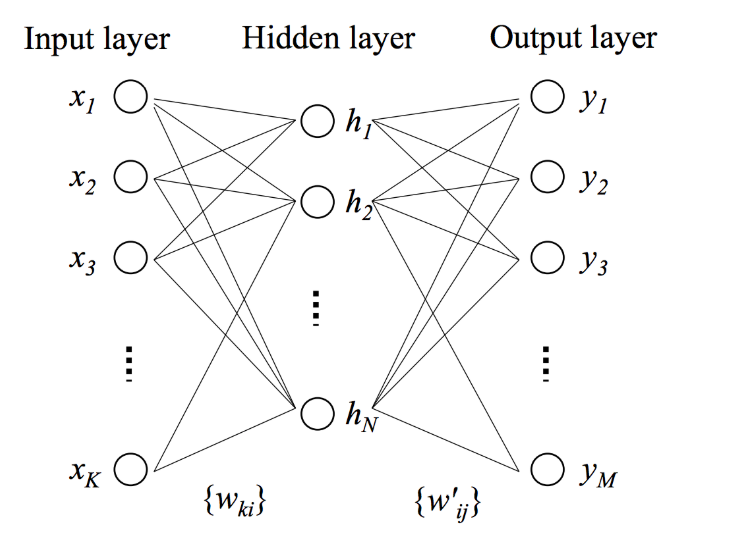
\includegraphics[width=0.5\textwidth]{images/nn.png}
\caption{A one layer NN network}
\label{Simple NN}
\end{figure}
We take a Neural Network (NN) as shown in fig \ref{Simple NN}} with the following parameters, 
\begin{itemize} 
\item Input vector of length of K, $x = (x_1, x_2, x_3, ....., x_K)$. 
\item Hidden layer consists of N neurons $h = (h_1, h_2, h_3, ....., h_N)$. 
\item Ouput layer is of size M, $\textbf{y} = (y_1, y_2, y_3,...., y_M)$. 
\end{itemize}
Every neuron in the input layer is connected to all the neurons in the hidden layer, the connection weight between neuron i and k is given by $w_{ki}$. Similarly, all the neurons in the hidden layer are connected to the output layer, the connection weight between the ith hidden neuron and j th output neuron is given by $w_{ij}'$.\\
We can think of $w_{ki}$ as the k,i entry in the matrix $\mathbf{W}^{K \times N}$, similarly $w_{ij}'$ can be considered as the i,j entry in the $\mathbf{W}^{K \times N}'$,. The activation function f is the sigmoid activation function.
\\ 
\\
\textbf{Forward Pass}
The forward pass can be expressed by the following equations, 
\begin{align}
&h_i = f(u_i) = f(\sum_{k=1}^K w_{ki} x_k) \hspace{0.8pt} [\text{This is the ouput of the i th neuron in the hidden layer }] \\
&y_j=f(u_{j}^{'})=f(\sum_{i=1}^K w_{ij}^{'} h_i) \hspace{0.8pt} [ \text{This is the ouput of the j th neuron in the ouput layer} ] \\
&\text{if we assume a Mean Squared Error Loss} \\
&E(x) = \frac{1}{2} \sum_{j=1}^M (y_j - t_j)^2
\end{align}
\newpage
\textbf{Backward Pass}\\
In the backward pass we compute the loss and gradient of loss wrt(with respect to) to all the parameters($\mathbf{W}$) in the NN. We the pass these gradient back and update the parameters of the network.
\begin{align}
&\frac{\partial E(x) }{w_{ij}^{'}} = \frac{\partial E(x)}{\partial{y_j}} \frac{\partial{y_j}}{\partial{u_{j}'}}\frac{\partial u_{j}'}{w_{ij}'}\\
&\frac{\partial E(x)}{\partial{y_j}} = \sum_{i=1}^M (y_{j} - t_{j}) \\
&\frac{\partial{y_j}}{\partial{u_{j}'}} = y_j (1-y_j) \\
&\frac{\partial u_{j}'}{w_{ij}'} = h_i
\end{align}
Hence, 
\begin{align}
&\frac{\partial E (x)}{w_{ij}^{'}} = \sum_{i=1}^M (y_j - t_j) y_j (1 - y_j) h_i
\end{align}
Similarly we can get, \begin{align}
\frac{\partial E(x)}{w_{ki}} = \frac{\partial E}{\partial y_j}\frac{\partial y_j}{\partial u_{j}'}\frac{\partial u_{j}'}{\partial h_i}\frac{\partial h_i}{\partial u_i}\frac{\partial u_i}{\partial w_{ki}}
\end{align}

This is the famous Backpropogation algorithm it is so called, because we are back propagating the gradients from output to the input.\\
The update rule for parameters  is given by 
\begin{align}
w_{ij}'^{+} = w'_{ij} - \eta * \frac{\partial E(x) }{w_{ij}'}
\end{align}
where $\eta$ denotes the learning rate. \\
\subsection{Gradient Descent }
Back propagation only computes the gradient for only one sample, in practice back propagation is generally combined with learning algorithms such as gradient descent which computes the gradient for all the samples in the training data. Hence, Gradient Descent update rule is given by 
\begin{align}
w_{ij}'^+ = w_{ij}' - \frac{\eta}{N} \sum_{x}  \frac{\partial E(x) }{w_{ij}'}
\end{align}
For ease of discussion we now employ the following convection for parameter updates 
\begin{align}
\theta_{t+1} = \theta_{t} - \frac{\eta}{N} \sum_{i=1}^N \nabla(f(x_i; \theta_t))
\end{align}
Here f denotes the Loss function and $x_i$ denotes the i th point in the dataset $\mathcal{D}$ of size N . We can see that computing the gradient  for all of the N data points is computationally expensive. In practice only a part of dataset is used for computing the gradient and  updating of the parameters in one iteration. \\
\subsection{Stochastic Gradient Descent (SGD)}
The stochastic gradient estimates the true gradient on the whole dataset by using only a single data point. The update rule for the SGD algorithm is given by 
\begin{align}
\theta_{t+1} = \theta_{t} - \eta \nabla(f(x_i; \theta_t)) \label{SGD}
\end{align}
We can show that the stochastic gradient  $\nabla(f(x_i; \theta_t)$ is an unbiased estimate of the true gradient $\nabla(f(; \theta_t)$, if we assume that the samples are iid (independent identically distributed) and we choose any point uniformly at random then, 
\begin{align}
E(\nabla(f(x_i; \theta_t))) = \frac{1}{N} \sum_{i=1}^N \nabla(f(x_i; \theta_t) 
\end{align}
This shows that the stochastic gradient estimate is unbiased, but the variance of stochastic gradient algorithm is non-zero as shown below , \\
Using Taylor Series and assuming that f is an L-smooth function we get
\begin{align}
\E f(x; \theta_{t+1}) &\leq \space  \E f(x; \theta_t) - \eta \E \big(\nabla f(x, \theta)^T (\theta_{t+1} - \theta_{t})\big) - \frac{L\eta^2}{2} \E || (\theta_{t+1} - \theta_{t}) || ^2 \\
& \leq \E f(x; \theta_t) - \eta ||\E \nabla  f(x; \theta_{t})||^2 - \frac{L\eta^2}{2} \E ||t\nabla f(x; \theta_{t})||^2  \hspace{1.2pt} \text{[Using Eq \ref{SGD}]} \\ 
&\leq \E f(x; \theta_t) - \eta ||\E \nabla f(; \theta_{t})||^2 - \frac{L\eta^2}{2} \E\Big[ \nabla f(x; \theta_{t})^2\Big] \\
&\leq \E f(x; \theta_t) - \eta(1 -\frac{L\eta}{2}) ||\E \nabla f(; \theta_{t})||^2 + \frac{L\eta^2}{2}  \mathbb{V}(\nabla f(x ;\theta)) \label{Variance Red}
\end{align}
Where , $\mathbb{V}(\nabla f(x; \theta)) = \E || \nabla f(x; \theta) - \E\nabla f(x; \theta)||^2 $.\\\\
From the above Eq \ref{Variance Red} it can be easily seen that a smaller variance helps in getting to a better optimal solution faster.\\ In the next chapter we see some popular techniques in literature that have been used for variance reduction.

\chapter{Variance Reduction Techniques}

Variance Reduction\footnote{The major Source of this chapter is Handbook of Monte Carlo Methods} is an important part of many approximation algorithms like SGD@. These techniques help in finding a more precise approximation quantity of intreset resulting in a better performance models that are being trained using these approximation algorithms. Variance reductions techniques have found usage in a variety of machine learning applications like MCMC algorithms, Policy Gradients and SGD all of which use variance reduction techniques for a better generalisation perfomance of the model being trained. 

This chapter discusses about the existing methods of variance reduction in literature. We study all the techniques from the point of view of Monte Carlo Estimation of $E(f(x))$ but all this also readily applies to Stochastic Gradient Algorithms. We give references to those papers that use these techniques for SGD and describe in detail in section\ref{related_work}. \\ \\
In this chapter we, firstly give a brief introduction to Monte Carlo Estimation and then introduce variance reduction techniques such as Stratified Sampling, Control Variates and Importance Sampling


\section{Basics}
To motivate our discussion for importance sampling we take the problem of finding the mean of a function of a Random Variable. 
Consider a random variable X having probability mass function or probability density function denoted by $p_X(x)$ which is greater than zero on a set of values $\mathcal{X}$. Then the expected value of a function f(X)is given by, 
\begin{equation}
\E (f(X)) = \sum_{x\in\mathcal{X}} f(x) p_{X}(x)
\end{equation}
if X is discrete and, 
\begin{equation}
\E (f(X)) = \int_{x\in\mathcal{X}} f(x) p_{X}(x) dx
\end{equation}
if X is continuous \\
If we were to take n samples of $(x_1, x_2, ........, x_n)$ and compute the mean of f(x), we get \footnote{\label{Basics} Here we assume the samples are iid.} of $\E (f(X))$\begin{equation}
	\widetilde{f}_{n} (X) = \frac{1}{n} \int_{x\in\mathcal{X}} f(x)dx
      \end{equation}

$\widetilde{f}(X)$ is called the monte carlo estimate of $\E (f(X))$ . If $\E (f(X))$ exist then Weak Law of Large Numbers tells us that for any arbitarily small $\epsilon$
\begin{equation}
	 \lim_{n\rightarrow \inf} P (|\widetilde{f}(X)  - \E (f(X))| \geq \epsilon)=0.
\end{equation}
This simply states that as n increases our approximation get closer to the exact value. \\
Every stochastic approximation algorithm contains two important concepts, bias and variance. 
\begin{itemize}
\item Bias can be defined as the mean of difference between the estimated and the exact value of a Random Variable. 
More formally for the above example, 
\begin{equation}
	Bias(\widetilde{f}(X)) = \E (\widetilde{f}(X) - \E (f(X)))
\end{equation}
An estimator is called unbiased if its bias is equal to zero.
\\
\item Variance can be defined as the measure of dispersion between estimates from the exact quantity. For the above example we have 
\begin{equation}
	Var (\widetilde{f}(X)) = \E [\{\widetilde{f}(X) - \E (f(X)\}^2]
\end{equation}
\end{itemize}
\newtheorem{lemma}[theorem]{Lemma}
If we assume the samples are IID. We can show that Monte Carlo Estimates are unbiased.

\begin{equation}
	\E (\tilde{f}(X)) = \E \left(\frac{1}{n} \int_{x\in \mathcal{X}} f(x) dx\right) = \frac{1}{n} \int_{x \in \mathcal{x}} \E (f(x)) dx= \E (f(X)) 
    \end{equation}
The variance of Monte Carlo Estimates is given by the following 
\begin{equation}
Var(\tilde{f}(X)) = Var\left(\frac{1}{n}\int_{x \in \mathcal{X}} f(x) dx\right) = \frac{Var(f(X))}{n} = \frac{1}{n} \int_{x\in\mathcal{X}} [f(x) - \E (f(X)]^2 p_{X}(x) dx
\end{equation}
the variance of the estimator is non zero this could lead to catastrophic results for the subsequent models that uses this quantity. To have a better approximation we need to reduce is the variance this is the goal of variance reduction methods. Below we list and explain some popular methods to achieve variance reduction.

\begin{itemize}
\item Stratified Sampling 
\item Control Variates 
\item Importance Sampling
\end{itemize}

\newpage
\section{Stratified Sampling}

Consider estimation of  $\theta = E[f(X)] =\int_{x\in\mathcal{X}} f(x) p(x) dx $. For stratified sampling, we first partition the domain of integration $\mathcal{X}$ into m disjoint subsets
$\mathcal{X}_i$ , i = 1, 2, . . . , m ie $ \mathcal{X}_i \cap \mathcal{X}_j = 0$ $ \forall i \neq j$ and $\cup_{i=1}^m \mathcal{X}_i= \mathcal{X}$. Defining 
\begin{align}
\E (\theta_i) &= \E (f(X) | X\in \mathcal{X}_i)\\
					&= \int_{\mathcal{X}_i} f(x) p(x) dx
\end{align}
for i=1,2 ..... m. We can write 
\begin{equation}
		\theta = \int_{\mathcal{X}} f(x) p(x) dx = \sum_{i=1}^m \int_{\mathcal{X}_i} f(x) p(x) dx = \sum_{i=1}^m \theta_i
\end{equation}


The motivation behind this method is to to sample more from regions that have more variability or diverseness, rather than sampling evenly across the whole region S. \\
We now derive the mean and variance for stratified sampling
Define 
	\begin{align}
	&g_i = \int_{\mathcal{X}_i} p(x) dx \\
    & \text{and} \\
    & p_i(x) = \frac{1}{g_i} p(x)
	\end{align}
    Then $\sum_{i=1}^m g_i =1$ and 
    \begin{equation}
    \int_{\mathcal{X}_i} p_i (x) dx = 1
    \end{equation}
By expressing 
\begin{equation}
f_i(x) = 
\begin{cases}
f(x), \space \text{if} \space x \in \mathcal{X}_i \\ 
				0, \text{otherwise}
\end{cases}
\end{equation}
we can see,
\begin{align}
	\theta_i = \int_{\mathcal{X}_i} g_i f(x) \frac{p(x)}{g_i} dx
\end{align}
Using Monte Carlo Estimate for $\E(f(x_i))$ we get 
\begin{equation}
			\tilde{\theta_i} = \frac{g_i \sum_{j=1}^{N_i} f_i(x_j)} {N_i}
\end{equation}
where $x_1, x_2, ...... x_{N_i}$ are random samples from the distribution with density $g_i(x)$ with the variance given by 
\begin{equation}
	Var(\tilde{\theta_i}) = \frac{g_{i}^2 \sigma_{i}^2} {N_i}
\end{equation}
where $\sigma_{i}^2 = \text(Var) (f(x) | X \in \mathcal{X}_i)$ . Thus for the full the estimator 
\begin{equation}
\tilde{\E(f(X))} = \sum_{i=1}^m \tilde{\E(f(x_i))} = \sum_{i=1}^m \frac{g_i} {N_i} \sum_{j=1}^{N_i} f_i(x_j)
\end{equation}
with the variance given by 
\begin{equation}
Var(\theta) = \sum_{i=1}^m \frac{g_{i}^2 \sigma_{i}^2} {N_i}
\end{equation}

Variance reduction can now be cast as the following optimization problem
\begin{align}
\text{argmin}_{N_i} &Var(\tilde{\E(f(X))}\\
&\text{st } \sum_{i=1}^m N_i = N
\end{align}
using the Lagrangian Dual we get 
\begin{equation}
\sum_{i=1}^m \frac{g_{i}^2 \sigma_{i}^2 } {N_i} + \lambda (N - \sum_{i=1}^m N_i)
\end{equation}
The optimum value comes out to be $N_i = \frac{g_i{\sigma_i}N }{\sum_{i=1}^m g_i{\sigma_i}}$

The method is simple to understand and implement but it is not always possible to dive the data into mutually exclusive strata moreover estimating a value for $\sigma_i$(Variance of strata i) is hard and computationally expensive. 

\section{Control Variate}

We again use the problem of estimating $\theta$. Control Variate method find another function h(x) which is similar to f(x) such that $\E(h(x)) = \int h(x) p(x) dx = \tau $ is known, this function $h(x)$ is called the control variate. The equation $\theta = E[f(X)]$ can equivalently be written as  
\begin{equation}
	\theta = \int [f(x) - h(x)] p(x) dx + \tau = \E[f(x) - h(x)] + \tau
\end{equation}
The Monte Carlo estimate for above equation is 
\begin{align}
&\widetilde{\theta} = \frac{1}{N} \sum_{i=1}^N [f(x_i) - h(x_i)] + \tau,  \\
& \text{and} \\
& var(\tilde{\theta}) = \frac{var(f_x) + var(h_x) - 2 cov(f(x), h(x))}{N}
\end{align}
The variance of the estimator can be reduced if we choose the above the $h(x)$ such that 
\begin{equation}
corr(f(x), h(x)) > \frac{1}{2}
\end{equation}
$corr$ denotes the correlation between $f(x)$ and $h(x)$ 

Finding such a $h(x)$ is not trivial and sometimes not possible for many problems. We now look at the most popular variance reduction technique in literature Importance Sampling. 

\section{Importance Sampling }
Importance sampling attempts to reduce the variance of the Monte Carlo estimate by changing the distribution from which the actual sampling is carried out.\\ Monte Carlo estimates uses samples generated from the underlying distribution of x (with density p(x)). Suppose that it is possible to find another distribution H(x) with density h(x) with the property that $\frac{f(x)p(x)}{h(x)}$ has a small variance. Then $\theta$ can be expressed as
\begin{equation}\label{Imporatnce Sampling}
\theta =\int f(x)g(x)dx =\int  f(x) \frac{p(x)} {h(x)} h(x)dx = \E_{h(x)} [\phi(x)]
\end{equation}

where $\phi(x) = \frac{f(x) p(x)} {h(x)}$ and the expectation is with respect to H . Now the monte carlo estimate for $\theta$ becomes 
\begin{equation}
\widetilde{\theta} = \frac{1}{N} \sum_{i=1}^N \phi(x_i) 
\end{equation}
where $x_i = x_1, ......, x_n$ is sampled from H. The variance of this estimator is given by 
\begin{equation}\label{Variance Importance Sampling}
var(\widetilde{\theta}) = \frac{1}{N} \int (\phi(x_i) - \theta)^2 h(x) dx = 
\frac{1}{N}\int  \Big(\frac{f(x)p(x)}{h(x)}\Big)^2  h(x) dx  -\frac{\theta^2}{N}
\end{equation}
For variance reduction we need, 
\begin{equation}
\int  \Big(\frac{f(x)p(x)}{h(x)}\Big)^2  h(x) dx  \leq \int f(x)^2 p(x) dx 
\end{equation}
Below we show that the optimal distribution for variance reduction is of the form $h(x) \propto f(x) p(x)$. \\
\begin{claim}
It can be easily shown that if $h(x) = \frac{f(x) p(x)} {c}$ then for any other distribution 
$\hat{h(x)}$. Var(h(x)) $\leq$ Var ($\hat{h(x)}$).
\end{claim}
\begin{align}
Var(\widetilde{\theta})_{h(x)} - \frac{\theta^2} {N} &= \int  \Big(\frac{f(x)p(x)}{h(x)}\Big)^2  h(x) dx \\
&= \bigg(\int \Big(f(x)p(x) dx \Big)   \bigg)^2 \label{36} \\ 
&= \bigg(\int \Big(\frac{f(x)p(x)}{q(x)}q(x) dx \Big)\bigg )^2 \\
&\leq \int \Big(\frac{f(x)^2p(x)^2}{q(x)^2}q(x) dx )\Big)  \label{c-s} \\ 
&\leq \int \Big(\frac{f(x)^2p(x)^2 dx}{q(x)} \Big) \\
&\leq Var(\widetilde{\theta})_{\hat{h(x)}} - \frac{\theta^2} {N}
\end{align}
\\
We get \ref{36} setting h(x) = $\frac{f(x)p(x)} {c}$ and using c = $\int (f(x)p(x) dx)$ \\
\ref{c-s} using Cauchy-Schwartz Inequality.

From the above discussion we have shown that the importance sampling methods are easiest to optimize for variance reduction and suffer from no faults like how to distributed the data into strata or how to define control variate.
These are the major reason we prefer to use importance sampling in our work instead of the other two methods described above.

\chapter{Submodularity and Diversity }

Submodular functions are a well know and widely studied class of functions defined on sets. Diversity is an very important topic in the context of Machine Learning. Finding a set of diverse items is a hard and important task and finds application in the filed of Document/ Video Summarization, Facility location problems etc. Submodular functions have a natural diminishing return property which makes them suitable for modeling diversity. Submodular function have used in wide variety of problems like Graph Cut, Facility location, Document Summarization etc. \\
In this chapter we first define submodular functions. Then discuss how submodular functions have been used in variance reductions tasks in existing literature. Optimization of submodular functions is discussed later for the case of large datasets. Finally, the relationship between submodular functions and diversity through is explained through an example.


\section{Submodularity}

Submodularity is a property of a set function that assigns a value to each of the the subsets of the set. ie  $ f: 2^V \rightarrow \mathbb{R}$. This can be thought of as assigning a utility value to each subset.
\theoremstyle{definition}
\begin{definition}{Submodular:}
For a set function $ f: 2^V \rightarrow \mathbb{R}$ is submodular if for every $ A \subseteq B \subseteq V $ and e $\in$ V $\setminus$ B it holds that 
\begin{equation}
			f(A \cup e) - f(A) \geq f(B \cup e) - f(B)
\end{equation}
\end{definition}
Equivalently , a function $ f: 2^V \rightarrow \mathbb{R}$  is submodular if for every A, B $\subseteq$ V, 
\begin{equation}
f(A\cap B) + f(A \cup B) \leq f(A) + f(B)
\end{equation}
The first definition can intuitively be explained as , the increase in uitility of subsets A and B after adding an element e(not present in B) is greater for the set with smaller size. This is called the diminishing return property of submodular functions.
\\

\theoremstyle{definition}
\begin{definition}{Monotonicity :}
A set function $f:2^V\rightarrow \mathbb{R}$ is monotone if for every $A \subseteq B \subseteq V,$ f(A) $\leq$ f(B)
\end{definition}
\newpage
\theoremstyle{definition}
\begin{definition}{Discrete Derivative}
For a set function $f:2^V\rightarrow \mathbb{R}$, $S \subseteq V$ and $e\in V$, let $\Delta_{f}(e|S):= f(S \cup \{e\}) - f(S)$ be the discrete derivative of f at S with respect to e.
\end{definition}
Discrete derivative is also commonly know as marginal gain of f on S with e. Next we go through some important examples of submodular functions used in practice.

\subsection{Examples}

\begin{itemize}
\item Facility Location: Suppose we want to select some locations out of a set V = {1, . . . , n}, to open up facilities in order to serve a collection of m customers. If we open up a facility at location j, then it provides service of value $M_{i,j}$ to customer i, where $ M \in R_{m\times n}$ . If each customer chooses the facility with highest value, the total value provided to all customers is modeled by the set function
\begin{equation}
f(S) = \sum_{i=1}^m max_{j\in S} M_{i, j}
\end{equation}

\begin{claim}
   $f(S)$ is a submodular function.
\end{claim}
\begin{proof}
        We need to show that $\triangle_{f}(e|A) \leq \triangle_{f}(e|b)$ where $A \subseteq B \subseteq V$ for the funtion $f(S)$ to be submodular. Consideer the following cases\\
        \text{Case I} If $\triangle_{f}(e|B) = 0 then \triangle{f}(e|A) =0$. Hence we have the $\triangle_{f}(e|B) = \traingle{f}(e|A)$\\
        \text{Case II} If $\triangle_{f}(e|A) \leq 0$ and $\triangle_f(e|B) = 0$ then we have $\triangle_f(e|A) \leq \triangle_{f}(e|B)$\\
        \text{Case III} If $\triangle_{f}(e}|B) \leq 0$ then $\triangle_{f} (e|A) = \triangle_{f}(e|B)$\\
        In all the above cases we have $\triangle_{f}(e|A) \leq \triangle_{f}(e|B)$. Hence $f(S)$ is a submodular function.
\end{proof}
\item Entropy: Given a joint Probability Distribution P(X) over a discrete-valued random vector $X = {X_1, X_2, ... X_n}$, the function f(S) = H($X_s$) is monotone submodular, where 
\begin{equation}
				H(X_s) = - \sum_{x_S} P(x_S) log_2 P(x_S)
\end{equation}
where we use the notational convention that $X_S$ is the random vector consisting of the coordinates of X indexed by S, and likewise $x_S$ is the vector consisting of the coordinates of an assignment x indexed by S. \\
\begin{claim}
To show that $H: 2^S \rightarrow [0, \inf)$ is submodular consider:
\end{claim}
\begin{proof}
\begin{equation}
H(X, s) - H(X) \geq H(Y, z)  -H(Y) = H(z|X) \geq H(z|Y)
\end{equation}
where $H(z|Y ) = H (z|X \cup (Y \setminus X)) \geq H(z|X)$, since conditioning cannot increase entropy.
\end{proof}
\end{itemize}


\subsection{Optimization of Submodular Functions}
The application of submodular functions in so many areas makes it naturally to study submodular optimization. In our work we are interested in the maximization of submodular functions. Formally,  
\begin{equation}
	\text{max}_{S\subseteq V} f(S) \hspace{1.8pt} \text{subject : to constraints on S}
\end{equation}
the most basic constraint is called the cardinality constraint which is $ |S| \leq$ k for some k. Even in a the simple example of trying to find the best k places to eat for maximum fun, this problem is NP-Hard. Though this problem can solved very efficiently using the Greedy algorithm from \cite{nemhauser} if $f(S)$ is submodular. 

\subsection{Greedy Algorithm}

\begin{algorithm}
\caption{(Greedy) Algorithm by \cite{nemhauser}}
\label{Greedy}
\begin{algorithmic}[1]
\Require{Set V, Set function $f : 2^V \rightarrow \mathbb{R}$, Size of subset k.}
\Ensure{Subset $S_k \subseteq V$ of size k}
\State $S_0= {\phi}$ 
\For{$i=0$ to $k$}
\State $ v_{*} \leftarrow argmax_{v\ in V\setminus S_{i−1}} \Delta (v|S_{i-1})$
\State $S_i \leftarrow S_{i-1} \cup {{v_*}}$
\EndFor
\end{algorithmic}

\end{algorithm}
\theoremstyle{definition}
\begin{theorem}
 Fix a nonnegative monotone submodular function
$f : 2^V \rightarrow \mathbb{R}^+$ and let ${S_{i:i\geq0}}$
be the greedily selected sets defined in \ref{Greedy}
Then for all positive integers  k and l, 
\begin{equation}
f(S_l) \leq (1 - e^{-l/k})\space max_{S:|S|\leq k} f(s)
\end{equation}
In particular, for l=k, $f(S_k) \geq (1- 1/e) \space max_{|S|\leq k} f(S)$
\end{theorem}
\begin{proof}
 Let $S^* \in \text{argmax} \{f(S) : |S| \leq k\}$  be an optimal set of size k (due to monotonicity of f we can assume w.l.o.g. it is of size exactly k), and order the elements of $S^∗$ arbitrarily as ${v^{*}_{1}, . . . , v^{∗}_k}$. Then we have the following sequence of inequalities for all i < l,
 \begin{align}
 f(S^*) &\leq f(S^* \cup S_i) \label{eq1}\\
 		&= f(S_i) + \sum_{i=1}^k \Delta(v_j^* | S_i \cup \{{v^{*}_{1}, . . . , v^{∗}_k}\}) \label{eq2} \\
        &\leq f(S_i) + \sum_{v\in S^*} \Delta(v | S_i) \label{eq3}\\
        &\leq f(S_i) + \sum_{v\in S^*}  (f(S_{i+1} - f(S_i)) \label{eq4}\\
        &\leq f(S_i) + k(f(S_{i+1} - f(S_i)) \label{eq5}
 \end{align}


The first equation \ref{eq1} follows from Monotonicity of f. The next inequality \ref{eq2} is from the telescoping sum. \ref{eq3} uses Sub modularity . \ref{eq4}  holds because $S_{i+1}$ is built greedily from $S_i$ in order to maximize the marginal benefit $\Delta(v | S_i)$, and \ref{eq5} merely reflects the fact that $|S^∗| \leq k$. Now define $\delta_i := f(S^*) - f(S_i)$ we get 
\begin{equation}
	\delta_{i+1} \leq (1 - \frac{1}{k}) \delta_i
\end{equation}
Hence, $\delta_l \leq (1 - \frac{1}{k}) ^ l \delta_0$. Next, $\delta_0 = f(S^*) - f(\phi) \leq f(S^*)$ since f is nonnegative by assumption, using $1-x \leq e^{-x}$  for all $x \in \mathbb{R}$ we have 
\begin{equation}
\delta_l \leq \Big(1 - \frac{1}{k}\Big)^l \delta_0 \leq e^{-l/k} f(S^*) 
\end{equation}
Rearranging we get $f(S_l) \geq (1 - e^{-l/k})f(S^*)$
\end{proof}

Though the Greedy Algorithm\ref{Greedy} is pretty simple to implement it suffers from a major flaw that it does not scale well for large datasets. In particular the run time for the Greedy Algorithm is $0(n*k)$ function evaluations which is prohibitively expensive even for moderate size n(number of data points).\\
To decrease the number of function evaluation the LAZY-GREEDY algorithm by \cite{minoux1978accelerated} is proposed. The LAZY-GREEDY algorithm cleverly makes use of submodularity to reduce the running time by keeping the elements in a sorted decreasing order based upon the marginal gains, at each iteration i, it evaluates the element on top of the list, say e, and updates its upper bound, $\rho(e) \leftarrow \Delta(e|S_{i -1})$. If after the update $\rho$(e) $\geq$ $\rho$(e') for all e' $\neq$ e, submodularity guarantees that e is the element with the largest marginal gain. The worst case bounds for LAZY-GREEDY algorithm are similar to the Greedy algorithm but in practice it boost the the speed up by order of magnitudes. Still for a large k(cardinality constrain) and repeated selection of points the LAZY-GREEDY algorithm is still slow and impractical to be applied.

\subsection{STOCHASTIC-GREEDY} \label{lazier}

STOCHASTIC-GREEDY \cite{mirzasoleiman2015lazier} algorithm tries to improve upon the LAZY-GREEDY algorithm using a very simple insight of sub sampling the dataset before using the LAZY GREEDY or GREEDY algorithm. It is in a sense equivalent to stochastic gradient descent which improves the running time of gradient descent for convex optimization using a sub sampling step.
\
\begin{algorithm}
\caption{STOCHASTIC GREEDY Algorithm by \cite{mirzasoleiman2015lazier}}
\label{SGreedy}
\begin{algorithmic}[1]
\Require{set V, set function $f : 2^V \rightarrow \mathbb{R}$, Size of subset k.}
\Ensure{subset $S_k \subseteq V$ of size k}
\State $S_0= {\phi}$ 
\For{$i=0$ to $k$}
\State R $\leftarrow$ a random subset of size $\frac{n}{k\log(\frac{1}{\epsilon})}$, obtained by sampling from $V \setminus S_{i-1}$.
\State $ v_{*} \leftarrow \text{argmax}\space \space \Delta_{v\in R}(v| S_{i-1})$
\State $S_i \leftarrow S_{i-1} \cup {{v_*}}$
\EndFor
\end{algorithmic}
\end{algorithm}

STOCHASTIC-GREEDY algorithm is the  first linear-time algorithm for maximizing a non-negative monotone submodular function subject to a cardinality constraint k. STOCHASTIC-GREEDY achieves a (1 - 1/e - $\epsilon$) approximation guarantee to the optimum solution with running time O(n log(1/$\epsilon$)). Achieving a approximation ratio of (1 - 1/e -$ \epsilon$) requires $R \geq n/k log(1/\epsilon)$ for further details the readers is implored to read \cite{mirzasoleiman2015lazier}\\
There have been other recent works \cite{tschiatschek2018differentiable} that show that rather than taking the max element we could also select the elements according to the probability conditioned on the marginal gain of the elements. 


\section{Variance Reduction and Submodularity }

Variance reduction and Submodularity look pretty unrelateded at start but as shown below for certain problems we can cast the variance reduction problem as a submodular maximization problem.
\\
Let us consider the case where we have a finite number of locations V and we can place a sensor at each location to observe a associated quantity with these locations given by $X_v$, the joint probability of the observations is given by $P(X_v)$. We want to reduce the cost of placing the sensors choosing only a subset of locations A $\subseteq$ V to observe, the locations A have to selected such that the average predictive variance, 
\begin{equation}
	V(A) = \frac{1}{n} \sum_{i} \sigma_{i|A}^2
\end{equation}
is minimized. $\sigma_{i|A}^2$ denotes the predictive variance at the location i. 
\begin{equation}
\sigma_{i|A}^2 = \int P(x_A) \E\Bigg[ (X_i -\E[ X_i | x_A])^2 | x_A\Bigg] dx_A
\end{equation}
We need to solve the following optimization problem for getting the minimum average predictive variance.
\begin{equation}\label{optimsation}
A^* = argmin_{|A| \leq k} V(A)
\end{equation}
As can be seen clearly that \ref{optimsation} problem has a combinatorial search space which makes the problem hard to solve. It can be show that the problem is NP-hard in general \cite{das2008algorithms}. Fortunately \cite{das2008algorithms} show that the variance reduction 
\begin{equation}
F_s(A) = \sigma_s^2 - \sigma_s|A ^2
\end{equation}
at any particular location s, satisfies the following diminishing returns behavior: Adding a new observation reduces the variance at s more, if we have made few observations so far, and less, if we have already made many observations. Since now we can say that each of $F_S(A)$ is submodular, the average variance reduction is also submodular 
\begin{equation}
	F(A) = V(\phi) - V(A) = \frac{1}{n} \sum_{s} F_s(A)
\end{equation}
It can also be shown that the average variance reduction is monotonic ie for all A $\subseteq$ B $\subseteq$ V it
holds that F(A) $\leq$ F(B), and normalized F($\phi$) = 0. \\
Hence the problem of minimizing the average variance is an instance of the problem 
\begin{equation}
max_{A\subset V}F(A) , \text{subject to} |A| \leq K, 
\end{equation}
since F is monotonic, normalized, submodular we can use the above mentioned optimization methods to solve the problem easily. \\
A particular case of the above example is seen in the case of GeoStatistics in Kriging variance reduction minimisation problem and also in the Gaussian Process predictive variance reduction problem. \\

\section{Diversity and Submodularity}

Diversity of a set can be defined as the measure of difference between the elements of the dataset.  Diversity is a very important concept in area of Machine learning particularly in area of Result Diversification. A recommender's output should be diverse enough to capture the preferences of the user but not too diverse so that user preferences are orthogonal to the recommended items. Diversity is also an important requirement in the task of summarization of videos and text data. \\
The problem of adding a subset V (of size of k) to a already sampled set $S^*$ (of size m), such that we get the maximum diversity can be cast as the following optimization problem

\begin{equation}\label{diversitynphard}
\text{argmax}_{V \in S\setminus S*, |V|\leq k}\space f(V\cup S^*) - f(S^*)
\end{equation}
Where $f$ is a set function from $f:2^S \rightarrow \mathbb{R}$ that denotes the value of diversity of the set. It can be shown that problem is NP-hard in general and candidate solution space is very large. But if $f$ is submodular the problem can be solved as a Submodular Optimization problem which as seen earlier is a much easier problem to solve. From this we see that Submodular function are good candidates for modeling diversity in any problem this can be attributed to their diminishing return property.\\

We now show a example\cite{tschiatschek2016learning} of how a submodular function can model diversity. 
Let $f$ be a set function, $f : 2^S \rightarrow \mathbb{R}$ of the following form 
\begin{equation}\label{Diversity2}
	f(S) = \sum_{i\in S} u_i + \sum_{d=1}^L (\text{max}_{i\in S} \space w_{i, d} - \sum_{i \in S} w_{i, d} )
\end{equation}

Here $u_i$ indicates a modular functions which denotes the quality of the element i.
this term only captures frequencies of the individual items, ignoring any inter dependencies between the items. For countering this, the paper assigns to each item i an L-dimensional vector $w_i \in R^L_{ \geq 0} $. The intuition behind this is that each of these L dimensions will capture
some concept and can be interpret $w_{i,d}$ as a quantification of how relevant that
item i is for that specific concept d. To quantify the diversity of some items S $\subseteq$ V with respect to dimension d, the paper propose the term $\text{max}\space w_{i, d} - \sum_{i \in S} w_{i, d}$ . This
term is a non positive penalty, evaluating to 0 iff S contains at most one item i with positive value $w_{i,d} \geq 0$. Up until now we have shown a function that can model diversity, we now proved that the obtained function is submodular.  \\

\theoremstyle{claim} 
\begin{claim}
f(s) is a submodular function
\end{claim}
\begin{proof}
We take $A\subseteq B \subseteq S$, take an element v $\in S\setminus B$, then we assume 
\begin{align}
			& \Delta_f(v | A) \geq \Delta_f(v|B) \\
            & f(v \cup A) -f(A) \geq f(v \cup B) - f(B) \\
            & \text{Expanding and Simplying we get} \\
            &  \sum_{d=1}^L \big[(\text{max}_{i \in A \cup v} \space w_{i, d}) - (\text{max}_{i \in A} \space w_{i, d}) \geq  \sum_{d=1}^L \big[(\text{max}_{i \in B \cup v} \space w_{i, d} - \text{max}_{i \in B} \space w_{i, d})
\end{align}
We now show that this is always true when  A $\subseteq$ B since, 
\begin{itemize}
\item  Case 1: Assume that for some d $w_{v, d} \leq w_{i\in A, d}$ then LHS=RHS.
\item Case2: Assume that for some d $w_{v, d} \ge w_{i\in A, d}$ and $w_{v, d} \leq w_{i\in B, d}$. Using the fact that $w_{i, d} \geq 0 \forall{i}.\\ \text{LHS $\geq$ RHS}$
\item Case3:  Assume that for some d $w_{v, d} \geq w_{i\in B, d}$. Using the fact that $A \subseteq B$ means 
$w_{v, d} \geq w_{i\in A, d}$ But for any d $w_{i\in A, d} \leq w_{i \in B, d}$ . We see that $\text{LHS} \geq \text{RHS}$
Hence the above function is indeed submodular.
\end{itemize}
\end{proof}

\subsection{Probabilistic Submodular Functions}
\begin{definition}Probabilistic Submodular Functions: 
are probability distribution over $A \subseteq V$  of the form P(A) = $\frac{\pm exp(F(A)}{\mathcal{Z}}$. Where F(A) is a submodular function on V.
\end{definition}

  The normalizing quantity $\mathcal{Z} = P_{S\subseteq V} (exp \pm  F(S))$ is called the partition function, and − $\log \mathcal{Z}$ is also known as free energy in the statistical physics literature. 
A probabilistic way of modeling diversity is through use of Ising Models and Detrimental Point Processes as show in \ref{dpp_eq}\\
We can show that both Ising models and DPP are a special case of Probabilistic Submodular functions. 
In particular DPP is a distribution over set A of the form
P(A) = $\frac{exp(F(A))}{\mathcal{Z}}$ , where F(A) = $\log |L_Y|$. Here, L $\in \mathbb{R}
^{N \times N}$ is a positive semi-definite matrix, $L_Y^{'}$ is the square submatrix indexed by $Y^{'}$ and $|   |$ denotes the determinant. Because $L_y^{'}$ is positive semi-definite, F(A) is submodular, and hence DPPs are log-submodular. A major problem is the the complexity of sampling and learning these PSF for the case of large datasets.\\

From the above we have shown how existing methods make use of submodular functions to model diversity and how some existing methods can be categorized as special cases of submodular functions. We also show that diversity is and important metric to consider in many problems and that submodular functions model diversity well. A major problem with using submodular functions is the computation cost, in our work we come up with a novel submodular function which takes minimum amount to compute and also introduce methods to scale submodular optimization to large datasets.

\part{Related Work}\label{related work}
\chapter{Optimization Based Methods}
\section{Optimization Based Methods}
In this chapter we give a brief survey of the works that use optimization techniques to solve the variance reduction problem in SGD.\\

As stated earlier one of the major disadvantages of using mini batch SGD is random sampling of data points can lead to a large variance between the true gradient and the mini-batch gradient leading to slower convergence of SGD. Many techniques have been introduced to tackle this issue. 
\\
Variance Reduction techniques can broadly be classified into two categories namely non-sampling based and sampling based methods. Remember in mini-batch SGD we have 
\begin{equation}
\theta_{t+1} = \theta_t - \eta \frac{1}{B}\sum_{i=1}^B \nabla g(x_i; \theta_t )
\end{equation}
Where B denotes the size of the minibatch. If we choose B=1, the variance of the gradient can be shown to be 
\begin{align}\label{var-red}
\begin{split}
	Var(\nabla f(x_i; \theta_t)) &= \mathbb{E}[(\nabla f(x_i; \theta_t) -\nabla f( ; \theta_t)^2]\\
    &\nabla f(; \theta_t): \text{Full batch Gradient} \\
    &\nabla f(x_i; \theta_t): \text{mini batch Gradient}
\end{split}
\end{align}
For reduction in variance we can either change how we create mini-batches(importance sampling), change learning rate($\eta$), change batch size($b$) or change the way we updates the parameters. In this chapter we elaborate the non-sampling based/ optimization based techniques. 

\section{Non-Sampling Based}
These techniques sample the data points using a uniform distribution. These methods can further be specialized into the following categories \\
\textbf{Averaging Techniques}: These techniques reduce variance using averaging of parameter \cite{polyak1992acceleration} or by averaging of the gradients \cite{nesterov2013introductory}. Averaging based methods get smooth approximation of gradients or parameters, leading to a reduction in variance. 
\\
The simplest example of this method is the minibatch gradient decent algorithm, it can be shown that it reduces variance as follows,
Using Eq~\ref{SGD}
\begin{equation}
\theta_{t+1} = \theta_{t} - \eta \nabla(f(x_i; \theta_t)) 
\end{equation}
minibatch SGD changes the update rule to compute the gradient over a minibatch of data points $B = \{x_j \in \mathcal{D}\space|\spacej={1, 2, \ldots, b}\}$ as follows 
\begin{equation} \label{MSGD}
\theta_{t+1} = \theta_{t} - \frac{\eta}{b} \sum_{i=1}^B \nabla(f(x_i; \theta_t))  
\end{equation}

Where b denotes the size of a uniformly random sampled batch from full dataset $\mathcal{D}$. \\
Now using Eq~\ref{Variance Red} for minibatch SGD we get , 

\begin{equation}
\E f(x; \theta_{t+1}) \leq  f(x; \theta_t) - \eta(1 -\frac{L\eta}{2}) ||\E \nabla f(; \theta_{t})||^2 + \frac{L\eta^2}{2 b}  \mathbb{V}(f(x ;\theta) 
\end{equation}

Here we see that the variance reduces by factor b. Although, the computation cost has increase by a similar factor of b, this cost can be reduced using a parallel version of SGD but in general this cost is innocuous. In general minibatch gradient descent leads to a better generalization error in lesser time.
\\
\\
\textbf{Momentum} based techniques use momentum from past gradients to choose the descent direction\cite{johnson2013accelerating} \cite{schmidt2013minimizing}. The descent direction is based on the averaged descent direction, which is updated periodically. 
The simplest momentum based technique uses the following update rule 
\begin{equation}
\theta_{t+1} = \gamma \theta_{t} - \eta \nabla(f(x); \theta_t)) 
\end{equation}
where $\gamma \leq 1$ parameter. Momentum based methods reduce the oscillation in update of the parameters. It does so by adding a damping factor $\gamma$, the factor is useful when the direction of the gradient changes drastically the $\gamma$ factor dampens the update thereby reducing the update in the wrong direction. The gamma factor favours a smooth change of direction in gradients. As a result, we gain faster convergence and reduced oscillation. When momentum method is combined with minibatch SGD Eq~\ref{Variance Red} changes to 

\begin{equation}
\E f(\textbf{x}; \theta_{t+1}) \leq  f(\textbf{x}; \theta_t) - \eta(1 -\frac{L\eta}{2}) ||\E \nabla f(; \theta_{t})||^2 + \frac{\gamma^2 \eta^2}{2 b}  \mathbb{V}(f(\textbf{x} ;\theta) 
\end{equation}
Here we can see that addding the momentum term has reduced the variance further by a factor of $\gamma^2$.
\\
\\
\textbf{Adaptive Learning Rates and Batch Size}: Setting adaptive learning rates based on local curvature\cite{schaul2013no} or based on gradient information \cite{zeiler2012adadelta} has been proved to reduce variance in SGD. We show a particular case of AdaGrad Method, the update rule changes to 
\begin{equation}
	\theta_{t+1} = \gamma \theta_{t} - \frac{\eta} {\epsilon + G_t} \nabla(f(\textbf{x}; \theta_t)) 
\end{equation}
where $G_{t}^{D\times D}$,  is a diagonal matrix, where each diagonal element i, is the sum of the squares of the gradients w.r.t. $\theta^i_t$ (i th dimension of $\theta$) up to time step t , while $\epsilon$ is a small value added to avoid division by zero. Adagrad adapts the learning rate based on the parameters, performing smaller updates 
(i.e.\ low learning rates) for parameters associated with frequently occurring features, and larger updates (i.e.\ high learning rates) for parameters associated with infrequent features. For this reason, it is well-suited for dealing with sparse data. The interested reader is pointed to \cite{schaul2013no} for a more theoretical justification of variance reduction.
\\
Other papers have explored optimizing the batching size for variance reduction. These methods try to find a adaptive schedule for batch size that would reduce the variance. \cite{balles2016coupling} adapt batch size based on the variance of the gradient estimates, \cite{devarakonda2017adabatch} adaptively increases the batch size during the training process starting with a small batch size and doubling the batch sizes at specified intervals.\\

\chapter{Importance Sampling Based Methods}
Importance sampling based methods reduce the variance by finding an optimal distribution to sample the data points. As discussed earlier in case of importance sampling\ref{Imporatnce Sampling} instead to sampling from the distribution p(x) we try to find another surrogate distribution h(x) to sample the data points from. The tricky part is finding a distribution h(x) which is easy to sample from as well as it reduces the variance of the approximated function. Importance sampling methods have widely used in literature, below we discuss some of these which are our most relevant to our work.
\\
\section{Online Learning To  Sample \cite{bouchard2015accelerating}}
This is one of the first works to successfully show the usage of importance sampling methods for the case of Deep Learning models. The main ideas of the paper can be described as follows,   
The variance of importance sampling is given by Eq \ref{Variance Importance Sampling} 
\begin{equation}
var(\widetilde{\theta}) =  \frac{1}{N}\int  \Big(\frac{f(x)p(x)}{h(x)}\Big)^2  h(x) dx  -\frac{\theta^2}{N}
\end{equation}
Suppose that distribution comes from a family of distributions H(x; $\tau$), we can then optimize for the value of $\tau$ to find the best distribution that leads to maximum reductions in variance ,
\begin{equation}
var_{\tau}(\widetilde{\theta}) = \frac{1}{N}\int  \Big(\frac{f(x)p(x)}{h(x;\tau)}\Big)^2  h(x; \tau) dx  -\frac{\theta^2}{N}
\end{equation}
if $f(x) \in H(x; \tau)$ then, there exist a $\tau^*$ such that $h(x; \tau^*) \propto f(x)$. In general this is not true and also finding a closed form solution for the min $var_\tau(\tilde\theta)$ is not possible. The paper proposes for the use of an approximate learning method to solve the above problem as follows.  Taking the gradient wrt $\tau$  we get, 
\begin{align}
\nabla var_\tau(\tilde\theta) &= E_{h(x; \tau)}\Big(\frac{f(x)p(x)}{h(x;\tau)}\Big)^2 \\
& = E_{h(x; \tau)}\Big(\frac{f(x)^2 \nabla_{\tau} h(x;\tau)}{h(x; \tau)^3}\Big)\\
&= E_{h(x; \tau)}\bigg(\Big(\frac{f(x)}{h(x;\tau)}\Big)^2 \nabla_\tau\log h(x; \tau) \bigg)\\
\end{align}
 Now using SGD we can update a value for $\tau$ as, 
 \begin{equation}
 \tau_{t+1} = \tau_{t} - \eta \bigg(\Big(\frac{f(x_t)}{h(x_t;\tau)}\Big)^2 \nabla_\tau\log h(x_t; \tau) \bigg)
\end{equation}
here $x_t \sim h(x_t; \tau)$.

The paper is very innovative using SGD for solving the variance reduction problem in SGD. The paper is able to show decent results on many deep learning tasks like Image in painting , matrix factorization etc. \\ The paper suffers from a major drawback of solving another optimisation problem which requires both time and itself suffers from high variance, making the usability of the method limited. 
\section{Importance Sampling using Extra Information}

Another important recent work which has gained popularity is Adaptive Sampling for SGD by Exploiting Side Information\cite{gopal2016adaptive}. This work finds the distribution q(x) using additional information from the problem which it calls as side information. This side information can be anything like labels etc, is used to create bins and assign each data point to a its respective bin based on upon the side information of the data points. The paper proposes the following update rule 
\begin{equation}
\theta_{t+1} = \theta_{t} - \frac{1}{N} \frac{1}{P(i)}\nabla f(i; \theta_{t}) \\ 
\end{equation}
Where  $P(i) = \frac{p_k}{C_k}$ , this sampling scheme can be thought of as a two step process of the uniform sampling scheme, first sample any bin uniformly  $C_k$ at random and then sample from the bin according to the distribution $p_k$ which is the probability of selecting a data point inside bin k. If $p_k$ is equal to $C_k$ the above reduces to uniform sampling. Instead of keeping $p_k$ static the paper proposes a way of finding the optimal distibribution. The optimal distribution $p_k$ is found using the solution of the variance reduction problem for SGD@. The optimal distribution $p_k$ is expressed as follows, 
\begin{equation} \label{gopal}
p_k \propto \frac{|C_k|}{N} \sqrt[]{\frac{1}{|C|_k} \sum_{i \in C_k } || \nabla f(i; \theta_t} || ^2
\end{equation}
Intuitively, we select data points from bins that have a larger gradient. \\
This is a simple idea achieves great results on tasks of Logistic Regression but the method does not scale well to the larger datasets because of the need for calculating the gradient for finding $p_k$. Also it is not always possible to define side information for each and every dataset and problem.  

\section{Diversity based sampling}

Up until now we have only seen examples of sampling methods that consider the importance of samples individually. As stated earlier it is also important to consider the interactions of the samples in the minibatches with each other. The minibatches so constructed should be representative of the full dataset. In this section we elaborate how existing methods have tried to model this representativeness for usage in sampling methods for variance reduction.

\subsection{Mini-Batch Diversification}
One way of modeling representativeness and interaction of the samples is using diversity of the minibatch. In \cite{zhangdiversified} argue that creation minibatches that are diverse enough to be representative of the full dataset result in a variance reduction. Diversity of minibatch can be defined as the dissimilarity between data points of the minibatch in some metric space. Diversity serves a important purpose when sampling from the highly imbalanced datasets since it samples from less represented classes. \\
\begin{figure}[!htb] 
\centering
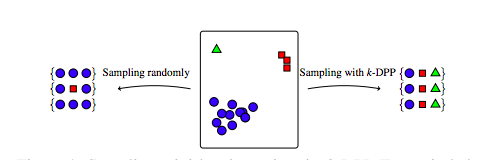
\includegraphics[width=0.5\textwidth] {images/diversity}
\caption{Example of DPP sampling on Imbalanced Dataset}
\label{Dpp_fig}
\end{figure}

As stated earlier Eq \ref{diversitynphard} diversity maximization is a NP-Hard Problem. The authors suggest using  Determinantal Point Process(DPP) for solving the diversity maximization problem. \\ DPP sampling firstly creates a similarity kernel matrix $\mathbf{L}$ , where $\mathbf{L}_{ij}$ denotes the similarity between data points i and j. The probability of sub sampling any subset Y of the set \{1,...,N\}, is proportional to the determinant of the sub-matrix $\mathbf{L_Y}$, 
\begin{equation} 
P(Y) = \frac{\text{det}(\mathbf{L}_Y )} { \text{det}(\mathbf{L}+I)} \propto \text{det}(\mathbf{L}_Y)
\end{equation}
a DPP based sampling approch promotes diversity as explained in section\ref{diversity_explaine}. The paper used a different variant of DPP sampling called the k-DPP sampling which is DPP sampling conditioned on given size k .
\begin{equation}
P_{L} ^ K (Y) = \frac{\text{det}(\mathbf{L}_Y )} { \sum_{|Y'| =k }\text{det}(\mathbf{L}_{Y}')} 
\end{equation}
 DPP sampling can be considered particular case of Probabilistic Submodular Function(PSF). Potentially other PSF can also be used to create diverse minibatches eg Repulsive Point Processes(RPP) eg \cite{zhang2018active}. A major issue with PSF based sampling methods is the computational time taken for sampling is approximated O($N^3$) ie cubic in the number of data points, though faster sampling methods have been proposed they are still pretty slow, this makes these methods infeasible for use in deep learning applications. 

\subsection{Active Bias Sampling}

In active bias sampling techniques we bias our probability distribution based on a particular criteria. The criteria can be anything from magnitude of loss \cite{katharopoulos2017biased}, gradient \cite{katharopoulos2018not}, lipschitz constant \cite{zhao2015stochastic} and variance of the samples \cite{chang2017active}. 

\subsection{Variance Reduction in SGD using Importance Sampling}
Until now we have not formally shown how a importance sampling methods can reduce variance. We now give a proof sketch to show importance sampling methods help in reducing variance SGD. We can rewrite the SGD update rule  defined in Eq \ref{SGD} for importance sampling as follows ,
\begin{equation}
\theta_{t+1} = \theta_{t} - \eta w_{I_t} f(x_{I_t}; \theta_t)
\end{equation}
Where $x_{I_t}$ is sampled from a probability distribution $P$ at time step t  ie $P(I_t = i) = p_i^t $, $w_{I_t}$ denotes the reweighing of the sample $x_{I_{t}}$, if $P = \frac{1}{N}$ and $w_{I_{t}} = 1$ the equation reduces to the standard SGD formulation.
\\
If we define the convergence speed S of SGD as the reduction of distance between the parameter $\theta$ and the optimal parameters $\theta^*$ in two consecutive iteration t and t+1.
\begin{equation}\label{chapter 8 eq1}
S = - \mathbb{E}_{p}[ || \theta_{t+1} - \theta^* || ^2 - || \theta_{t} - \theta^* || ^2 ]
\end{equation}
Also if we take $w_{I_t} = \frac{1}{N p_{I_t}}$ , taking the expectation of the gradient we get, 
\begin{equation}
E( w_{I_t} \nabla f(x_{I_t}; \theta_t)) = \frac{1}{N} \sum_{i=1}^N \nabla_{\theta_t}  f(x_{i_t}; \theta_t)
\end{equation}
Define $G_{I_t} = w_{I+t} \nabla f(x_{I_t}; \theta_t)$ using Eq \ref{chapter 8 eq1}
\begin{align}
S &= - \mathbb{E}_{P}[ || \theta_{t+1} - \theta^* || ^2 - || \theta_{t} - \theta^* || ^2 ] \\
&= - \mathbb{E}_{P} [\theta_{t+1}^T \theta_{t+1} - 2 \theta_{t+1} \theta^* - \theta_{t}^T\theta_{t} + 2 \theta_{t}^T \theta^* \\
& \text{Using the update rule and } G_{I_t}, \\
&= -\mathbb{E}_{P} [-2\eta(\theta_{t} - \theta^*) G_{I_t} + \eta^2 G_{I_t}^T G_{I_t} \\
&=2 \eta \theta_{t} - \theta^* \mathbb{E}_{P} G_{I_t} - \eta^2 E(G_{I_t})^T E(G_{I_t}) - \eta^2 Tr(V_{p_t}[G_{I_t}])
\end{align}

The proof is taken from \cite{katharopoulos2018not}. We can see that we can increase the convergence speed / reduce the variance of SGD if we find a optimal distribution that  minimizes $ Tr(V_{p_t}[G_{I_t}])$.
\cite{zhao2015stochastic} in their seminal work show that the optimal distribution for the above solution is  
\begin{equation}
p_t = \frac{G_{I_t}} {\sum_{I=1}^N G_{I_t}}
\end{equation}
It can be seen that the above distribution is computation very inefficient as it requires full gradient over the dataset for each time step t. A work around is approximate the $G_{I_t}$ by another quantity which is easier to compute as follows, 
\begin{align}
\text{min} &Tr(V_{p_t}[G_{I_t}]) \iff \text{min} Tr(V_{p_t} [H_{I}])\\
& H_I \geq G_{I_t}  \forall t
\end{align}
Then the optimal distribution is given by 
\begin{equation}
p_t = \frac{H_{I}} {\sum_{I=1}^N H_{I}}
\end{equation}
One proposed H is to use the Lipschitz constant of the Loss Functions f, since $G_{I_t} \leq L_I \forall {t}$.
In practice even using loss based sampling \cite{loshchilov2015online} and \cite{katharopoulos2017biased} performs really well. They test their implementation on many deep learning task for image classification and show good results. \\
All sampling based methods suffer from a slow speeds as they require the calculation of the probability distribution to sample the data points from. Also always choosing the data points using the most optimal distribution can lead to a decrease in performance in practice \cite{katharopoulos2018not}. This tradeoff between variance reduction and finding a probability distribution can be overcome if we use epsilon greedy strategy. Choosing data points using a random distribution in $\epsilon$ number of epochs and using importance sampling to select data points in $1-\epsilon$ number of epochs. The suggest using the following update rule for epsilon.

\\\begin{equation}\label{Fixed Eps}
\epsilon  = \epsilon * a + (1-a) * \left(1 - \frac{1}{\sum_{i=1}^N g_{i}^2} \left | \left | g - \frac{1}{|U|} \right| \right|^2 \right)^\frac{-1}{2}
\end{equation}
where $a  < 1 $ denotes the annealing term, g denotes the score vector for each data point assigned by the importance sampling distribution and U denotes the uniform sampling probability for the data point. They show that this really improves the performance of importance sampling schemes on large datasets that prevalent in Deep Learning. We also use this strategy in our experiments.


\part{Methodology}
\chapter{ Submodular Importance Sampling}
We now present our methodology for submodular importance sampling of mini-batches. Firstly a close relationship between diversity and submodularity is established, we then present our methodology for submodular importance sampling, a novel submodular scoring function is introduced that scales well for the needs of modern deep learning systems, and finally it is shown how our submodular importance sampling scheme leads to variance reduction in SGD.

As mentioned earlier, SGD samples data points randomly which can lead to mini-batches which are biased and present an inexact representation of the dataset. This consequently, leads to slow convergence. Diversity-based sampling methods attempt to sample data points such that the resulting mini-batch is a better representative of the full dataset. A simple example of diversity-based sampling is Stratified Sampling (\cite{zhao2014accelerating}) where data points are selected from strata, proportional to size/population of the strata, thereby leading to much more balanced minibatches. Submodular functions have been used earlier to model diversity in subset selection problem (\cite{tschiatschek2016learning}), recommendation systems \cite{ashkan2015optimal} etc. We exploit this submodular nature of diversity measures for the creation of diversified minibatches. 

%We show that our method, \myalgo, reduces variance in SGD based algorithms by creation of diversified mini batches.Section 3.1 discusses about submodular functions methods and how these functions introduce diversity in the the minibatches. Section 3.2 introduces SSGD algorithm, Submodularity of the score function and other We prove how selection of  diverse set of points  leads to reduction of variance. Finally we give a detailed description of our algorithm and show how it belongs in the class of probabilistic submodular functions.

%\subsection{Diversity and Probabilistic Submodular Distributions}
%Probabilistic Submodular functions can be defined as follows. A probability distribution P(s) defined over subsets over subsets $S \subseteq V$ , where w.l.o.g. V = {1, . . . , N}, is log-submodular if it can be written as $P(S) \propto exp(F(S))$, where $F : 2^V \rightarrow R$ is a submodular set function.

Submodular functions are characterized by the diminishing return property, i.e.,
\begin{equation}
F(A \cup {i}) - F(A) \geq F(B \cup {i}) - F(B)
\end{equation}
for all $A \subseteq B \subseteq V \setminus i$ and $i \in V$. Intuitively, submodularity suggests that the marginal gain of adding an item $i$ in the smaller set $A$ is larger than the marginal gain of adding that element in the larger set $B$. Submodular Functions are natural candidates for capturing representativeness(covering) and diversity in a dataset. Formally, choosing a diverse subset from a given set can be modeled as an optimization problem as follows. Let $V = \{1,\cdots,k\}$ be a set of $k$ items. Let $f : 2^V \rightarrow \mathbb{R}^+$ be a diversity function, which maps any subset of $E$ to a non-negative real number. Then the problem of selection of maximum diverse set\cite{ashkan2015optimal} turns into 
\begin{equation}
A_k = \arg\max_{A \in \Theta} \sum_{t=1}^K \Delta_{A_{t-1}}(a_t) \label{Maximisation}
\end{equation}


where $A_k = \{a_1,\cdots,a_k\}$ is a subset of items from $E$, $\Theta$ is the power set of $E$, $A_t = \{a_1,\cdots,a_t\}$ is a set of the first $t$ items in A, 
and $\Delta_{A_{t-1}}(a_t)$ $=F(A_t) - F(A_{t-1})$ is the gain in diversity after $a_t$ is added to $A_{t-1}$also known as the marginal gain of $a_t$. For any general F, this problem is NP-hard but if $F$ is submodular, the maximization problem (diverse subset selection) can be solved using a greedy approach due to \cite{nemhauser}. 

Motivated by this, we cast the problem of selection of k data point for minibatch diversification as a submodular maximization with cardinality constrained. We now introduce our algorithm called Greedy Submodular-SGD(GreedySSGD).

%\subsection{SubModular-SGD(s-SGD)}
\begin{algorithm}
\caption{GreedySSGD Algorithm}
\label{sSGD-1}
\begin{algorithmic}[1]
\Require{Training set $X$, Model $M$, minibatch size $k$, $|X|$ = n}
\Ensure{Selected batch R of size $\frac{n}{k} \log(\frac{1}{\epsilon})$}
\State $A= {\phi$} \Comment \textit{Denotes set of sampled points}
\State  F $\leftarrow$ Submodular Utility function
\For{j= 0 to k} 
	\State $\mathbf{T}  $ $\leftarrow$ a random subset obtained by sampling $\frac{n}{k} \log(\frac{1}{\epsilon})$ random
	elements from V $\setminus$ $A_{t-1}$
	\State argmax $a_j $ $\leftarrow$ $argmax_{a\in \mathbf{T}}$ $\Delta_{A_{t-1}}(a)$
    \State $A_{t}$ $\leftarrow$ $A_{t -1}$ $\cup$ ${a_j}$
\EndFor
\end{algorithmic}
\end{algorithm}

The above algorithm is due to \cite{mirzasoleiman2015lazier} called the Lazier than Lazy greedy algorithm. This algorithm selects a set of random points $\mathbf{T}$ and performs the greedy optimization for the utility function(F) based on the set of points from $\mathbf{T}$. The size of $\mathbf{T}$ needs to greater than $\frac{n}{k} \log(\frac{1}{\epsilon}$) for an approximation guarantee of $(1 - e^{-1}) - \epsilon$ to the optimal solution. The above algorithm is run for each epochs independently giving a minibatch of size k at each epoch. 

A probabilistic version of the the general greedy algorithm was recently  presented in \cite{tschiatschek2018differentiable}. The extension of the probabilistic version to the case of lazier than lazy greedy is trivial since the probabilistic version is equivalent to the greedy algorithm for t=0 see \cite{tschiatschek2018differentiable}. A analysis for approximation guarantee of using probabilistic greedy with lazier than lazy greedy is left as a future work.
\begin{algorithm}[!htb]
\caption{Prob SSGD Algorithm}
\label{sSGD-2}
\begin{algorithmic}[1]
\Require{Training set $X$, Model $M$, Minibatch size $k$, n = $|X|$}
\Ensure{Selected batch R of size $\frac{n}{k}$  log($\frac{1}{\epsilon}$)}
\State $A= {\phi$} \Comment \textit{Denotes set of sampled points}
\State  F $\leftarrow$ Submodular Utility function
\For{t= 0 to k} 
	\State $\mathbf{T}  $ $\leftarrow$ a random subset obtained by sampling $\frac{n}{k} \log(\frac{1}{\epsilon})$ random
	elements from V $\setminus$ $A_{t-1}$
    \State $\forall$ a $\in$ $\mathbf{T}$: 
    \State 
    $p_{(a | A_{t-1})} \leftarrow \frac{exp(\frac{1}{\alpha} \Delta_{A_{t-1}}(a)} {\sum_{a' \in T} exp(\frac{1}{\alpha} \Delta_{A_{t-1}}(a))}$ \label{prob eq}
   
	\State $a^*$ $\leftarrow$ Sample 'a' with probability $p_{a|A_{t-1}}$
    \State  $A_{t}$ $\leftarrow$ $A_{t-1}$ $\cup$ ${a^*}$
\EndFor
\State 
\end{algorithmic}
\end{algorithm}

The above algorithms selects k data points based on the above defined probability distribution~\ref{prob eq}. The above algorithm is run for each of the n epochs independently. Prob-SSGD algorithm can be thought of as circumventing the exploration-exploitation dilemma while choosing a minibatch. The minibatch created would still be diverse but, now the minibatch also includes data points which would never have been chosen by the Greedy-SSGD algorithm in any of the epochs.
Till now we have only shown that creating a diverse minibatch problem is equivalent to maximizing the~\ref{Maximisation} and that the maximization problem is easily solved by Greedy-SSGD or ProbGreedy-SSGD if the function F is submodular.
\\ \\
Now we show how we can create such a function F. From the above we see that good choice for a Submodular Utility function is critical for creation of diverse set and scaling of the sampling scheme. The function F besides trying to maximize coverage and diversity should also assigns a high score to data points that the model is uncertain about. Since, these points are the ones that would make model learn faster. Also the marginal gain for function F should be easy to evaluate. This is especially important in the case of Deep Learning Models as these functions need to be evaluated for each minibatch creation.

Based on the above we define the following Utility function.
\begin{align}
\begin{split}
     F(a_i|A_{i-1},X)&=E(a_i) + \rho(a_i) + D(a_i, A_{i-1})\\
     &a_i: \text{i'th data point in set X};\\
    &A_{i-1}: \text{Previously selected items};\\
    &X: \text{Data Set}
    \end{split}
    \end{align}
\begin{align}
  E(a_i) &= - P(y|a_i,w_t)*log P(y|a_i,w_t)\\
  & w_t: \text{weight at iteration t}
  \label{Entropy equation}
  \end{align}
  \begin{equation}
    p(a_i)= \frac{1}{|A|}\sum_{j=1}^{|A|} \phi(a_i, a_j) \label{Kernelised Distance}
    \end{equation}
\begin{equation}
    D(a_i)= min_{a_j\in A:j\neq i}||(a_i,a_j)||_p \label{Minimum Distance}
\end{equation}
Here A denotes a set of already sampled data points. Initially $A = {\phi}$ and it grows as more and more data points are sampled from the dataset.

Equation~\ref{Entropy equation} denotes the Entropy of data point $a_i$ based on the current model parameters at time t ($w^t$), it quantifies uncertainty of the model on data point $a_i$. A high value of E($a_i$)
indicates the $a_i$ should be sampled more frequently as it would make the model learn more quickly. In literature this is also called as hard-example mining. Thought we have to cautious because $a_i$ could also be an outlier making making it of less importance. Hence we have to balance the exploration exploitation dilemma. 

Equation~\ref{Kernelised Distance} denotes mean kernalized distance of $a_i$ from the batch of data points that presently constitute A. Mean kernalized distance makes sure we select data points which is less similar to already selected data points A. Hence mean kernelized distance ensures that we select a diverse set of samples at each iteration.

Equation \ref{Minimum Distance} avoids selection of duplicate samples in the batch.

\section{Submodularity of Utility function}

We now prove that the above score function is normalized monotonic and submodular. \\
\begin{lemma}
The utility function $\mathbf{F}(a_i | A_{i-1})$ is sub-modular and monotonic.
\end{lemma}

\begin{proof}
Let $A_1$ and $A_2$ be two subsets of data points such that $A_1 \subseteq A_2 \subseteq X$. Take a point a such that $a \in X$ $\setminus$ $A_2 $.  The marginal gain in utility by addition of a to $A_1$ is given by
\begin{align}
        \mathbf{F}(A_1 \cup {a}) -  \mathbf{F}(A_1)=& \rho(a) + E(a)+ min_{a_j \in A_1} \phi(a,a_j)
\end{align}
The gain in utility by addition of a to $A_2$ is given by
\begin{align}
    \mathbf{F}(A_2 \cup {a}) - \mathbf{F}(A_2)=&\rho(a)+ E(a)+ min_{a_j \in A_2} \phi(a,a_j).
\end{align}
Since $A_1 \subseteq A_2 $ the minimum distance for point $'a'$ from any other points will always be greater for the set $A_1$ as there may exist some point $a_j$ in the superset $A_2$, which is closer to $'a'$ than any element in its subset $A_1$.
\begin{align}
          min_{a_j \in A_1} \phi(a,a_j) \geq min_{a_j \in A_2} \phi(a,a_j).
\end{align}
Thus we have 
\begin{equation}
F(A_1 \cup {a}) - F(A_1) \geq F(A_2 \cup {a}) - F(A_2)
\end{equation}
\end{proof}
The score function is also monotonically non decreasing function. As by addition of $a \in X  \setminus A_1$. Would change the utility function by $\rho(a) + E(a) + min_{a_j \in A1} \phi(a,a_j)$ . Since distance and entropy functions are both positive, we have  
\begin{equation}
F(A_1 \cup a) \geq F(A_1)
\end{equation}
It also normalized as  $F(\phi) = 0$
Hence we have proven that our utility function is a monotonic submodular function.


\section{Unbiased and Variance Reduction}
Variance reduction using submodular functions has been studied in the context of sensor placement problems \cite{krause2008near}. In their seminal work \cite{das2008algorithms} show that the problem of variance reduction can be solved as a submodular maximization problem for many function in the context of forward linear regression.  \\
As stated earlier SGD algorithms can introduce a large variance in the gradients calculations which can lead to slow convergence of these algorithms.   We discuss here why the convergence of Greedy-SSGD and ProbGreedy-
SGD are faster than random SGD. We note some key insights into how Greedy-SSGD and ProbGreedy-SSGD is faster due a decrease of variance in the calculation of the minibatch gradient.
The proof is inspired from \cite{zhangdiversified} which proves the above results for DPP sampling. \\\\
\textbf{Notation} Let $p_i \in \{0, 1\}$ be an indicator random variable indicating if the $i_{th}$ data point was selected according to the ProbGreedy or Greedy SSGD  algorithm. $q_i = \E(p_i)$ denotes the expected value of selection under the sampling scheme.

\begin{prop}
The following the SGD scheme leads to an unbiased stochastic gradient
\begin{equation}
	\theta_{t+1} = \theta_t - \eta \frac{1}{q_i} \sum_{i=1}^N p_i \nabla (\theta_t; x_i)
\end{equation}
This is due to the fact that $\E(\frac{1}{q_i} \sum_{i=1}^N p_i \nabla(\theta_t; x_i)$ =$\frac{1}{q_i}\sum_{i=1}^N \E(p_i) \nabla(\theta_t, x_i)$ = $\sum_{i=1}^N \nabla(\theta_t; x_i)$. Which is equal to the true gradient.
\end{prop}
\newpage
Then the correlation between points i and j can be written as 

\begin{equation}
	C_{ij} = \frac{\E[(p_i - q_i) (p_j - q_j)]}{\E(p_i)\E(p_j)} = \frac{\E(p_i, p_j)}{q_i, q_j} -1
\end{equation}
Since the samples are not iid under the importance sampling distribution $\E(p_i, p_j) \neq \E(p_i) \E(p_j)$.
\\\\
\begin{theorem}
For all data points $x_i$, $x_j$ for all parameters $\theta$ in the region of interest whenever the 
\begin{equation}
\forall_{i\neq j} \nabla(x_i, \theta)^T \nabla(x_j) C_{ij} < 0
\end{equation}
 then  SSGD has a lower variance than  SGD algorithm.
\end{theorem}

The batch gradient and be represented as 


\begin{equation}
\nabla_{B} = \sum_{i=1}^{N} p_i \nabla(\theta, x_i)
\end{equation}
The full gradient and be represented as E($\nabla_B$)
\begin{equation}
\nabla_{F} = \sum_{i=1}^{N} q_i \nabla(; x_i)
\end{equation}
The difference between stochastic gradient and full gradient is given by
\begin{equation}
\nabla_{b} - \nabla_{F} = \sum_{i=1}^{N}(p_i - q_i) \nabla(\theta, x_i)
\end{equation}
\begin{equation}
\text{Var}(\nabla_b) = Tr(Cov(\nabla_b)) = \mathbb{E}[(\nabla_b - \nabla_F)(\nabla_b - \nabla_F)^T] 
\end{equation}
\begin{align}
\text{Var}(\nabla_b) = \sum_{i, j =1}^N \E\left[(p_i - q_i)(p_j - q_j)\right] \nabla(\theta, x_i)^T \nabla(\theta, x_j)
\end{align}
\begin{align}
\text{Var}(\nabla_b) = \sum_{i, j=1}^N \E[(p_i p_j) - (q_i q_j)] \nabla(\theta, x_i)^T \nabla(\theta, x_j)
\end{align}
For computing $\E(p_i, p_j)$ we do the following 
\begin{align}
\mathbf{E}(p_i, p_j) &= \mathbf{E}(p_i^2)\delta_{ij} + \mathbf{E}(p_i, p_j) (1-\delta_{ij})\\
&= \mathbf{E}(p_i)\delta_{ij} + (C_{ij} + 1) q_i q_j (1-\delta_{ij})
\end{align}Simplifying we get
\begin{align}
\text{Var}(\nabla_b) &= (q_i - q_i^2) ||\nabla(x_i, \theta)||  +  \sum_{i \neq j}^N C_{ij} q_i q_j \nabla(x_i, \theta)^T \nabla(x_j, \theta)
\end{align}
As we can see for the variance to be reduced the product between $C_{ij}$ and $\nabla(x_i, \theta)^T \nabla(x_j, \theta)$ has to negative. We now justify why Greedy-SSGD and ProbGreedy-SSGD reduce variance. For any sampling function that is diversity inducing we have the following cases: If we assume that the loss function is smooth then \\
\textbf{Case 1}: $\nabla(x_i, \theta)^T \nabla(x_j, \theta)$ are aligned  we can assume that these points are spatially close to each other since the loss function is assumed to be smooth. If we use a kernel function in ssgd that is euclidean distance, close points would have negative correlation under SSGD sampling scheme making $C_{ij}$ $b_i b_j \nabla(x_i, \theta)^T \nabla(x_j, \theta)$ negative.
\\
\textbf{Case2}:  $\nabla(x_i, \theta)^T \nabla(x_j, \theta)$ are not aligned  we can assume that these points are far apart since the loss function is assumed to be smooth. If we use a kernel function in SSGD that is euclidean distance, far apart points would have negative correlation under SSGD sampling scheme making $C_{ij} b_i b_j \nabla(x_i, \theta)^T \nabla(x_j, \theta).$\\
Both the cases are satisfied in GreedySSGD and ProbGreedy-SSGD proving that the indeed reduce the variance for minibatch SGD.


\part{Experiments and Results}

\chapter{Results }

\section{Datasets}
We use the following datasets for performing our experiments
\begin{table}[!htb]\label{Dataset}
	\renewcommand{\arraystretch}{1.5}
	\centering
	\begin{tabular}{|c|c|c|c|c|} \hline
		\textbf{Dataset} & \textbf{Train Set Size} & \textbf{Test Set} & \textbf{Classes} & \textbf{Remarks}\\ \hline
		MNIST & 60,000  &  10,000 & 10 & B/w Digits Images\\ \hline
		F-MNIST & 60,000  &  10,000 & 10& B/w Fashion Clothing Images \\ \hline
		EMNIST & 731,668  &  82,587 & 67 & Handwritten Character Digits(Imbalance)\\ \hline
		Oxford102 & 1030 &  6129 & 102 & Color Flower Images/ Test set highly imabalanced\\ \hline
		MIT-67 & 5360 & 1340 & 67 & Indoor Images\\ \hline
		Cifar-10 & 60,000 & 10,000 & 10& Real life objects\\ \hline
	\end{tabular}
    \caption{Dataset Description}
\end{table}
\section{Vanilla SSGD and Vanilla ProbSSGD}

We use pre computed $L2$ and cosine distance features for MNIST, FMNIST and SVNH dataset. For MNIST and FMNIST a 2 layer CNN was used and for SVNH a 3 layer CNN was used. For SGD we used a constant learning rate of 0.1 with batch size of 64. We trained our network for around 10 epochs for each of the sampling methods.
\begin{figure}[H]
    \subfloat[SVNH]{{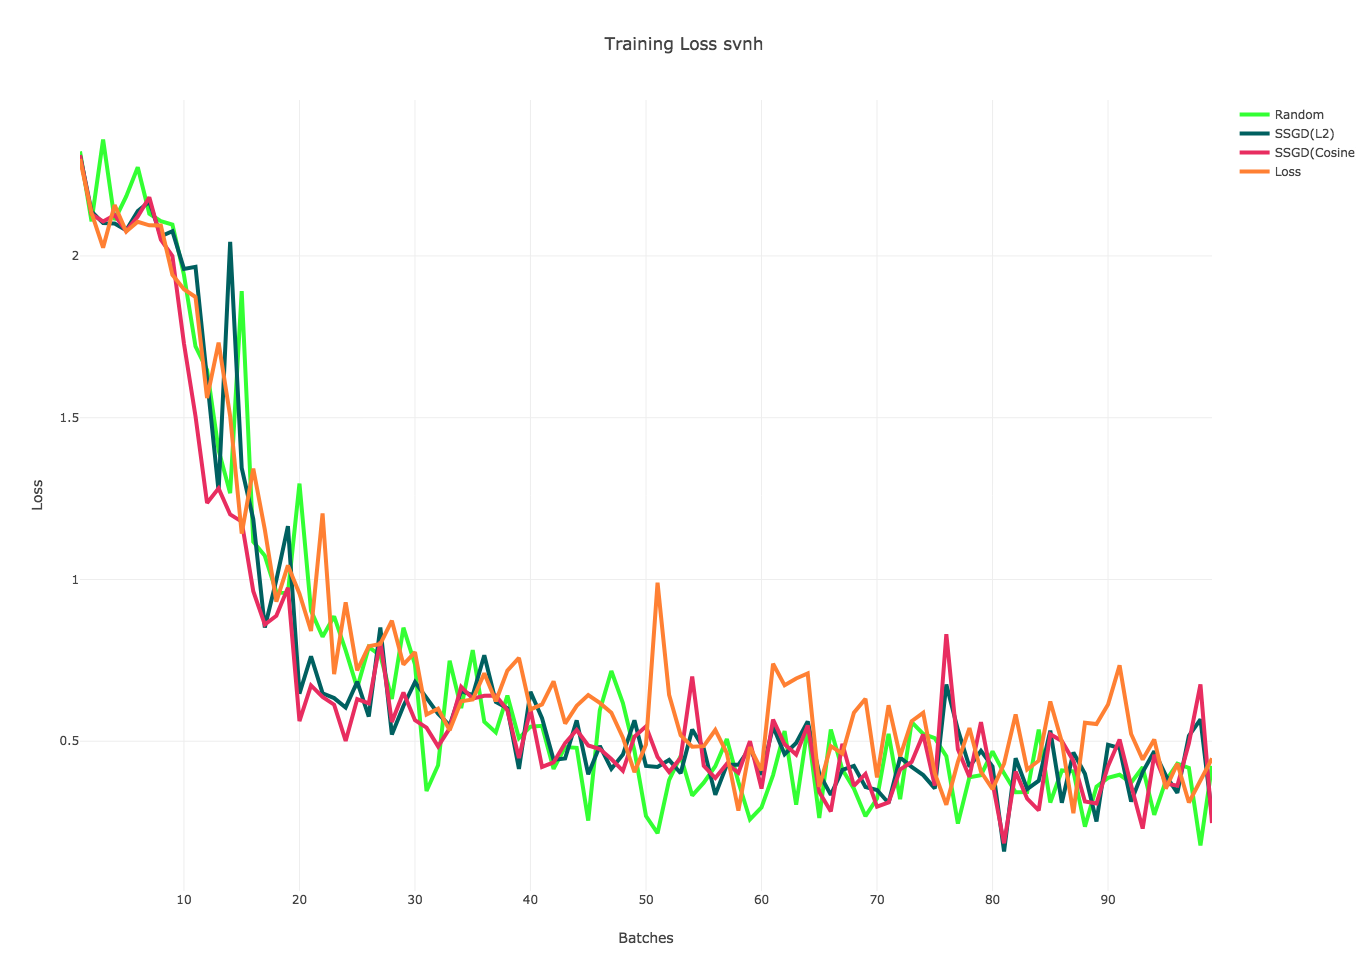
\includegraphics[width=5cm]{old/loss_svnh.png} }}%
    \subfloat[MNIST]{{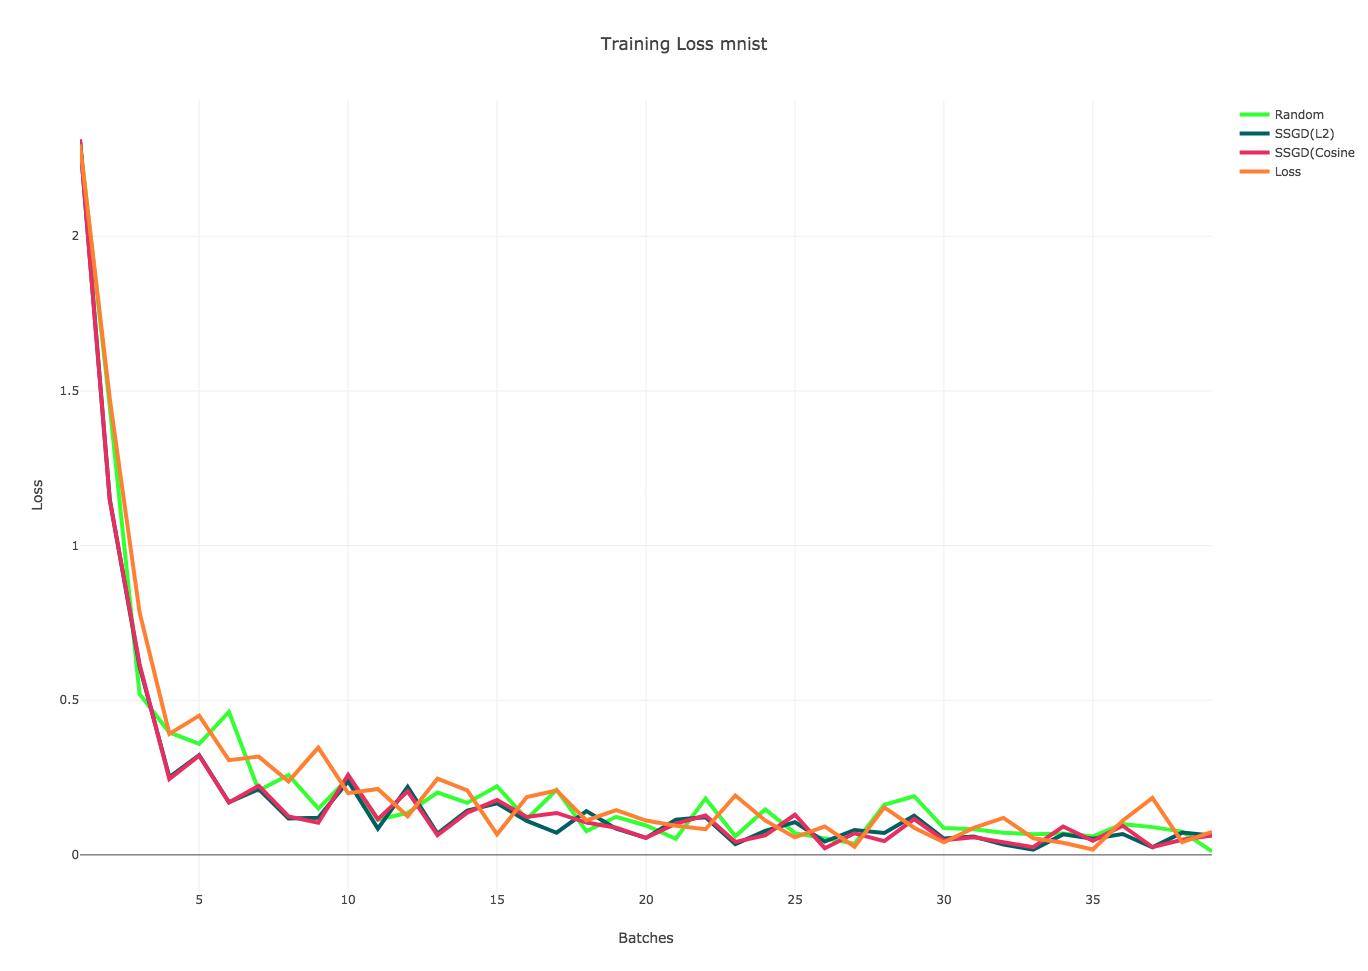
\includegraphics[width=5cm]{old/mnist_loss.png} }}%
    \subfloat[FMNIST]{{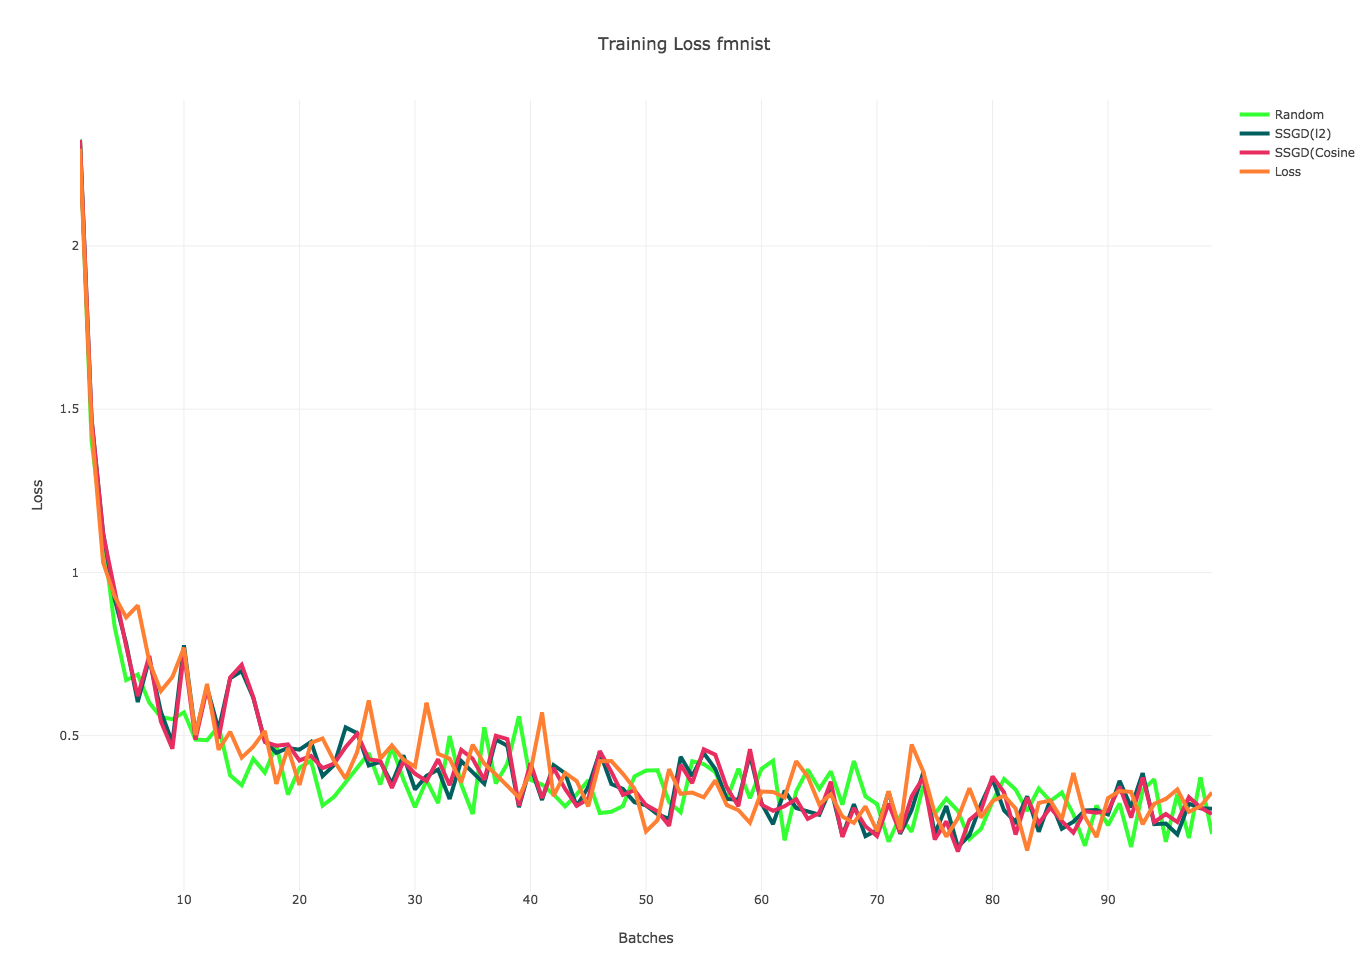
\includegraphics[width=5cm]{old/train_loss_fmnist.png} }}%
    \caption{Loss Vs Batches when using the SSGD\ref{sSGD-1} algorithm. There is no substantial  increase the speed of convergence of sgd algorithm using our method. For distance metric with ssgd we used both L2 measure and Cosine Measure.}
    \label{res-1}%
\end{figure}
\vspace{1.9pt}
We found that our algorithm discussed in \ref{sSGD-1} and \ref{sSGD-2} are comparable to both Uniform Random Sampling and Loss Based sampling as can been seen from our results \ref{res-1}
Conclusion from the above experiments:
\begin{itemize}
\item Time: For a Batch Size=64 on MNIST dataset. We need to randomly sample  940 data points 64 times for selection of 64 data points. Even with pre-computed features this causes large overhead in the selection time for data points.
\item Balanced Datasets: We also found that diversity based sampling methods does not have any significant advantage over other sampling schemes when the dataset is balanced.
\end{itemize}

For the algorithm to become more computationally efficient we propose the following changes,
\subsection{Epsilon Greedy SSGD}
\begin{algorithm}
\caption{\myalgo (eps-SSGD) Algorithm}
\label{sSGD-3}
\begin{algorithmic}[1]
\Require{Training set $X$, Model $M$, minibatch size $k$, $|X|$ = n, Fwd Batch Size L, $\epsilon$}
\Ensure{Selected a random batch R of size L}
\State $A= \phi$ \Comment \textit{Denotes set of sampled points}
\State  F $\leftarrow$ Submodular Utility function
\For{j= 0 to t} 
	\If {$\epsilon > \mathcal{U}(0, 1)$}
		\State argmax $a_j $ $\leftarrow$ $\text{argmax}_{a\in \mathbf{T}}$ $\Delta_{A_{t-1}}(a)$
      \Else
      	\State $a_j \leftarrow \mathcal{U}(1, 2, .... n)$
     \EndIf
    \State $A_{t}$ $\leftarrow$ $A_{t -1}$ $\cup$ $a_j$
\EndFor
\end{algorithmic}
\end{algorithm}
In the epsilon greedy alogrithm we first select L data points uniformly at random.
We then select k data points from these L points. Note here that we do not sample R again and again for sampling each data point. We also introduce a concept of exploration and exploitation by choosing the best data point only $\epsilon$ times and randomly selecting data points at other times.

\subsection{Adaptive Epsilon Greedy SSGD}
We can see in the previous algorithm that value of $\epsilon$ does not change but, \cite{katharopoulos2018not} suggest a adaptive value of $\epsilon$ according to Eq \ref{Fixed Eps}. We call this method the AdaptiveSSGD method.
\begin{algorithm}
\caption{\myalgo (EpsSSGDMod) Algorithm}
\label{sSGD-4}
\begin{algorithmic}[1]
\Require{Training set $X$, Model $M$, minibatch size $k$, $|X|$ = n, Fwd Batch Size L, $\epsilon$, $\alpha$}
\Ensure{Selected a random batch R of size L}
\State $A= \phi$ \Comment \textit{Denotes set of sampled points}
\State  F $\leftarrow$ Submodular Utility function
\For{j= 0 to t} 
	\If {$\epsilon > \mathcal{U}(0, 1)$}
		\State argmax $a_j $ $\leftarrow$ $\text{argmax}_{a\in \mathbf{T}}$ $\Delta_{A_{t-1}}(a)$
      \Else
      	\State $a_j \leftarrow \mathcal{U}(1, 2, .... n)$
     \EndIf
     \State Update $\epsilon$ accroding to \ref{Fixed Eps}
    \State $A_{t}$ $\leftarrow$ $A_{t -1}$ $\cup$ $a_j$
\EndFor
\end{algorithmic}
\end{algorithm}
The value of $\epsilon$ keeps on updating according to \ref{Fixed Eps}. 

\subsection{Transfer Learning on MIT67 }
We test the above stated Algorithms\ref{sSGD-4} and \ref{sSGD-3} on the task of transfer learning. Transfer learning is a very important task in the case of deep learning models. It is used when we want to use the existing features of a pre trained network to make predictions on a new dataset. \\
We fine tune a Resnet-18 convnet by freezing all but the last layer. A batch size of 16 with the forward batch size of 64 was used. The learning rate is annealed by 0.1 every 7 epochs.
The total number of training epochs is 24. For Distance calculation cosine distance between feature vectors of data points were used. 

\begin{figure}[H]
    \subfloat[Test Acc]{
    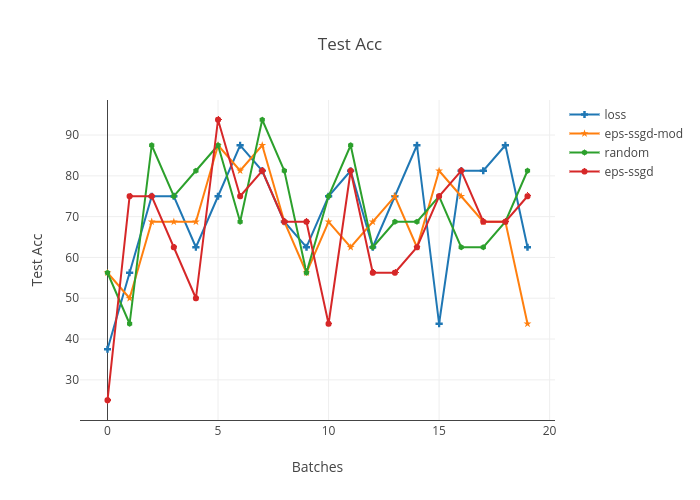
\includegraphics[width=0.5\textwidth]{transfer_learning/Test_Accplot_html.png}}%
	\subfloat[Train Loss]{
    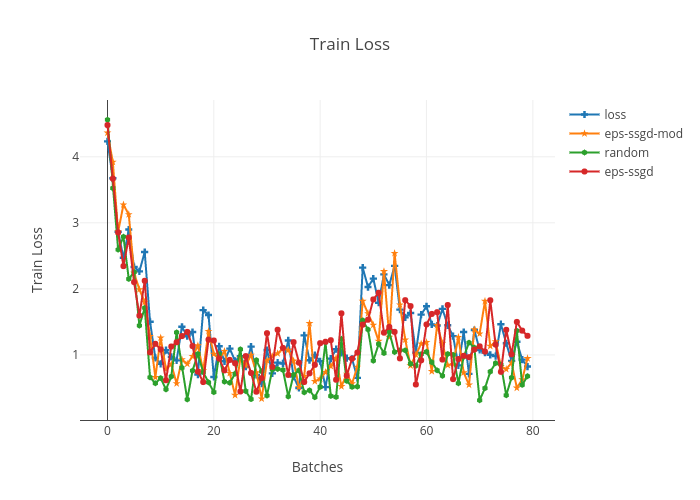
\includegraphics[width=0.5\textwidth]{transfer_learning/Train_Lossplot_html.png}}%
    \caption{(a) Test acc for random sampling is better than the our proposed method (b) Train Loss for random sampling is better than our proposed method .}
    \label{fig:Transfer learning}
\end{figure}
As we can see that on the task of transfer learning for the MIT-67 dataset random sampling performs much better than SSGD and its variants. This can primarily be attributed to the balanced nature of the dataset.

\newpage
\section{Logistic Regression on Oxford Dataset}
Our next experiment explores the need for adaptive feature vectors.
The oxford dataset is a highly imbalanced dataset and for making our task harder we used the test set for training and the training set for test making the imbalance more severe. This imbalance is pretty common place in the real world.\\ 
We used the cosine distance metric on features from a pre trained VGG-16 on the ImageNet dataset. With SGD of batch size 16 and forward batch size of 64. We annealed the learning rate after every 5 epochs by a factor of 0.1 The starting learning rate is set to 0.1. We run our experiment for 15 epochs.
\begin{figure}[H]
 \subfloat[Train Loss]{
    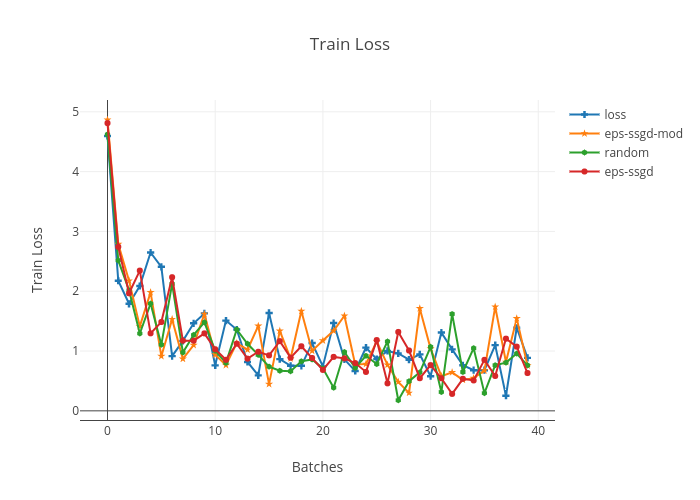
\includegraphics[width=0.5\textwidth]{oxford/oxfordTrain_Lossplot_html.png}}
    \subfloat[Train Acc]{
    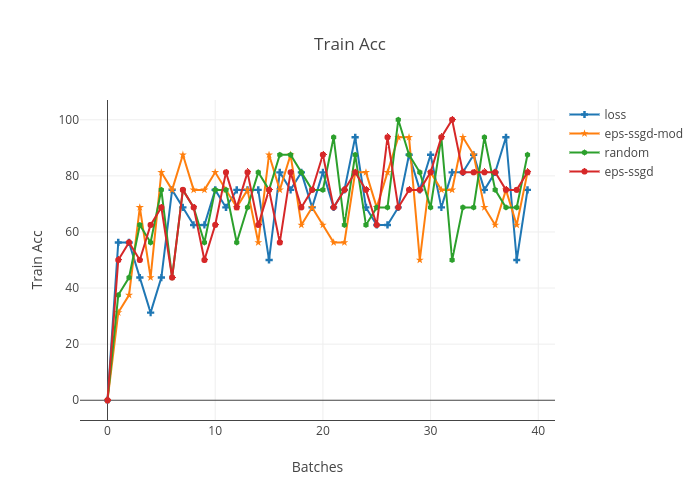
\includegraphics[width=0.5\textwidth]{oxford/oxfordTrain_Accplot_html.png}}
    \caption{Even with highly imbalanced dataset we see no major improvements with using SSGD and variants.}
    \label{fig:Oxford}
\end{figure}

If we look closely at the above graphs, we can see that SSGD and variants show much better performance on initial few batches. But after a while we can see that random sampling becomes equivalent to SSGD algorithm. This phenomena occurs because of the annealing of the learning rates, as we keep on annealing the learning rates it counters the effect of using a more diverse batch. Since a diverse batch selects data points that have the minibatch gradient approximate the true gradient much better. But a smaller learning rate actually counters this effect of the better gradient by making only small increments in the parameters updates because of a small learning rate. We explore the effect of learning rate further in \ref{Effect of learning Rate}

\subsection{Effect of $\epsilon$ value on Loss}

We experimented by tweaking the the value of $\epsilon$ in \ref{sSGD-3}. We vary the  epsilon value from 0 to 1 on both the MNIST and F-MNIST dataset. A batch size of 32 with the forward batch size of 128 was used. The learning rate was held constant at 0.01. \\

We also tested our submodular function F \ref{Entropy equation} with another standard submodular function from literature \cite{tschiatschek2016learning} called FLID function, which is also used to model diversity. We test both these function on Eps-SSGD[\ref{sSGD-3} ] algorithm. The FlID function is given by\\

\begin{equation}
f(S) = \sum_{i\in S} u_i + \sum_{d=1}^L (\text{max}_{i\in S} \space w_{i, d} - \sum_{i \in S} w_{i, d} )
\end{equation}

\begin{figure}
    \subfloat[] {{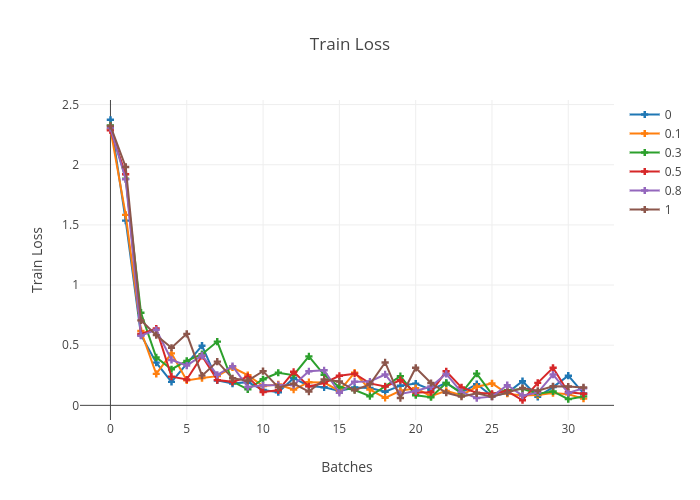
\includegraphics[width=0.25\textwidth]{eps_exp/mnistTrain_Lossssgdplot_html.png} }}%
    \subfloat[]{{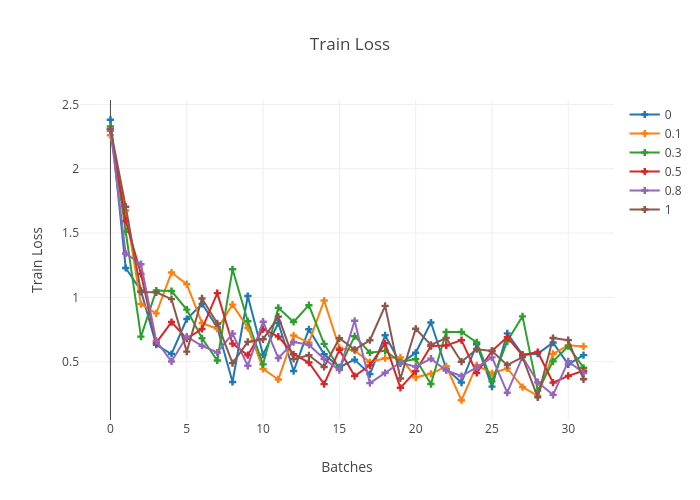
\includegraphics[width=0.25\textwidth]{eps_exp/fmnistTrain_Lossssgdplot_html.png} }}%
    \subfloat[]{{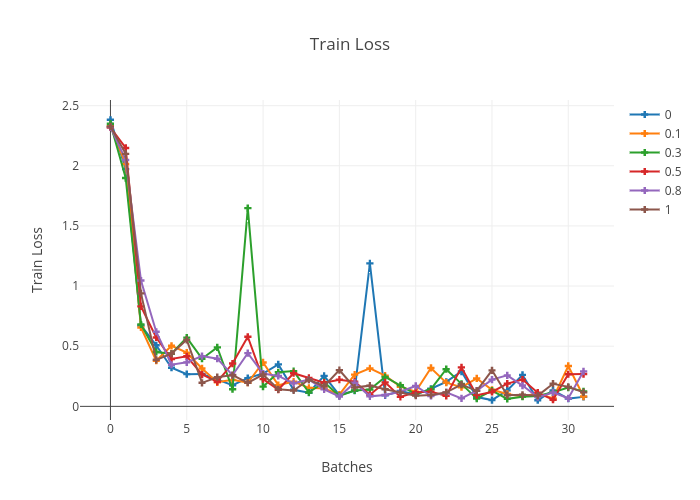
\includegraphics[width=0.25\textwidth]{eps_exp/mnistTrain_Lossdiversityplot_html.png} }}%
    \subfloat[]{{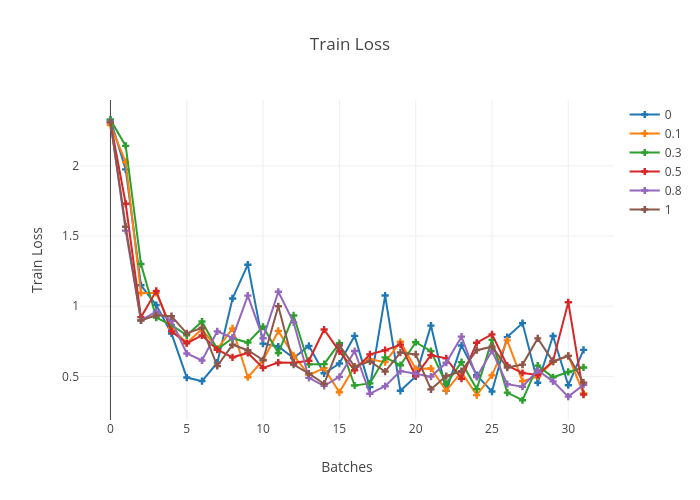
\includegraphics[width=0.25\textwidth]{eps_exp/fmnistTrain_Lossdiversityplot_html.png} }}%
    \caption{(a) \& (b) denoted the training loss using ours submodular function f \ref{Entropy equation}  on MNIST and FMNIST dataset respectively. (c) \& (d) denote the training loss using FLID function on MNIST and FMNIST dataset respectively}
    \subfloat[] {{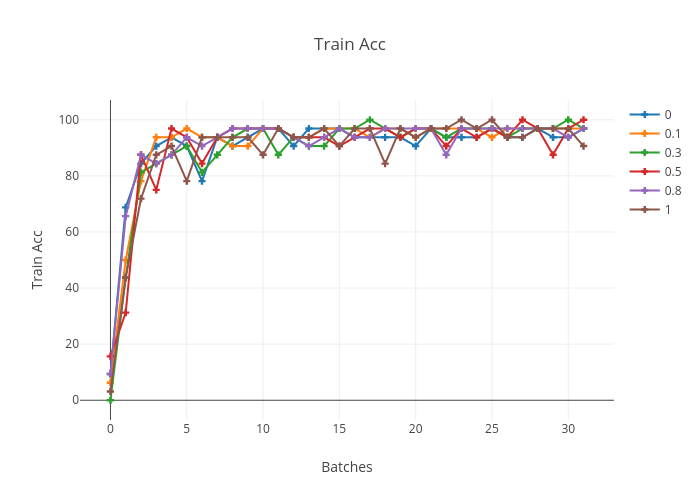
\includegraphics[width=0.25\textwidth]{eps_exp/mnistTrain_Accssgdplot_html.png} }}%
    \subfloat[]{{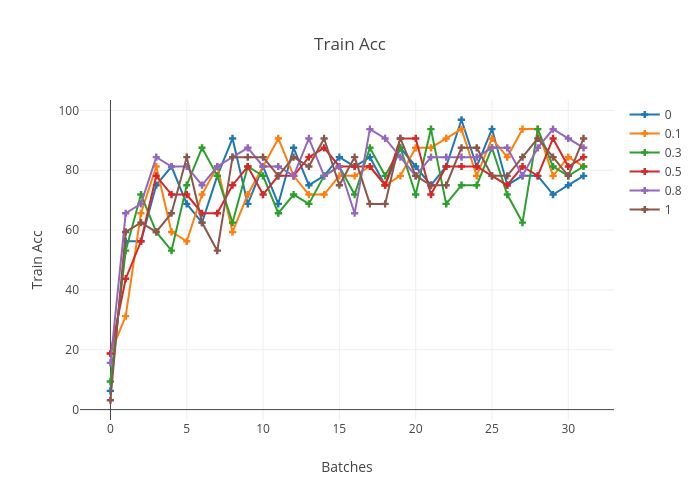
\includegraphics[width=0.25\textwidth]{eps_exp/fmnistTrain_Accssgdplot_html.png} }}%
    \subfloat[]{{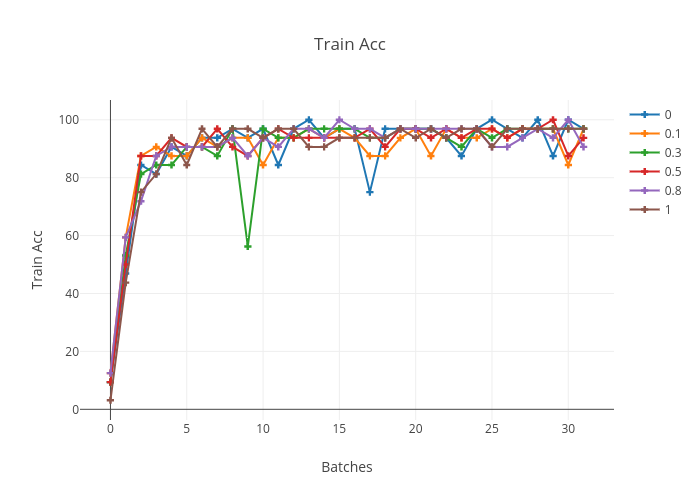
\includegraphics[width=0.25\textwidth]{eps_exp/mnistTrain_Accdiversityplot_html.png} }}%
    \subfloat[]{{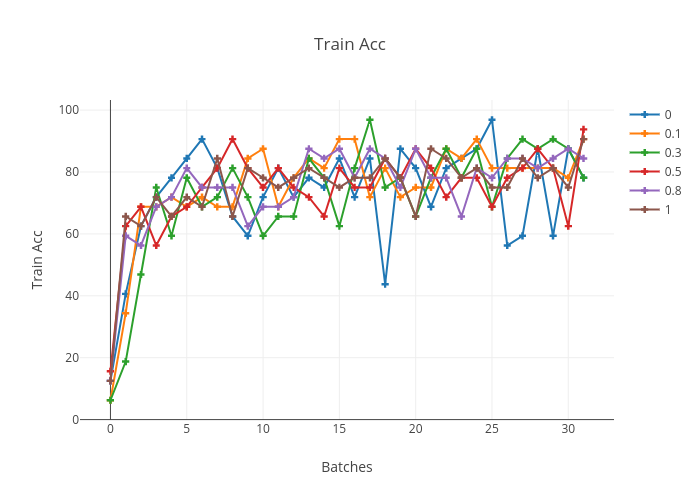
\includegraphics[width=0.25\textwidth]{eps_exp/fmnistTrain_Accdiversityplot_html.png} }}%
    \caption{(a) \& (b) denoted the training accuracy using ours submodular function f \ref{Entropy equation}  on MNIST and FMNIST dataset respectively. (c) \& (d) denote the training accuracy using FLID function on MNIST and FMNIST dataset respectively}
    \label{fig:Oxford}
\end{figure}

The FLID functions is more sensitive to the epsilon value than our function F (Eq. \ref{Entropy equation}). \\ 
The best values are 
\begin{itemize}
\item FMNIST
\begin{itemize}
\item Eps FLID: $\epsilon$=0.1(Green)
\item Eps SSGD: $\epsilon$=0.8(purple)
\end{itemize}
\item MNIST
\begin{itemize}
\item Eps FLID: $\epsilon$=1(Green)
\item Eps SSGD: $\epsilon$=0.1(yellow)
\end{itemize}
\end{itemize}
Though the best epsilon values dosen't show any important pattern but if we look more closely we see that if eps=0.1 both our function F(Eq. \ref{Entropy equation}) and FLID function perform quite well. This shows that only small degree randomness needs to introduced for the submodular sampling schemes to perform better. This can be attributed to the exploration exploitation dilemma.
\subsection{Effect of Learning Rate}\label{Effect of learning Rate}
\begin{figure}
    \subfloat[lr=0.2] {{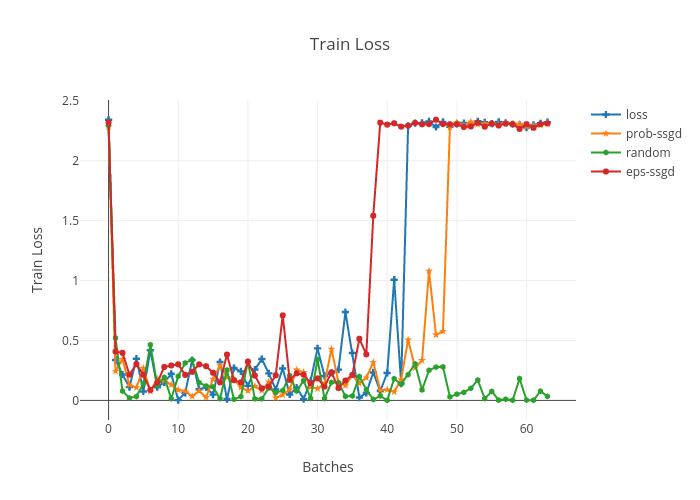
\includegraphics[width=0.20\linewidth]{learning_rate/mnistTrain_Loss0_2plot_html.png}}}%
    \subfloat[lr=0.1]{{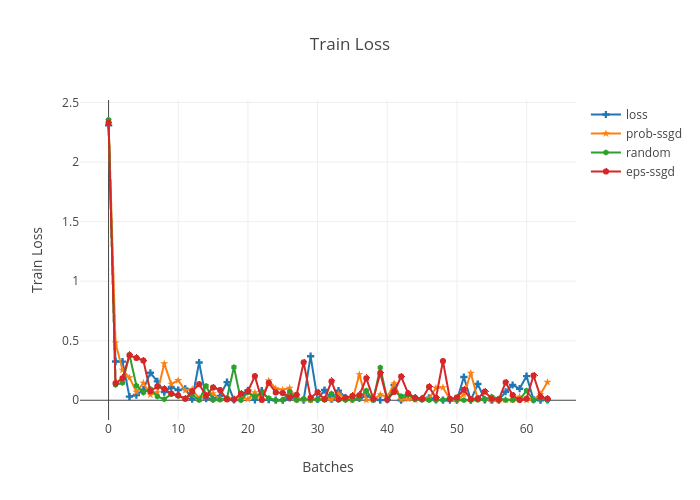
\includegraphics[width=0.20\linewidth]{learning_rate/mnistTrain_Loss0_1plot_html.png} }}%
    \subfloat[lr=0.01]{{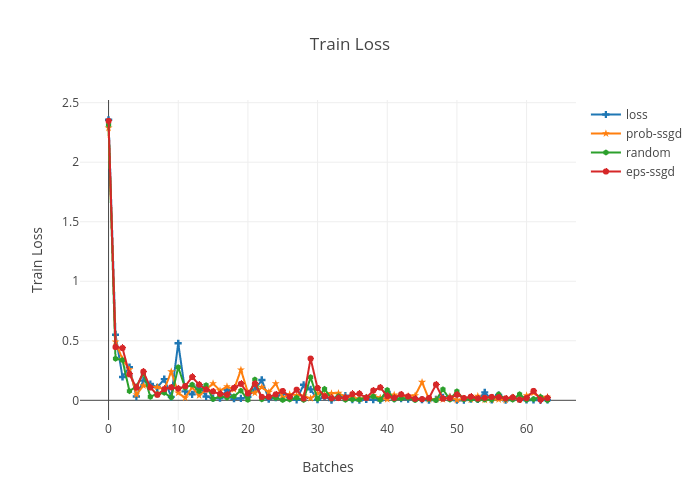
\includegraphics[width=0.20\linewidth]{learning_rate/mnistTrain_Loss0_01plot_html.png} }}%
    \subfloat[lr=0.001]{{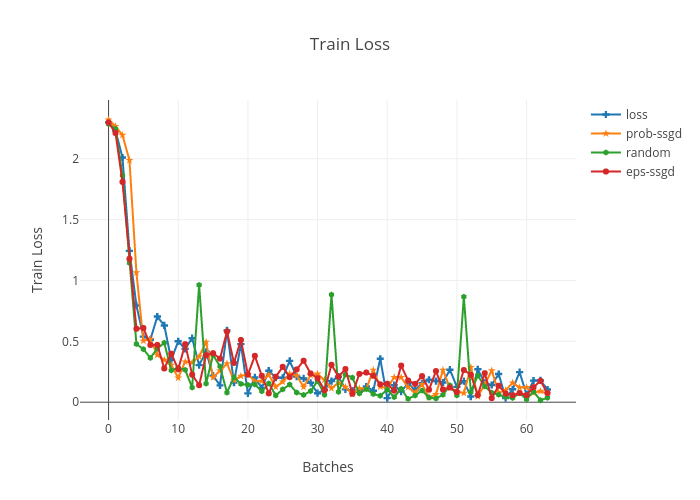
\includegraphics[width=0.20\linewidth]{learning_rate/mnistTrain_Loss0_001plot_html.png} }}%
    \subfloat[lr=0.002]{{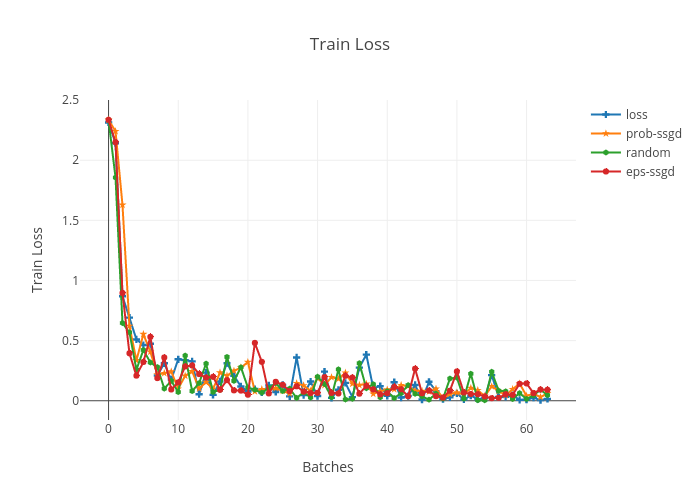
\includegraphics[width=0.20\linewidth]{learning_rate/mnistTrain_Loss0_002plot_html.png} }}%
    \caption{Training Loss with different learning rates for MNIST dataset.}
    
    \subfloat[lr=0.2] {{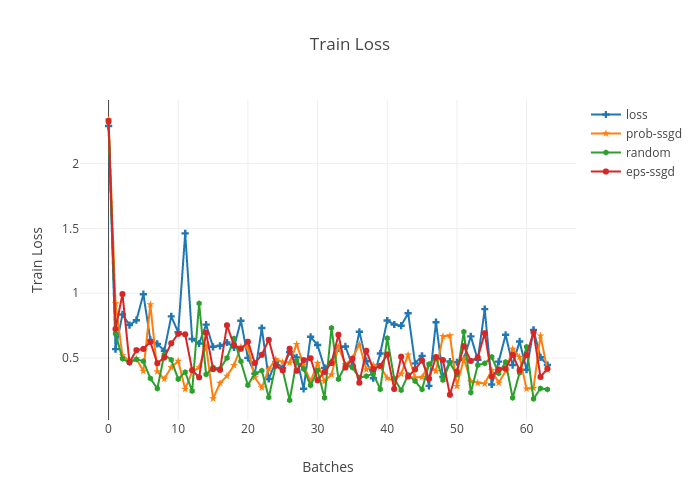
\includegraphics[width=0.20\linewidth]{learning_rate/fmnistTrain_Loss0_2plot_html.png} }}%
    \subfloat[lr=0.1]{{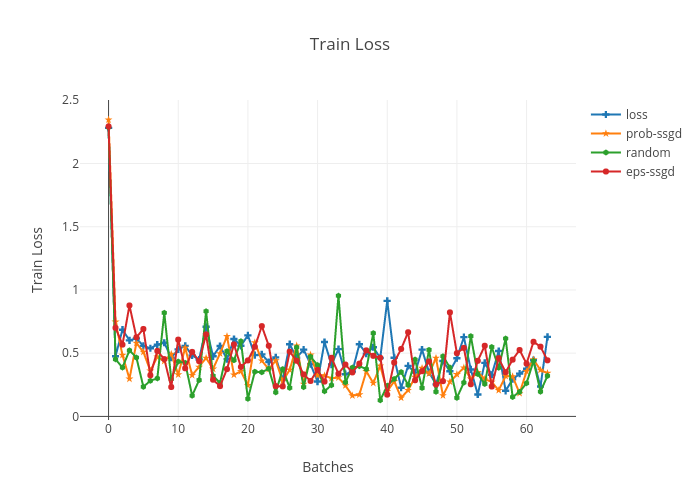
\includegraphics[width=0.20\linewidth]{learning_rate/fmnistTrain_Loss0_1plot_html.png} }}%
    \subfloat[lr=0.01]{{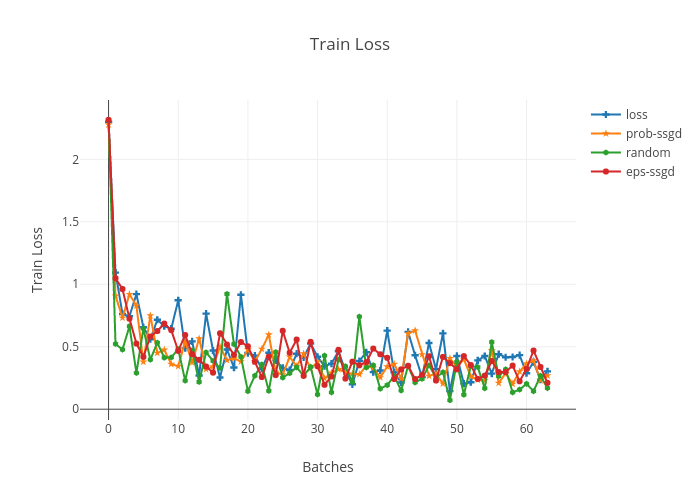
\includegraphics[width=0.20\linewidth]{learning_rate/fmnistTrain_Loss0_01plot_html.png} }}%
    \subfloat[lr=0.001]{{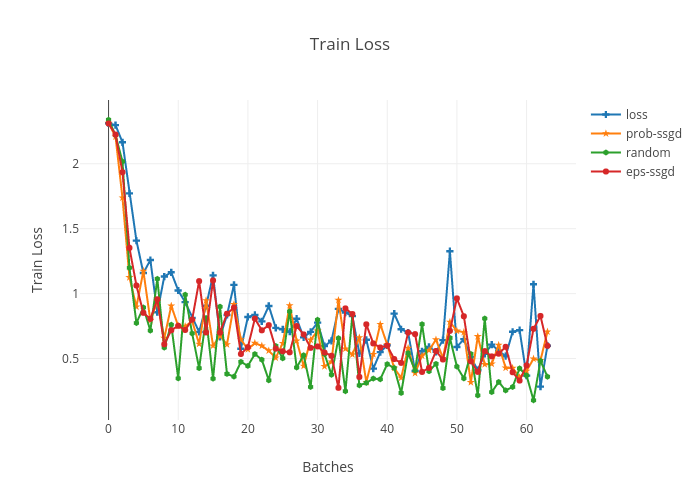
\includegraphics[width=0.20\linewidth]{learning_rate/fmnistTrain_Loss0_001plot_html.png} }}%
        \subfloat[lr=0.002]{{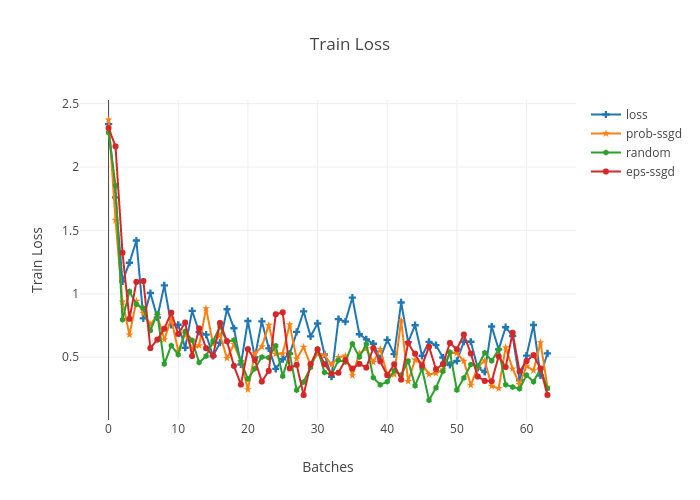
\includegraphics[width=0.20\linewidth]{learning_rate/fmnistTrain_Loss0_002plot_html.png} }}%
    \caption{Training Loss with different learning rates for FMNIST dataset.}
    \label{fig:Learning Rate Loss}
\end{figure}
\begin{figure}
    \subfloat[lr=0.2] {{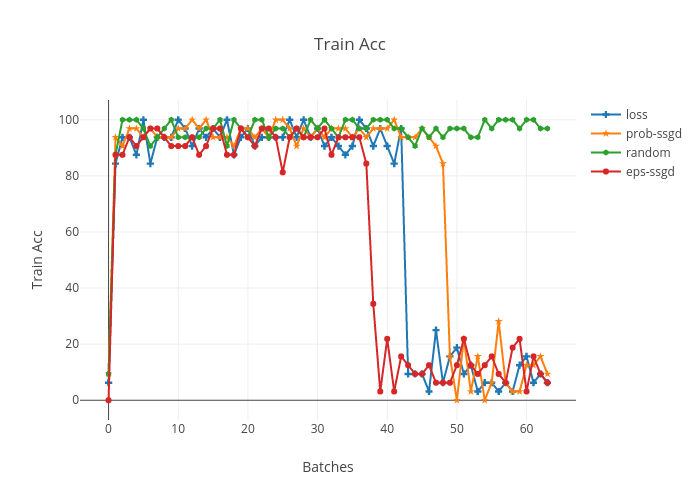
\includegraphics[width=0.20\linewidth]{learning_rate/mnistTrain_Acc0_2plot_html.png}}}%
    \subfloat[lr=0.1]{{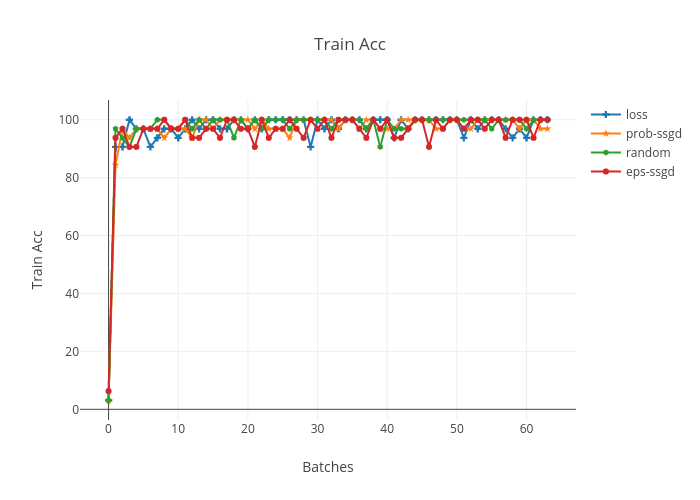
\includegraphics[width=0.20\linewidth]{learning_rate/mnistTrain_Acc0_1plot_html.png} }}%
    \subfloat[lr=0.01]{{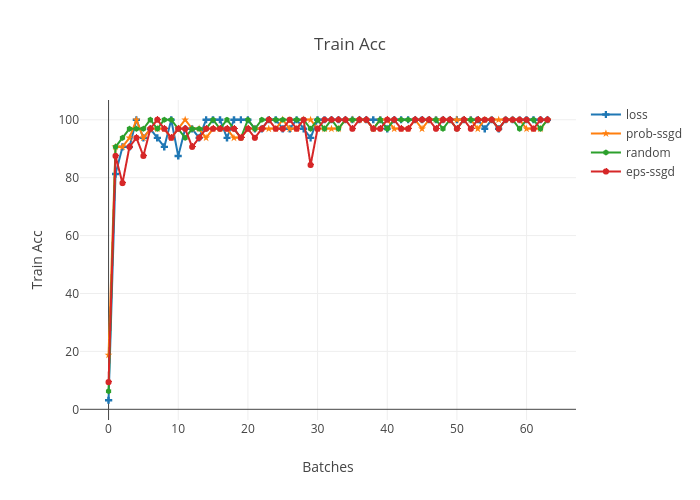
\includegraphics[width=0.20\linewidth]{learning_rate/mnistTrain_Acc0_01plot_html.png} }}%
    \subfloat[lr=0.001]{{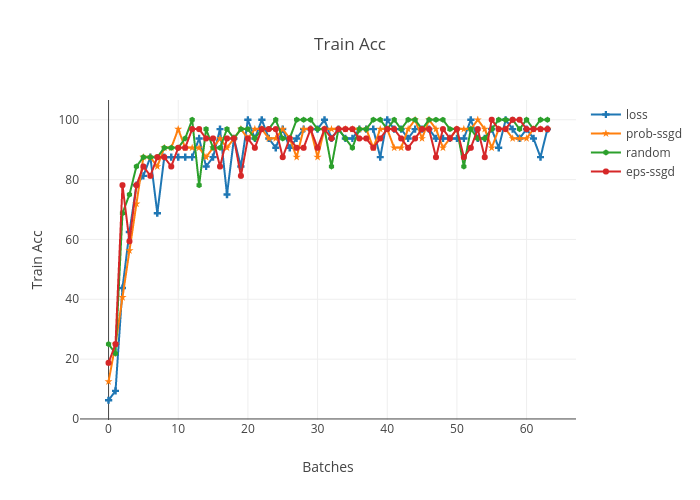
\includegraphics[width=0.20\linewidth]{learning_rate/mnistTrain_Acc0_001plot_html.png} }}%
    \subfloat[lr=0.002]{{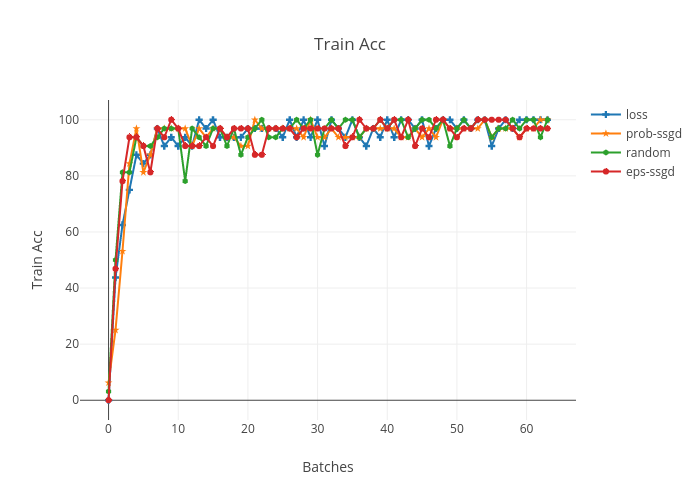
\includegraphics[width=0.20\linewidth]{learning_rate/mnistTrain_Acc0_002plot_html.png} }}%
    \caption{Training Accuracy with different learning rates for MNIST dataset.}
    \subfloat[lr=0.2] {{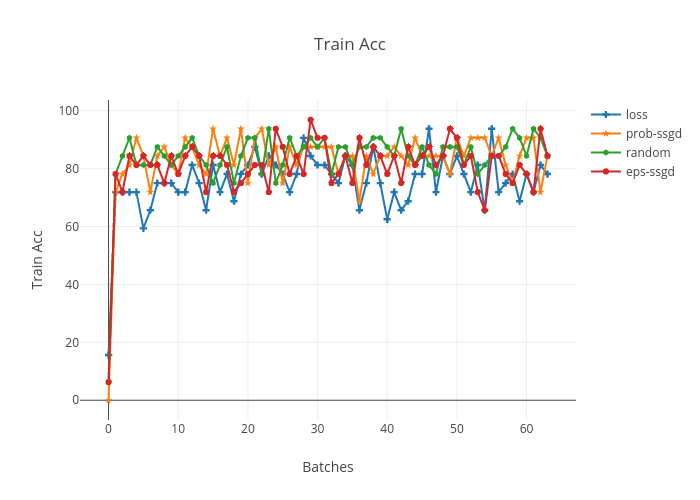
\includegraphics[width=0.20\linewidth]{learning_rate/fmnistTrain_Acc0_2plot_html.png} }}%
    \subfloat[lr=0.1]{{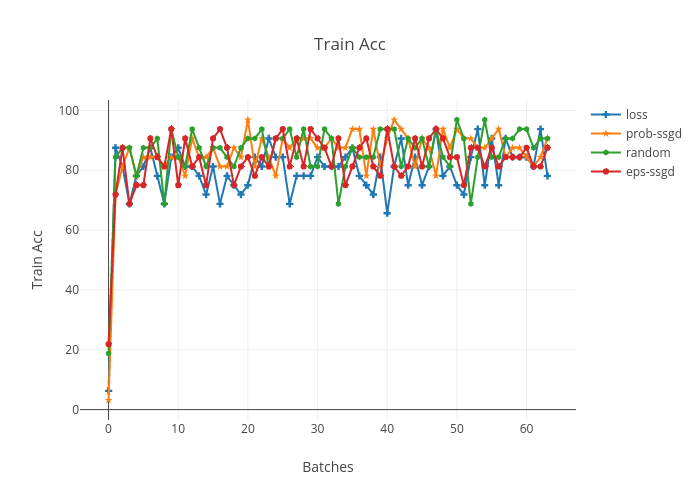
\includegraphics[width=0.20\linewidth]{learning_rate/fmnistTrain_Acc0_1plot_html.png} }}%
    \subfloat[lr=0.01]{{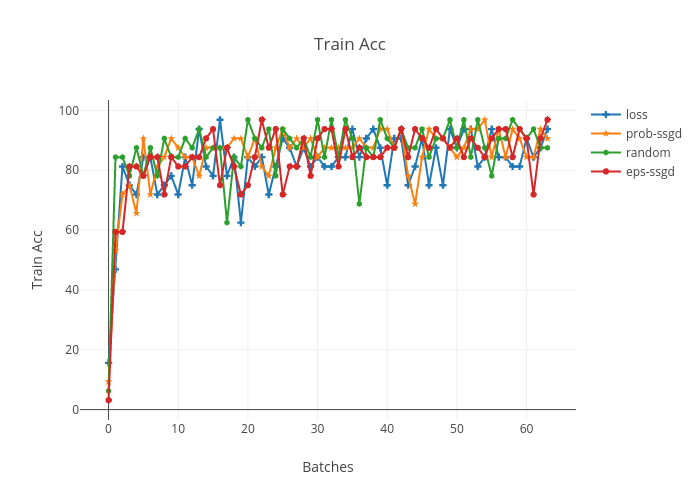
\includegraphics[width=0.20\linewidth]{learning_rate/fmnistTrain_Acc0_01plot_html.png} }}%
    \subfloat[lr=0.001]{{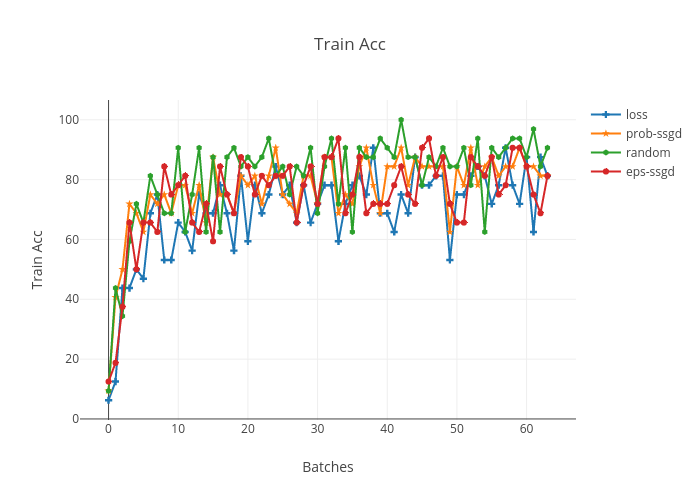
\includegraphics[width=0.20\linewidth]{learning_rate/fmnistTrain_Acc0_001plot_html.png} }}%
        \subfloat[lr=0.002]{{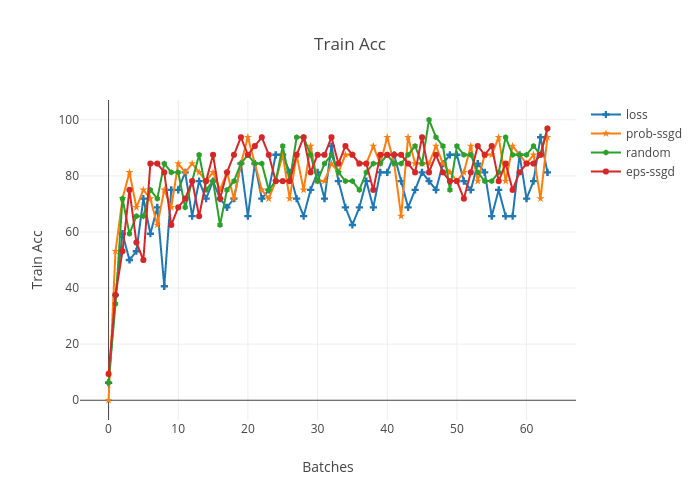
\includegraphics[width=0.20\linewidth]{learning_rate/fmnistTrain_Acc0_002plot_html.png} }}%
    \caption{Training Accuracy with different learning rates for FMNIST dataset.}
    \label{fig:Learning Rate Acc}
\end{figure}
In this experiment we test the dependence of SSGD and its variants  on the learning rate. Batch size was set to 32 and the forward batch size was set to 128 in this experiment. We trained our network for 10 epochs.
\\
This experiment confirms that our method does actually create minibatches that are diverse, since diverse minibatches also entail large gradients. We see that in Fig 10.8(a) and Fig 10.6(a) there is a problem of explosion of the gradient in the SSGD and variants. This means that gradients very very large. These large gradients can helpful for faster convergence on difficult to train dataset.
\newpage
\subsection{Imbalanced Dataset}
In this experiment we use the EMNIST dataset which consists of handwritten character digits. It contains 814,255 images with 67 imbalanced classes. We show the applicability of our method on such imbalanced datasets.
\begin{figure}[H]
\centering
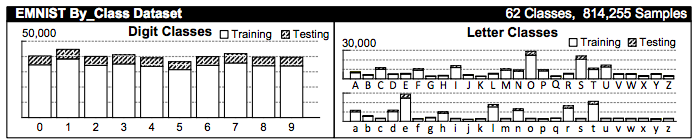
\includegraphics[width=\textwidth]{images/emnist.png}
\caption{Description of EMNIST Image}
\end{figure}
\begin{figure}[H]
    \subfloat[lr=0.2] {{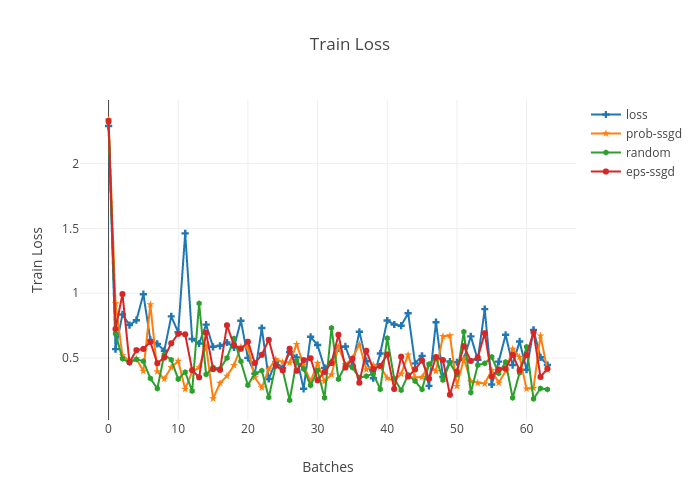
\includegraphics[width=0.20\linewidth]{learning_rate/fmnistTrain_Loss0_2plot_html.png} }}%
    \subfloat[lr=0.1]{{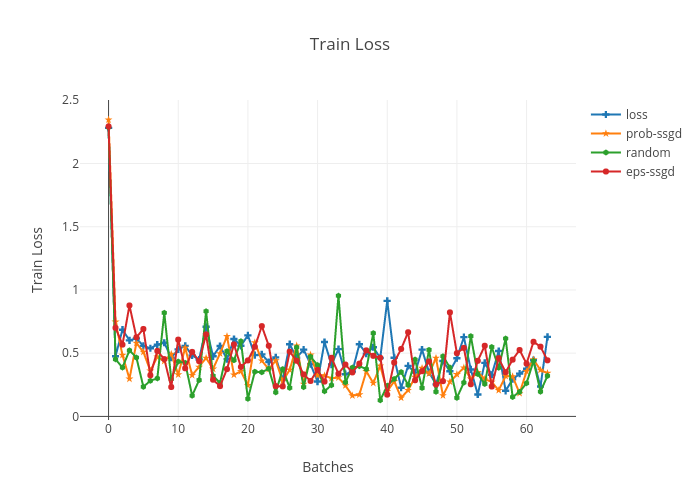
\includegraphics[width=0.20\linewidth]{learning_rate/fmnistTrain_Loss0_1plot_html.png} }}%
    \subfloat[lr=0.01]{{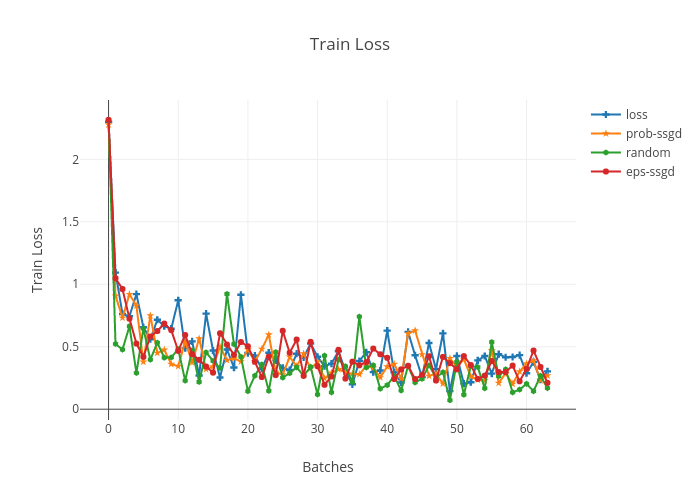
\includegraphics[width=0.20\linewidth]{learning_rate/fmnistTrain_Loss0_01plot_html.png} }}%
    \subfloat[lr=0.001]{{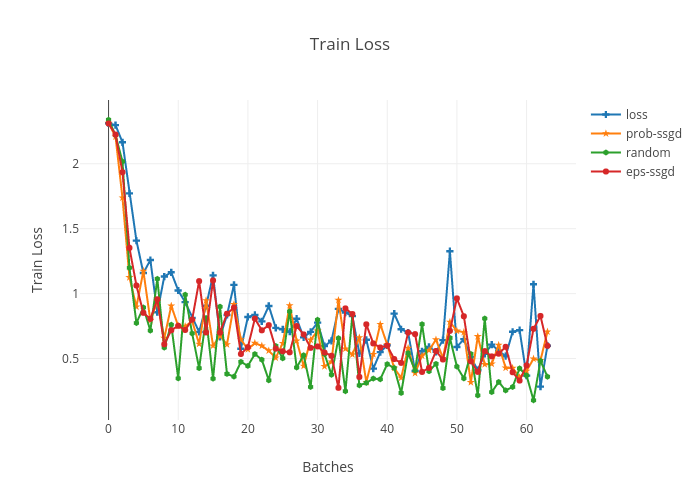
\includegraphics[width=0.20\linewidth]{learning_rate/fmnistTrain_Loss0_001plot_html.png} }}%
        \subfloat[lr=0.002]{{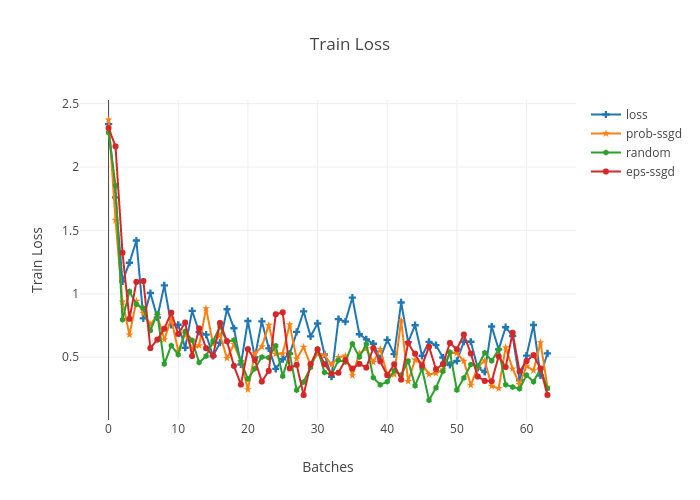
\includegraphics[width=0.20\linewidth]{learning_rate/fmnistTrain_Loss0_002plot_html.png} }}%
    \caption{Training Loss with different learning rates for EMNIST dataset.}
    \subfloat[lr=0.2] {{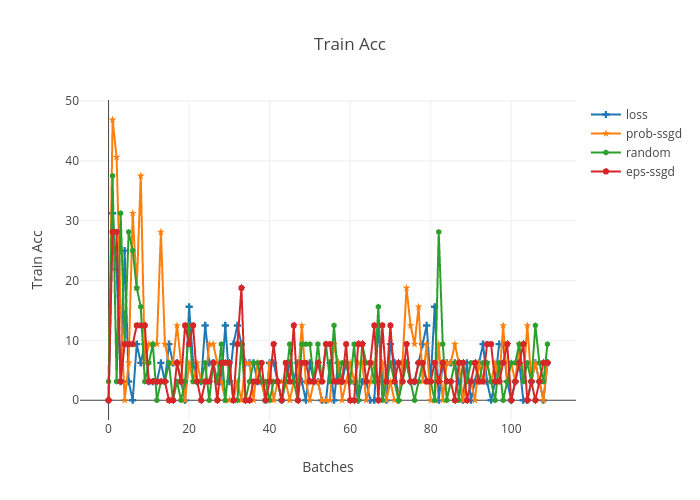
\includegraphics[width=0.20\linewidth]{learning_rate/emnistTrain_Acc0_2plot_html.png}}}%
    \subfloat[lr=0.1]{{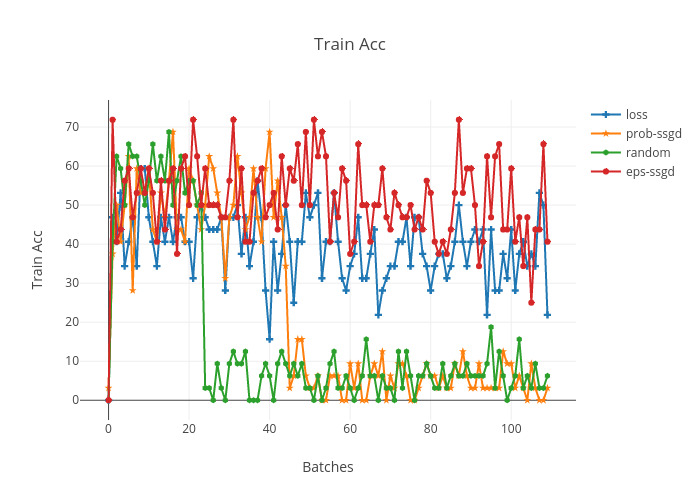
\includegraphics[width=0.20\linewidth]{learning_rate/emnistTrain_Acc0_1plot_html.png} }}%
    \subfloat[lr=0.01]{{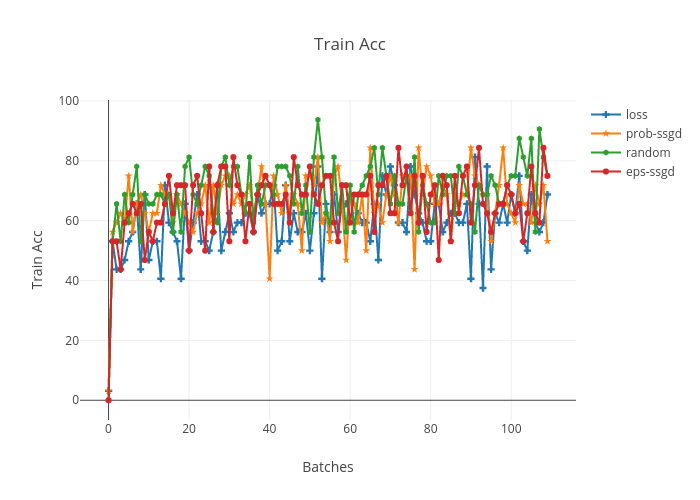
\includegraphics[width=0.20\linewidth]{learning_rate/emnistTrain_Acc0_01plot_html.png} }}%
    \subfloat[lr=0.001]{{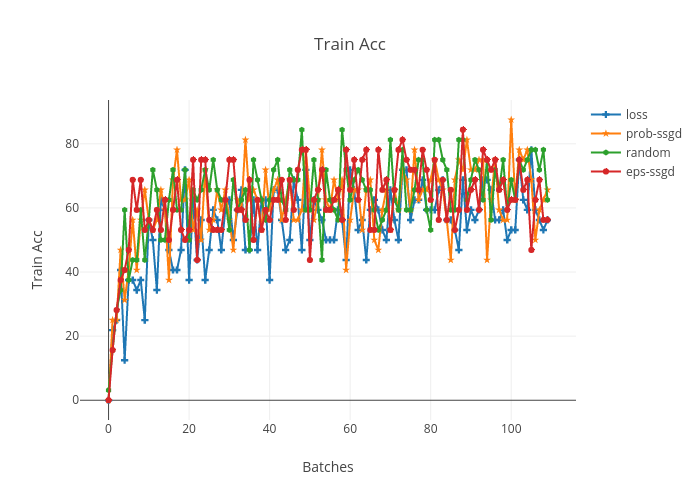
\includegraphics[width=0.20\linewidth]{learning_rate/emnistTrain_Acc0_001plot_html.png} }}%
    \subfloat[lr=0.002]{{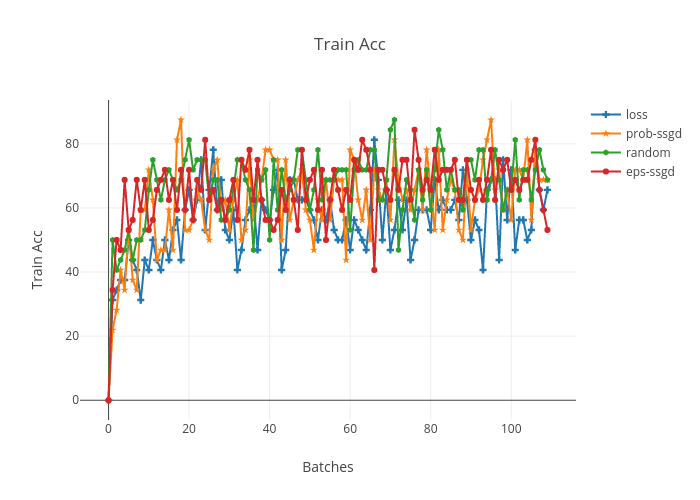
\includegraphics[width=0.20\linewidth]{learning_rate/emnistTrain_Acc0_002plot_html.png} }}%
    \caption{Training Accuracy with different learning rates for EMNIST dataset.}
    \label{fig:Emnist Learning Rate Loss}
\end{figure}
Imbalanced datasets are hard to train on and particular care should be taken about the learning rate parameter for these datasets. We see in Fig 10.11(a) and Fig 10.12(a) that for a learning rate of 0.2 all the algorithms failed. But the interesting case was for the learning rate of 0.1. As we can see that Eps-SSGD performs really well when a learning rate of 0.1 was used but random sampling fails to learn with that learning rate. This shows us that our algorithm can outperfom random sampling with the correctly tuned learning rate.
\newpage
\subsection{Effect of Batch Ratio}
Since we modified the Lazier than Lazy greedy algorithm by selecting k samples from set of randomly sampled set of points of size B rather than selecting only one data point, we investigate the effect of batch ratio on the algorithm.
We define Batch Ratio(BR)=$\frac{k}{B}$. We test both \ref{sSGD-1} and \ref{sSGD-2} algorithms on the FMNIST and MNIST dataset.
\begin{figure}
\subfloat[]{{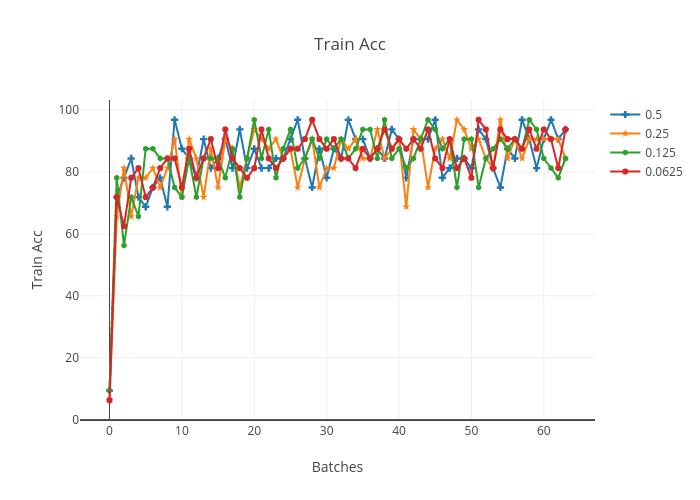
\includegraphics[width=0.5\linewidth]{batch_ratio/fmnistTrain_Accssgdplot_html.png}}}%
\subfloat[]{{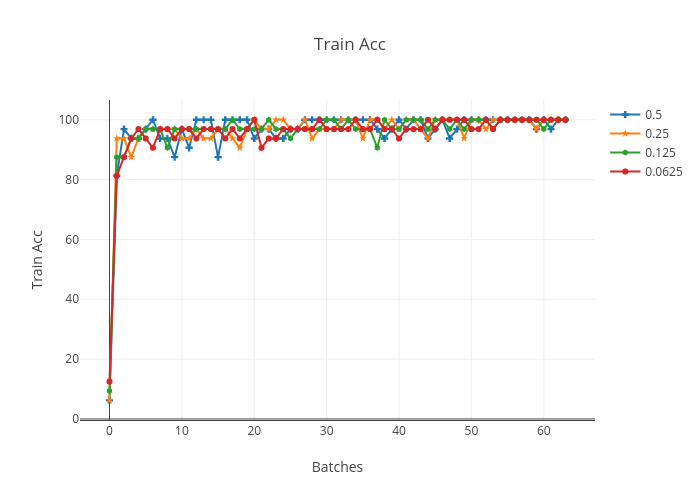
\includegraphics[width=0.5\linewidth]{batch_ratio/mnistTrain_Accssgdplot_html.png}}}%

\caption{Training loss (a) FMNIST (b) MNIST with different batch sizes on Eps-SSGD}
\subfloat[]{{\includegraphics[width=0.5\linewidth]{batch_ratio/fmnistTrain_Lossssgdplot_html.png}}}%
\subfloat[]{{\includegraphics[width=0.5\linewidth]{batch_ratio/mnistTrain_Lossssgdplot_html.png}}}%
    \caption{Training Acc (a) FMNIST (b) MNIST with different batch sizes with Eps-SSGD }
    \label{fig:Emnist Learning Rate Loss}
\end{figure}
We now investigate batch ratios effect on \ref{sSGD-4} algorithm
\begin{figure}
\subfloat[] {{\includegraphics[width=0.5\linewidth]{batch_ratio/fmnistTrain_Accprob-ssgdplot_html.png}}}%
\subfloat[]{{\includegraphics[width=0.5\linewidth]{batch_ratio/mnistTrain_Accprob-ssgdplot_html.png}}}%

\caption{Training Loss (a) FMNIST (b) MNIST with different batch sizes with Eps-SSGD-Mod }
\subfloat[]{{\includegraphics[width=0.5\linewidth]{batch_ratio/fmnistTrain_Lossprob-ssgdplot_html.png}}}%
\subfloat[]{{\includegraphics[width=0.5\linewidth]{batch_ratio/mnistTrain_Lossprob-ssgdplot_html.png}}}%
    \caption{Training Acc (a) FMNIST (b) MNIST with different batch sizes with Eps-SSGD-Mod}
    \label{fig:Emnist Learning Rate Loss}
\end{figure}

The results of these experiment are really interesting as it shows that there is not much correlation between batch ratio and the convergence of SSGD this is rather strange as it is orthogonal to the theoretical results in \cite{mirzasoleiman2015lazier}. We leave the exploration of the theoretical consequence of this experiment as a future work.
\newpage
\subsection{Results on Cifar10}
The CIFAR-10 dataset consists of 60000 32x32 colour images in 10 classes, with 6000 images per class. There are 50000 training images and 10000 test images. We train a VGG-11 network using a batch size of 16 with a forward batch size of 64. We used a constant learning rate of 0.1 and trained the network for 60 epochs.
\\
\begin{figure}
\subfloat[] {{\includegraphics[width=0.5\linewidth]{cifar-10/cifarTrain_Loss11plot_html.png}}}%
\subfloat[]{{\includegraphics[width=0.5\linewidth]{cifar-10/cifarTest_Acc11plot_html.png}}}%
\caption{(a) Training Loss of cifar-10 (b) Test Accuracy of cifar-10 dataset}
\label{cifar-10}
\end{figure}
We see that on a hard to train dataset like Cifar-10, our algorithm performs much better than both random and loss based sampling. In this example random sampling fails completely learning nothing this can be attributed to not tuning the learning rate for SGD.

\subsection{Effect of Depth}
\begin{figure}
\subfloat[]{{\includegraphics[width=0.5\linewidth]{cifar-10/cifarTrain_Loss13plot_html.png}}}%
\subfloat[]{{\includegraphics[width=0.5\linewidth]{cifar-10/cifarTest_Acc13plot_html.png}}}%
\caption{(a) Training Loss of cifar-10 (b) Test Accuracy of cifar-10 dataset for VGG-13}
\subfloat[] {{\includegraphics[width=0.5\linewidth]{cifar-10/cifarTrain_Loss16plot_html.png}}}%
\subfloat[]{{\includegraphics[width=0.5\linewidth]{cifar-10/cifarTest_Acc16plot_html.png}}}%
\caption{(a) Training Loss of cifar-10 (b) Test Accuracy of cifar-10 dataset for VGG-16}
\label{cifar-10}
\end{figure}
As the depth on the network increases surprisingly random sampling starts to learn again this can be attributed to smoother loss landspace with deeper networks but even with deeper depths SSGD and its variants perform much better both on the train and test dataset.
\newpage
\section{Time Analysis}
We now show the avg time per epochs for all tasks stated above. The standard SSGD
\begin{table}[!htb]\label{Dataset}
	\renewcommand{\arraystretch}{1.5}
	\centering
	\begin{tabular}{|c|c|c|c|c|c|} \hline
		\textbf{Task} & \textbf{Random} & \textbf{Loss} & \textbf{SSGD} & \textbf{ProbSSGD} & \textbf{ProbSSGD-Mod}\\ \hline
		Transfer Learning & $\approx$ 10  &  $\approx$ 13 & - & $\approx$ 22 & $\approx$ 20\\ \hline
		Logistic Regression & $\approx$ 2   &  $\approx$ 9.6 & - & $\approx$ 4.6 & $\approx$ 2.4 \\ \hline
        Cifar-11 & $\approx$ 2.44  &  $\approx$ 5.18 & $\approx$ 6.53 & $\approx$ 6.59 & $\approx$ 7.108 \\ \hline
		Cifar-13 & $\approx$  3.84 &  $\approx$ 6.81 & - & $\approx$ 9.05 & $\approx$ 7.82 \\ \hline
		Cifar-16 & $\approx$ 4.26 & $\approx$ 5.91 & - & $\approx$ 6.42 & $\approx$ 8.61\\ 
\hline
	\end{tabular}
    \caption{Avg time per epoch in each of the tasks in min.}
\end{table}

As we can see that SSGD and its variants are really slow as compared to random sampling. This heavily outweighs the benefits of using SSGD and variants. We need to come up with a better engineering solution for making submodular sampling more time efficient. This time analysis does not show the full picture though because SSGD and its variant train the neural network in much lesser epochs than random sampling for datasets like Cifar-10.

\chapter{Conclusion and Future Work}

In this work, we presented a novel framework to sample a diverse  minibatch at each iteration for  faster convergence of SGD algorithm. We argue that modeling diversity is an NP hard problem but can be solved easily if we use submodular functions. We introduced a novel submodular function and a several new submoudular optimization techniques for scaling to large dataset. Our submodular optimsation methods reduces variance in SGD in a provable manner. We applied our framework on different datasets and different tasks like transfer learning, Logistic Regression, Image Classification etc and extensively studied the effects of parameters such as learning rate, batch ratio, epsilon on the performance of our algorithm. 
The main contribution of our work is showing both empirically and theoretically that diversity based sampling for minibatch creation can lead variance reduction in SGD. Which in turn leads to faster convergence of SGD algorithms. \\
Although our algorithm works comparable to random sampling on many datasets such as FMNIST and MNIST we show that in the case of CIFAR-10 dataset our algorithms outperforms random and loss based sampling by huge margins. We also show that for imbalanced dataset if we tune the learning rate correctly we can see faster convergence of SGD using our algorithm. Another interesting result of our work was disproving the bounds in \cite{mirzasoleiman2015lazier}, we showed that the dependency on batch ratio is not that critical. Our algorithm is much slower in terms of wall clock time as compared to the random sampling algorithm and we need to find better engineering solutions to this problem. Below we list a few possible directions to make our algorithms faster,
\begin{itemize}
\item Instead of assigning scores to each data points, assigns probabilities to each subset using Probabilistic Submodular Functions.
\item Use of distributed submodular maximization algorithms. These algorithms are really fast and have provable bounds for accuracy of the results.
\end{itemize}
One area which is still left unexplored is the usage of our algorithm in the setting Natural Language Processing and Multi task training. This is an really interesting setting since submodular functions have been extensively used in both these areas. A diverse batch would really be useful in the case of multi task learning as the batch would now be contain information from all tasks leading to better models being trained. We leave the exploration of these task as a future work.
\clearpage
\newpage
\addcontentsline{toc}{chapter}{References} % Please do not remove this
\bibliographystyle{iiththesis.bst}
\bibliography{sofc}
\end{document}
\documentclass[a4paper,twoside]{iiththesis}
\usepackage[margin=1in]{geometry}
\usepackage{graphicx}
\usepackage[lofdepth,lotdepth]{subfig}
\usepackage{algorithm}
\usepackage{algpseudocode}
\usepackage{amsmath, amssymb}
\usepackage{xcolor}
\usepackage{float}

\usepackage{xspace}
\usepackage{subfig}
\usepackage[english]{babel}
\renewcommand{\algorithmicrequire}{\textbf{Input:}}
\renewcommand{\algorithmicensure}{\textbf{Output:}}
\usepackage{times}
\usepackage{amsthm}
\usepackage{amsfonts}
\usepackage{amssymb}
\usepackage{enumitem}
\usepackage{lipsum}
\usepackage{fixltx2e}
\usepackage{parskip}

\newcommand{\squeezeup}{\vspace{-2.5mm}}
\newtheorem{theorem}{Theorem}
\theoremstyle{definition}
\newtheorem{definition}{Definition}[section]
\theoremstyle{definition}
\newtheorem{claim}{Claim}[section]
\newcommand{\myalgo}{Submodular-SGD\xspace}
\newtheorem{prop}{Proposition}
\addcontentsline{toc}{chapter}{References} % Please do not remove this
 
\theoremstyle{remark}
\newtheorem*{remark}{Remark}
\DeclareMathOperator*{\E}{\mathop{\mathbb{E}}}

\usepackage{graphicx}
\book{Thesis}
\title{Submodular Importance Sampling for Neural Network Training}
\degree{Master of Technology}
\department{Computer Science}
\submitted{June 2018}
\author{Krishna Kant Singh}
\adviser{Dr Vineeth N Balasubramanian}
\addradviser{Dept. of Computer Science \\ IITH}
\chair{---------}
\addrchair{Dept. of Computer Science \\ IITH}
\external{----------}
\addrexternal{Dept. of Computer Science \\ IITH}
\internal{----------}
\addrinternal{Dept. of Computer Science \\ IITH}
\coguide{----------}
\addrcoguide{Dept. of Computer Science \\ IITH}

\acknowledgements{Firstly, I would like to thank my thesis advisor, Dr. Vineeth N Balasubramanian for introducing me to the field of Machine Learning. I thank him for his helpful discussion and patience which helped me a lot. Next, I want to thank Dr. Naveen Sivadasan whom I worked with on the problem of Sub-Graph classification. It was a joy to work with him. I also want to extend a thank you to Dr Kotaro Kataoka how actually helped a lot during my initial research period. I would like to express my constant gratitude to Dept of Computer Science IIT Hyderabad for providing the motivation and resources to help me in successfully completing my work. I am also thankful to my seniors and friends for their friendly advice and words of encouragement in the due course of my research. I would like to especially thank Krutika Verma for helpful conversation and clearing a lot my doubts. Finally I want to thank my family without whom none of this was possible. }

\abstract{
Stochastic Gradient Descent(SGD) algorithms are the workhorse on which Deep Learning systems have been built upon. The standard approach of uniform sampling in SGD algorithm leads to high variance between the calculated gradient and the true gradient, consequently resulting in longer training times.\\
Importance sampling methods are used for sampling mini-batches that reduce this variance. There exist provable importance sampling techniques for variance reduction but,they generally do not fare well in the case of Deep Learning models. \\\\
Our work proposes sampling strategies that create diverse mini-batches which consequently leads to the reduction in the variance of the SGD algorithm.
We pose the task of creation of such mini-batches as, maximization of a submodular objective function. The proposed submodular objective function samples minibatches that such that more uncertain and diverse set of samples are selected with high probability. \\\\
Submodular functions can be optimized easily using the GREEDY\cite{nemhauser} algorithm but, even the newer variants suffer from performance issues when the size of the dataset is large. We propose a new faster submodular optimization method method which is inspired from \cite{mirzasoleiman2015lazier}.
\\ \\
We prove theoretically that our sampling scheme reduces variance in the case of SGD algorithm. We also show that Determinantal point process(DPP) sampling can also be seen as a special case of our algorithm.
\\ \\
We showcase the generalization of our method by testing it on several deep learning data sets like MNIST,FMNIST, CIFAR-10 datasets.
We study the effect of learning rate, network architecture etc on our proposed method.We study how different features affect the performance of our algorithm.
We also study the case of transfer learning with our algorithm used for selection of the dataset. In all the experiments, we compare our algorithm with Loss based sampling and Random sampling for comparison.
}


\renewcommand{\bibname}{References}
\begin{document}

\part{Introduction}
\chapter{Introduction and Motivation}

Stochastic Gradient Descent(SGD) methods are one of the main reasons for the success of Deep Learning. With the availability of "Big-Data" stochastic methods have proven to be the most effective methods for training Deep Neural Networks. \\ \\ 
In machine learning we are interested in minimizing the loss function generally of the form,
\begin{equation*}
    F(\theta) = \textbf{argmin} \frac{1}{N} \sum_{i=1}^N  f(x_i; \theta)
\end{equation*}
Typically, f is convex and denotes the misfit between the i-th training instance and its corresponding target.
% * <vineethnb@iith.ac.in> 2018-03-04T12:19:03.867Z:
% 
% > Typically, each $f(i; \theta)$ is convex
% Is this correct?
% 
% ^ <krishnakant.singh@suiit.ac.in> 2018-06-17T13:16:42.633Z.
The training data is represented as ${x_i, y_i}$ and N denotes the total number of data points.
A typical way of solving these optimization problems is through gradient descent algorithms,
\begin{align}
\begin{split}
    \theta_{t+1}&=\theta_{t} - \eta \frac{1}{N}\sum_{i=1}^N \nabla( ; \theta_t)\\
                            &\eta: \text{learning rate}\\
                            & \nabla(; \theta_t) = \sum_{i=1}^N\nabla(f(x_i; \theta_{t}))
      \end{split}
\end{align}
The above formulation requires gradients for each of the N data points, which is prohibitively expensive even for a small N. SGD provides a solution to above problem where the parameter update is conditioned upon only a  single  data point selected uniformly at random
\begin{align}
\begin{split}
    &\theta_{t+1}=\theta_{t} -  \eta  \nabla(x_i, \theta_t) \\
\end{split}   
\end{align}
    
It can be shown that $\nabla(x_i, \theta_t)$ is an unbiased estimate of the full batch gradient $\nabla (:, \theta_t)$ , $\E (\nabla( x_i, \theta_t)) = \frac{1}{N}\sum_{i=1}^N \nabla f(x_i; \theta_t)$ but, SGD introduces high variance between the estimated gradient $\nabla(x_i, \theta_t)$ and the true gradient $\nabla(; \theta_t)$ , due to this reason stochastic gradients methods have a much slower convergence.  A simple way of reducing the variance is to use mini-batch SGD. 
\begin{align}
\begin{split}
    &\theta_{t+1}=\theta_{t} -  \frac{1}{k}\eta  \sum_{i=1}^k \nabla (x_i, \theta_t) \\
    & k: \text{batch size}
   \end{split}
\end{align}
\\ 
\section{Importance Sampling}
Creation of a minibatch which is representative of the full data set can help in reducing the variance due to the stochastic sampling. Higher importance should be given to data points that provide the most information to the network, in literature this called as hard example mining\cite{shrivastava2016training}.  This way of choosing the data points is also popularly called Importance Sampling.  % * <vineethnb@iith.ac.in> 2018-03-04T13:38:10.150Z:
% 
% > \begin{align*}
% >     \theta^+= \theta-\sum_{i=1}^B \frac{1}{B} \nabla(f(x_i; \theta))\\
% > \end{align*}
% Generally, the 1/B is outside the summation (although this is not wrong)
% 
% ^ <krishnakant.singh@suiit.ac.in> 2018-06-22T12:42:50.086Z.

In standard SGD full gradient is approximated using a Monte Carlo estimate given by
\begin{align}
\tilde{\nabla}(f(; \theta_t)) & = \frac{1}{B}\sum_{i=1}^B p(x_i) \nabla(f(x_i; \theta_t))\\
& = E_{p(x)}\nabla(f(x_i; \theta_t)
\end{align}
Here $p(x)$ denotes the sampling distribution that is used for selecting B data points ie , $P(x=x_i) = p(x=x_i) = \frac{1}{B}$ \\
This approximation can be improved using Importance Sampling as follows
\begin{align}\label{imp-sample}
\begin{split}
	\tilde{\nabla}(f(; \theta_t)) & = \frac{1}{B}\sum_{i=1}^B p(x_i) \nabla(f(x_i; \theta_t))\\
    \tilde{\nabla}(f(; \theta_t)) & = \frac{1}{B}\sum_{i=1}^B \frac{p(x_i)}{q(x_i)} q(x_i) \nabla(f(x_i; \theta_t))\\
    \tilde{\nabla}(f(; \theta_t)) & = E_{q(x)}\left( \frac{p(x_i)}{q(x_i)}  \nabla(f(x_i; \theta_t))\right)\\
 \end{split}
\end{align}
Here q(x) denotes the surrogate sampling distribution, that is used for selecting B data points ie , $P(x=x_i) = q(x=x_i)$ \\
In chapter 3 we show that if q(x) is chosen appropriately, is an unbiased estimator. Also, we prove that using importance sampling leads to variance reduction. 
% * <vineethnb@iith.ac.in> 2018-03-04T13:40:10.975Z:
% 
% > \begin{align*}
% >     \theta^+&=\theta-\sum_{i=1}^B q(x) \frac{p(x)}{q(x)} \nabla(f(x_i; \theta))\\
% >             &\text{where} \hspace{0.2em} x_i \in q(x)
% > \end{align*}
% What is x? x may need to be defined, to make this equation well-defined.
% 
% ^ <krishnakant.singh@suiit.ac.in> 2018-06-22T13:31:28.757Z.
\section{Importance Sampled SGD}
For importance sampling based SGD we can write the update rule as follows, 
% * <vineethnb@iith.ac.in> 2018-03-04T12:19:27.453Z:
% 
% > Higher importance should be given to data points that provide more information to the model. 
% It's not clear why choosing most informative points should reduce variance. If we are showing this later, we may have to rephrase this accordingly.
% 
% ^ <krishnakant.singh@suiit.ac.in> 2018-06-17T13:17:55.764Z.
\begin{align}
\begin{split}
    \theta_{t+1} &=\theta_t - \eta \sum_{i=1}^N w_{I_t} \nabla(f(x_{I_t}; \theta_t))\\ 
    &= \theta_t - E_{p(x)} (w_{I_t} \nabla(f(x_{I_t}; \theta_t))\\
\end{split}
\end{align}
The probability of sampling a data point $x_i$ is given by $P (x = x_{I_t}) = p^t (x_i)$. We can see that p(x) is adaptive and changes at each iteration t, $w_{I_t}$ denotes the rescaling coefficients for $x_{I_t}$.
% * <vineethnb@iith.ac.in> 2018-03-04T12:20:11.491Z:
% 
% > \begin{align*}
% >     \theta^+&=\theta-\sum_{i=1}^B p(x) \nabla(f(x_i; \theta))\\
% >             &\text{where} \hspace{0.2em} x_i \in q(x)
% > \end{align*}
% This doesn't seem complete?  P(x) needs to add upto 1? How do you define q(x)?
% 
% ^ <krishnakant.singh@suiit.ac.in> 2018-06-22T12:43:06.597Z.
The above reduces to standard SGD if $w_{I_t} = 1$ and $p^t(x_i) = \frac{1}{N}$
\begin{align}
    \theta_{t+1}= \theta_t- \frac{\eta}{N} \sum_{i=1}^N  \nabla(f(x_{I_t}; \theta_t))\\
\end{align}

Some known strategies for importance sampling in SGD are to sample data points proportional to the loss, or to gradients of the parameters. Sampling with respect to gradients is essentially a case of hard example mining. \\
The drawback with gradient based sampling is that it requires the full gradient and is sensitive to outliers. Moreover, mini-batches should not only consist of the most informative data points but also points that are diverse enough to represent the full data set for eg it is better to include data points from all classes rather than just one class. This becomes much more important in the case of imbalanced datasets. \\
\section{Diversity}\label{diversity_explained}
The diversity of mini-batch is an important quality for circumventing bias in mini-batches. A popular method for modeling diversity in literature is to use Submodular Functions. A submodular functions is defined as ,\\
A function $f:2^V\longrightarrow R$ is submodular if for any A$\subseteq$ B $\subseteq$ V, and v $\in$ V/B,we have that:
    \begin{equation*}
        f(A\cup v) - f(A)\geq f(B\cup v)- f(B)    
    \end{equation*}
using this definition we can  see that submodular functions  are good candidates for modeling diversity. The above property is popularly known as the diminishing return property. Submodular function are ideally suited for selection of a diverse set of data points. Also, submodular function are easy to maximize as they just require the greedy solution at each step which makes their optimization fast. 

Another  popular approach for modeling diversity is Deterministic Point Process(DPP) which use a similarity kernel $\mathbf{L}^{N \times N}$ , $\mathbf{L}_{ij}$ denoting the similarity between data points i and j for sampling diverse data points. \\
The DPP assigns a probability of sub sampling any subset Y $\subseteq \{1,...,N\}$, proportional to the determinant of the sub-matrix $\mathbf{L_Y}$ of   $\mathbf{L}$, 
\begin{equation} \label{dpp_eq}
P(Y) = \frac{\text{det}(\mathbf{L}_Y )} { \text{det}(\mathbf{L}+I)} \propto \text{det}(\mathbf{L}_Y)
\end{equation}
For instance, if $Y$ consists of only two elements i and j,
then P(Y) $\propto \mathbf{L}_{ii} \mathbf{L}_{jj} - \mathbf{L}_{ij}\mathbf{L}_{ji}$ where $\mathbf{L}_{ij}$ and $\mathbf{L}_{ji}$ measure the similarity between elements i and j, being more similar lowers the probability of co-occurrence. On the other hand, a diverse subset has a higher value of the determinant. Thus, DPP naturally favours a diversified selection of subsets. \\

DPP and other similar models come under the class of functions called Probabilistic Submodular Functions(PSF). A major problem in using DPP for minibatch selection is that sampling from a DPP is an expensive operation it scales polynomially with number of data points size $O(N^3)$. \\
Thus, a need arises for methods that model diversity as well as DPP but, are much easier to sample from.  Another, issue with DPP is that it is hard to always define a meaningful similarity kernels for datasets. 
\\
\\
The main contributions of our work are as following 
\begin{itemize}
    \item Designing a sampling scheme that encodes both importance of sample and diversity for the creation of representative batches for the whole data set.
    \item Constructing a method for scalable optimization of submodular objective function, thus enabling their use in the era of Big Data. 
    \item We prove that our method is an unbiased estimator for the full gradient and that it reduces variance in SGD and SGD-Type algorithms.
    \item Our designed approach leads to faster convergence and higher classification accuracy in image classification task. Out methods is also more robust to the hyperparameters such as learning rate and minibatch size. 
\end{itemize}

As far as we know our work is one of the first to use submodular functions for importance sampling in the context of variance reduction in SGD. Also, we are one of first papers that perform large-scale importance sampling based image classification task on datasets such as cifar-10 and MIT-67 datasets.

\part{Prerequisites }

\chapter{Deep Neural Networks and Stochastic Gradient Descent}
In this chapter we first give a brief overview of Neural Networks and Deep Learning. We then show how the Backpropogation algorithm along with SGD(Stochastic Gradient Descent) is used to train a neural network.
\\\\
Machine learning is commonly divided into two main types:
\begin{itemize}
\item Supervised Learning: These methods try to learn a hypothesis $\mathcal{H} : X \rightarrow Y$ which maps the input data domain to the output data domain as well as possible. If the output set Y is finite, we say that the task is a classification task and if it is continuous we say that it is a regression task.
\item Unsupervised Learning: If all we have is the input data X and no output data to guide our training, the task is called unsupervised learning. The focus in this type of learning is
to discover hidden structure in the data. Common problems in unsupervised learning are dimensionality reduction and clustering of the input data.
\end{itemize}

Recently deep Learning has revolutionized the field of both supervised 
and Unsupervised Learning. Tasks which once seemed impossible to be done by a machine are now being excelled at . ImageNet Classification challenge which sparked the boom for the Deep Learning Research, is now a solved problem with the machines achieving super-human level of accuracies on the task. \\ \\
Though deep learning methods still suffer from some huge problems like, 
\begin{itemize}
\item Large Dataset: Deep Learning Networks require huge amounts of data to trained. It is not always possible to have acess to such data. There is a need for algorithms that train faster and better using only a small subset of data.
\item Performance on Imbalanced datasets: Deep learning system generally perform poorly on imbalanced datasets, this is due to the fact that the network is unable to learn classes/events which occur very sparsely in the dataset.
\end{itemize}
Our work tries to mitigate both of the above points through the use importance sampling for training of Deep Neural Networks.

In the next section we derive the now popular back propagation algorithm used to train neural networks. \\
\section{Neural Network}\footnote{\label{NN}In this section subscript$_i$  denotes  denotes i th dimension. But everywhere else subscript$_i$  denotes i th data point}
\begin{figure}[!htb]
\centering
\includegraphics[width=0.5\textwidth]{images/nn.png}
\caption{A one layer NN network}
\label{Simple NN}
\end{figure}
We take a Neural Network (NN) as shown in fig \ref{Simple NN}} with the following parameters, 
\begin{itemize} 
\item Input vector of length of K, $x = (x_1, x_2, x_3, ....., x_K)$. 
\item Hidden layer consists of N neurons $h = (h_1, h_2, h_3, ....., h_N)$. 
\item Ouput layer is of size M, $\textbf{y} = (y_1, y_2, y_3,...., y_M)$. 
\end{itemize}
Every neuron in the input layer is connected to all the neurons in the hidden layer, the connection weight between neuron i and k is given by $w_{ki}$. Similarly, all the neurons in the hidden layer are connected to the output layer, the connection weight between the ith hidden neuron and j th output neuron is given by $w_{ij}'$.\\
We can think of $w_{ki}$ as the k,i entry in the matrix $\mathbf{W}^{K \times N}$, similarly $w_{ij}'$ can be considered as the i,j entry in the $\mathbf{W}^{K \times N}'$,. The activation function f is the sigmoid activation function.
\\ 
\\
\textbf{Forward Pass}
The forward pass can be expressed by the following equations, 
\begin{align}
&h_i = f(u_i) = f(\sum_{k=1}^K w_{ki} x_k) \hspace{0.8pt} [\text{This is the ouput of the i th neuron in the hidden layer }] \\
&y_j=f(u_{j}^{'})=f(\sum_{i=1}^K w_{ij}^{'} h_i) \hspace{0.8pt} [ \text{This is the ouput of the j th neuron in the ouput layer} ] \\
&\text{if we assume a Mean Squared Error Loss} \\
&E(x) = \frac{1}{2} \sum_{j=1}^M (y_j - t_j)^2
\end{align}
\newpage
\textbf{Backward Pass}\\
In the backward pass we compute the loss and gradient of loss wrt(with respect to) to all the parameters($\mathbf{W}$) in the NN. We the pass these gradient back and update the parameters of the network.
\begin{align}
&\frac{\partial E(x) }{w_{ij}^{'}} = \frac{\partial E(x)}{\partial{y_j}} \frac{\partial{y_j}}{\partial{u_{j}'}}\frac{\partial u_{j}'}{w_{ij}'}\\
&\frac{\partial E(x)}{\partial{y_j}} = \sum_{i=1}^M (y_{j} - t_{j}) \\
&\frac{\partial{y_j}}{\partial{u_{j}'}} = y_j (1-y_j) \\
&\frac{\partial u_{j}'}{w_{ij}'} = h_i
\end{align}
Hence, 
\begin{align}
&\frac{\partial E (x)}{w_{ij}^{'}} = \sum_{i=1}^M (y_j - t_j) y_j (1 - y_j) h_i
\end{align}
Similarly we can get, \begin{align}
\frac{\partial E(x)}{w_{ki}} = \frac{\partial E}{\partial y_j}\frac{\partial y_j}{\partial u_{j}'}\frac{\partial u_{j}'}{\partial h_i}\frac{\partial h_i}{\partial u_i}\frac{\partial u_i}{\partial w_{ki}}
\end{align}

This is the famous Backpropogation algorithm it is so called, because we are back propagating the gradients from output to the input.\\
The update rule for parameters  is given by 
\begin{align}
w_{ij}'^{+} = w'_{ij} - \eta * \frac{\partial E(x) }{w_{ij}'}
\end{align}
where $\eta$ denotes the learning rate. \\
\subsection{Gradient Descent }
Back propagation only computes the gradient for only one sample, in practice back propagation is generally combined with learning algorithms such as gradient descent which computes the gradient for all the samples in the training data. Hence, Gradient Descent update rule is given by 
\begin{align}
w_{ij}'^+ = w_{ij}' - \frac{\eta}{N} \sum_{x}  \frac{\partial E(x) }{w_{ij}'}
\end{align}
For ease of discussion we now employ the following convection for parameter updates 
\begin{align}
\theta_{t+1} = \theta_{t} - \frac{\eta}{N} \sum_{i=1}^N \nabla(f(x_i; \theta_t))
\end{align}
Here f denotes the Loss function and $x_i$ denotes the i th point in the dataset $\mathcal{D}$ of size N . We can see that computing the gradient  for all of the N data points is computationally expensive. In practice only a part of dataset is used for computing the gradient and  updating of the parameters in one iteration. \\
\subsection{Stochastic Gradient Descent (SGD)}
The stochastic gradient estimates the true gradient on the whole dataset by using only a single data point. The update rule for the SGD algorithm is given by 
\begin{align}
\theta_{t+1} = \theta_{t} - \eta \nabla(f(x_i; \theta_t)) \label{SGD}
\end{align}
We can show that the stochastic gradient  $\nabla(f(x_i; \theta_t)$ is an unbiased estimate of the true gradient $\nabla(f(; \theta_t)$, if we assume that the samples are iid (independent identically distributed) and we choose any point uniformly at random then, 
\begin{align}
E(\nabla(f(x_i; \theta_t))) = \frac{1}{N} \sum_{i=1}^N \nabla(f(x_i; \theta_t) 
\end{align}
This shows that the stochastic gradient estimate is unbiased, but the variance of stochastic gradient algorithm is non-zero as shown below , \\
Using Taylor Series and assuming that f is an L-smooth function we get
\begin{align}
\E f(x; \theta_{t+1}) &\leq \space  \E f(x; \theta_t) - \eta \E \big(\nabla f(x, \theta)^T (\theta_{t+1} - \theta_{t})\big) - \frac{L\eta^2}{2} \E || (\theta_{t+1} - \theta_{t}) || ^2 \\
& \leq \E f(x; \theta_t) - \eta ||\E \nabla  f(x; \theta_{t})||^2 - \frac{L\eta^2}{2} \E ||t\nabla f(x; \theta_{t})||^2  \hspace{1.2pt} \text{[Using Eq \ref{SGD}]} \\ 
&\leq \E f(x; \theta_t) - \eta ||\E \nabla f(; \theta_{t})||^2 - \frac{L\eta^2}{2} \E\Big[ \nabla f(x; \theta_{t})^2\Big] \\
&\leq \E f(x; \theta_t) - \eta(1 -\frac{L\eta}{2}) ||\E \nabla f(; \theta_{t})||^2 + \frac{L\eta^2}{2}  \mathbb{V}(\nabla f(x ;\theta)) \label{Variance Red}
\end{align}
Where , $\mathbb{V}(\nabla f(x; \theta)) = \E || \nabla f(x; \theta) - \E\nabla f(x; \theta)||^2 $.\\\\
From the above Eq \ref{Variance Red} it can be easily seen that a smaller variance helps in getting to a better optimal solution faster.\\ In the next chapter we see some popular techniques in literature that have been used for variance reduction.

\chapter{Variance Reduction Techniques}

Variance Reduction\footnote{The major Source of this chapter is Handbook of Monte Carlo Methods} is an important part of many approximation algorithms like SGD@. These techniques help in finding a more precise approximation quantity of intreset resulting in a better performance models that are being trained using these approximation algorithms. Variance reductions techniques have found usage in a variety of machine learning applications like MCMC algorithms, Policy Gradients and SGD all of which use variance reduction techniques for a better generalisation perfomance of the model being trained. 

This chapter discusses about the existing methods of variance reduction in literature. We study all the techniques from the point of view of Monte Carlo Estimation of $E(f(x))$ but all this also readily applies to Stochastic Gradient Algorithms. We give references to those papers that use these techniques for SGD and describe in detail in section\ref{related_work}. \\ \\
In this chapter we, firstly give a brief introduction to Monte Carlo Estimation and then introduce variance reduction techniques such as Stratified Sampling, Control Variates and Importance Sampling


\section{Basics}
To motivate our discussion for importance sampling we take the problem of finding the mean of a function of a Random Variable. 
Consider a random variable X having probability mass function or probability density function denoted by $p_X(x)$ which is greater than zero on a set of values $\mathcal{X}$. Then the expected value of a function f(X)is given by, 
\begin{equation}
\E (f(X)) = \sum_{x\in\mathcal{X}} f(x) p_{X}(x)
\end{equation}
if X is discrete and, 
\begin{equation}
\E (f(X)) = \int_{x\in\mathcal{X}} f(x) p_{X}(x) dx
\end{equation}
if X is continuous \\
If we were to take n samples of $(x_1, x_2, ........, x_n)$ and compute the mean of f(x), we get \footnote{\label{Basics} Here we assume the samples are iid.} of $\E (f(X))$\begin{equation}
	\widetilde{f}_{n} (X) = \frac{1}{n} \int_{x\in\mathcal{X}} f(x)dx
      \end{equation}

$\widetilde{f}(X)$ is called the monte carlo estimate of $\E (f(X))$ . If $\E (f(X))$ exist then Weak Law of Large Numbers tells us that for any arbitarily small $\epsilon$
\begin{equation}
	 \lim_{n\rightarrow \inf} P (|\widetilde{f}(X)  - \E (f(X))| \geq \epsilon)=0.
\end{equation}
This simply states that as n increases our approximation get closer to the exact value. \\
Every stochastic approximation algorithm contains two important concepts, bias and variance. 
\begin{itemize}
\item Bias can be defined as the mean of difference between the estimated and the exact value of a Random Variable. 
More formally for the above example, 
\begin{equation}
	Bias(\widetilde{f}(X)) = \E (\widetilde{f}(X) - \E (f(X)))
\end{equation}
An estimator is called unbiased if its bias is equal to zero.
\\
\item Variance can be defined as the measure of dispersion between estimates from the exact quantity. For the above example we have 
\begin{equation}
	Var (\widetilde{f}(X)) = \E [\{\widetilde{f}(X) - \E (f(X)\}^2]
\end{equation}
\end{itemize}
\newtheorem{lemma}[theorem]{Lemma}
If we assume the samples are IID. We can show that Monte Carlo Estimates are unbiased.

\begin{equation}
	\E (\tilde{f}(X)) = \E \left(\frac{1}{n} \int_{x\in \mathcal{X}} f(x) dx\right) = \frac{1}{n} \int_{x \in \mathcal{x}} \E (f(x)) dx= \E (f(X)) 
    \end{equation}
The variance of Monte Carlo Estimates is given by the following 
\begin{equation}
Var(\tilde{f}(X)) = Var\left(\frac{1}{n}\int_{x \in \mathcal{X}} f(x) dx\right) = \frac{Var(f(X))}{n} = \frac{1}{n} \int_{x\in\mathcal{X}} [f(x) - \E (f(X)]^2 p_{X}(x) dx
\end{equation}
the variance of the estimator is non zero this could lead to catastrophic results for the subsequent models that uses this quantity. To have a better approximation we need to reduce is the variance this is the goal of variance reduction methods. Below we list and explain some popular methods to achieve variance reduction.

\begin{itemize}
\item Stratified Sampling 
\item Control Variates 
\item Importance Sampling
\end{itemize}

\newpage
\section{Stratified Sampling}

Consider estimation of  $\theta = E[f(X)] =\int_{x\in\mathcal{X}} f(x) p(x) dx $. For stratified sampling, we first partition the domain of integration $\mathcal{X}$ into m disjoint subsets
$\mathcal{X}_i$ , i = 1, 2, . . . , m ie $ \mathcal{X}_i \cap \mathcal{X}_j = 0$ $ \forall i \neq j$ and $\cup_{i=1}^m \mathcal{X}_i= \mathcal{X}$. Defining 
\begin{align}
\E (\theta_i) &= \E (f(X) | X\in \mathcal{X}_i)\\
					&= \int_{\mathcal{X}_i} f(x) p(x) dx
\end{align}
for i=1,2 ..... m. We can write 
\begin{equation}
		\theta = \int_{\mathcal{X}} f(x) p(x) dx = \sum_{i=1}^m \int_{\mathcal{X}_i} f(x) p(x) dx = \sum_{i=1}^m \theta_i
\end{equation}


The motivation behind this method is to to sample more from regions that have more variability or diverseness, rather than sampling evenly across the whole region S. \\
We now derive the mean and variance for stratified sampling
Define 
	\begin{align}
	&g_i = \int_{\mathcal{X}_i} p(x) dx \\
    & \text{and} \\
    & p_i(x) = \frac{1}{g_i} p(x)
	\end{align}
    Then $\sum_{i=1}^m g_i =1$ and 
    \begin{equation}
    \int_{\mathcal{X}_i} p_i (x) dx = 1
    \end{equation}
By expressing 
\begin{equation}
f_i(x) = 
\begin{cases}
f(x), \space \text{if} \space x \in \mathcal{X}_i \\ 
				0, \text{otherwise}
\end{cases}
\end{equation}
we can see,
\begin{align}
	\theta_i = \int_{\mathcal{X}_i} g_i f(x) \frac{p(x)}{g_i} dx
\end{align}
Using Monte Carlo Estimate for $\E(f(x_i))$ we get 
\begin{equation}
			\tilde{\theta_i} = \frac{g_i \sum_{j=1}^{N_i} f_i(x_j)} {N_i}
\end{equation}
where $x_1, x_2, ...... x_{N_i}$ are random samples from the distribution with density $g_i(x)$ with the variance given by 
\begin{equation}
	Var(\tilde{\theta_i}) = \frac{g_{i}^2 \sigma_{i}^2} {N_i}
\end{equation}
where $\sigma_{i}^2 = \text(Var) (f(x) | X \in \mathcal{X}_i)$ . Thus for the full the estimator 
\begin{equation}
\tilde{\E(f(X))} = \sum_{i=1}^m \tilde{\E(f(x_i))} = \sum_{i=1}^m \frac{g_i} {N_i} \sum_{j=1}^{N_i} f_i(x_j)
\end{equation}
with the variance given by 
\begin{equation}
Var(\theta) = \sum_{i=1}^m \frac{g_{i}^2 \sigma_{i}^2} {N_i}
\end{equation}

Variance reduction can now be cast as the following optimization problem
\begin{align}
\text{argmin}_{N_i} &Var(\tilde{\E(f(X))}\\
&\text{st } \sum_{i=1}^m N_i = N
\end{align}
using the Lagrangian Dual we get 
\begin{equation}
\sum_{i=1}^m \frac{g_{i}^2 \sigma_{i}^2 } {N_i} + \lambda (N - \sum_{i=1}^m N_i)
\end{equation}
The optimum value comes out to be $N_i = \frac{g_i{\sigma_i}N }{\sum_{i=1}^m g_i{\sigma_i}}$

The method is simple to understand and implement but it is not always possible to dive the data into mutually exclusive strata moreover estimating a value for $\sigma_i$(Variance of strata i) is hard and computationally expensive. 

\section{Control Variate}

We again use the problem of estimating $\theta$. Control Variate method find another function h(x) which is similar to f(x) such that $\E(h(x)) = \int h(x) p(x) dx = \tau $ is known, this function $h(x)$ is called the control variate. The equation $\theta = E[f(X)]$ can equivalently be written as  
\begin{equation}
	\theta = \int [f(x) - h(x)] p(x) dx + \tau = \E[f(x) - h(x)] + \tau
\end{equation}
The Monte Carlo estimate for above equation is 
\begin{align}
&\widetilde{\theta} = \frac{1}{N} \sum_{i=1}^N [f(x_i) - h(x_i)] + \tau,  \\
& \text{and} \\
& var(\tilde{\theta}) = \frac{var(f_x) + var(h_x) - 2 cov(f(x), h(x))}{N}
\end{align}
The variance of the estimator can be reduced if we choose the above the $h(x)$ such that 
\begin{equation}
corr(f(x), h(x)) > \frac{1}{2}
\end{equation}
$corr$ denotes the correlation between $f(x)$ and $h(x)$ 

Finding such a $h(x)$ is not trivial and sometimes not possible for many problems. We now look at the most popular variance reduction technique in literature Importance Sampling. 

\section{Importance Sampling }
Importance sampling attempts to reduce the variance of the Monte Carlo estimate by changing the distribution from which the actual sampling is carried out.\\ Monte Carlo estimates uses samples generated from the underlying distribution of x (with density p(x)). Suppose that it is possible to find another distribution H(x) with density h(x) with the property that $\frac{f(x)p(x)}{h(x)}$ has a small variance. Then $\theta$ can be expressed as
\begin{equation}\label{Imporatnce Sampling}
\theta =\int f(x)g(x)dx =\int  f(x) \frac{p(x)} {h(x)} h(x)dx = \E_{h(x)} [\phi(x)]
\end{equation}

where $\phi(x) = \frac{f(x) p(x)} {h(x)}$ and the expectation is with respect to H . Now the monte carlo estimate for $\theta$ becomes 
\begin{equation}
\widetilde{\theta} = \frac{1}{N} \sum_{i=1}^N \phi(x_i) 
\end{equation}
where $x_i = x_1, ......, x_n$ is sampled from H. The variance of this estimator is given by 
\begin{equation}\label{Variance Importance Sampling}
var(\widetilde{\theta}) = \frac{1}{N} \int (\phi(x_i) - \theta)^2 h(x) dx = 
\frac{1}{N}\int  \Big(\frac{f(x)p(x)}{h(x)}\Big)^2  h(x) dx  -\frac{\theta^2}{N}
\end{equation}
For variance reduction we need, 
\begin{equation}
\int  \Big(\frac{f(x)p(x)}{h(x)}\Big)^2  h(x) dx  \leq \int f(x)^2 p(x) dx 
\end{equation}
Below we show that the optimal distribution for variance reduction is of the form $h(x) \propto f(x) p(x)$. \\
\begin{claim}
It can be easily shown that if $h(x) = \frac{f(x) p(x)} {c}$ then for any other distribution 
$\hat{h(x)}$. Var(h(x)) $\leq$ Var ($\hat{h(x)}$).
\end{claim}
\begin{align}
Var(\widetilde{\theta})_{h(x)} - \frac{\theta^2} {N} &= \int  \Big(\frac{f(x)p(x)}{h(x)}\Big)^2  h(x) dx \\
&= \bigg(\int \Big(f(x)p(x) dx \Big)   \bigg)^2 \label{36} \\ 
&= \bigg(\int \Big(\frac{f(x)p(x)}{q(x)}q(x) dx \Big)\bigg )^2 \\
&\leq \int \Big(\frac{f(x)^2p(x)^2}{q(x)^2}q(x) dx )\Big)  \label{c-s} \\ 
&\leq \int \Big(\frac{f(x)^2p(x)^2 dx}{q(x)} \Big) \\
&\leq Var(\widetilde{\theta})_{\hat{h(x)}} - \frac{\theta^2} {N}
\end{align}
\\
We get \ref{36} setting h(x) = $\frac{f(x)p(x)} {c}$ and using c = $\int (f(x)p(x) dx)$ \\
\ref{c-s} using Cauchy-Schwartz Inequality.

From the above discussion we have shown that the importance sampling methods are easiest to optimize for variance reduction and suffer from no faults like how to distributed the data into strata or how to define control variate.
These are the major reason we prefer to use importance sampling in our work instead of the other two methods described above.

\chapter{Submodularity and Diversity }

Submodular functions are a well know and widely studied class of functions defined on sets. Diversity is an very important topic in the context of Machine Learning. Finding a set of diverse items is a hard and important task and finds application in the filed of Document/ Video Summarization, Facility location problems etc. Submodular functions have a natural diminishing return property which makes them suitable for modeling diversity. Submodular function have used in wide variety of problems like Graph Cut, Facility location, Document Summarization etc. \\
In this chapter we first define submodular functions. Then discuss how submodular functions have been used in variance reductions tasks in existing literature. Optimization of submodular functions is discussed later for the case of large datasets. Finally, the relationship between submodular functions and diversity through is explained through an example.


\section{Submodularity}

Submodularity is a property of a set function that assigns a value to each of the the subsets of the set. ie  $ f: 2^V \rightarrow \mathbb{R}$. This can be thought of as assigning a utility value to each subset.
\theoremstyle{definition}
\begin{definition}{Submodular:}
For a set function $ f: 2^V \rightarrow \mathbb{R}$ is submodular if for every $ A \subseteq B \subseteq V $ and e $\in$ V $\setminus$ B it holds that 
\begin{equation}
			f(A \cup e) - f(A) \geq f(B \cup e) - f(B)
\end{equation}
\end{definition}
Equivalently , a function $ f: 2^V \rightarrow \mathbb{R}$  is submodular if for every A, B $\subseteq$ V, 
\begin{equation}
f(A\cap B) + f(A \cup B) \leq f(A) + f(B)
\end{equation}
The first definition can intuitively be explained as , the increase in uitility of subsets A and B after adding an element e(not present in B) is greater for the set with smaller size. This is called the diminishing return property of submodular functions.
\\

\theoremstyle{definition}
\begin{definition}{Monotonicity :}
A set function $f:2^V\rightarrow \mathbb{R}$ is monotone if for every $A \subseteq B \subseteq V,$ f(A) $\leq$ f(B)
\end{definition}
\newpage
\theoremstyle{definition}
\begin{definition}{Discrete Derivative}
For a set function $f:2^V\rightarrow \mathbb{R}$, $S \subseteq V$ and $e\in V$, let $\Delta_{f}(e|S):= f(S \cup \{e\}) - f(S)$ be the discrete derivative of f at S with respect to e.
\end{definition}
Discrete derivative is also commonly know as marginal gain of f on S with e. Next we go through some important examples of submodular functions used in practice.

\subsection{Examples}

\begin{itemize}
\item Facility Location: Suppose we want to select some locations out of a set V = {1, . . . , n}, to open up facilities in order to serve a collection of m customers. If we open up a facility at location j, then it provides service of value $M_{i,j}$ to customer i, where $ M \in R_{m\times n}$ . If each customer chooses the facility with highest value, the total value provided to all customers is modeled by the set function
\begin{equation}
f(S) = \sum_{i=1}^m max_{j\in S} M_{i, j}
\end{equation}

\begin{claim}
   $f(S)$ is a submodular function.
\end{claim}
\begin{proof}
        We need to show that $\triangle_{f}(e|A) \leq \triangle_{f}(e|b)$ where $A \subseteq B \subseteq V$ for the funtion $f(S)$ to be submodular. Consideer the following cases\\
        \text{Case I} If $\triangle_{f}(e|B) = 0 then \triangle{f}(e|A) =0$. Hence we have the $\triangle_{f}(e|B) = \traingle{f}(e|A)$\\
        \text{Case II} If $\triangle_{f}(e|A) \leq 0$ and $\triangle_f(e|B) = 0$ then we have $\triangle_f(e|A) \leq \triangle_{f}(e|B)$\\
        \text{Case III} If $\triangle_{f}(e}|B) \leq 0$ then $\triangle_{f} (e|A) = \triangle_{f}(e|B)$\\
        In all the above cases we have $\triangle_{f}(e|A) \leq \triangle_{f}(e|B)$. Hence $f(S)$ is a submodular function.
\end{proof}
\item Entropy: Given a joint Probability Distribution P(X) over a discrete-valued random vector $X = {X_1, X_2, ... X_n}$, the function f(S) = H($X_s$) is monotone submodular, where 
\begin{equation}
				H(X_s) = - \sum_{x_S} P(x_S) log_2 P(x_S)
\end{equation}
where we use the notational convention that $X_S$ is the random vector consisting of the coordinates of X indexed by S, and likewise $x_S$ is the vector consisting of the coordinates of an assignment x indexed by S. \\
\begin{claim}
To show that $H: 2^S \rightarrow [0, \inf)$ is submodular consider:
\end{claim}
\begin{proof}
\begin{equation}
H(X, s) - H(X) \geq H(Y, z)  -H(Y) = H(z|X) \geq H(z|Y)
\end{equation}
where $H(z|Y ) = H (z|X \cup (Y \setminus X)) \geq H(z|X)$, since conditioning cannot increase entropy.
\end{proof}
\end{itemize}


\subsection{Optimization of Submodular Functions}
The application of submodular functions in so many areas makes it naturally to study submodular optimization. In our work we are interested in the maximization of submodular functions. Formally,  
\begin{equation}
	\text{max}_{S\subseteq V} f(S) \hspace{1.8pt} \text{subject : to constraints on S}
\end{equation}
the most basic constraint is called the cardinality constraint which is $ |S| \leq$ k for some k. Even in a the simple example of trying to find the best k places to eat for maximum fun, this problem is NP-Hard. Though this problem can solved very efficiently using the Greedy algorithm from \cite{nemhauser} if $f(S)$ is submodular. 

\subsection{Greedy Algorithm}

\begin{algorithm}
\caption{(Greedy) Algorithm by \cite{nemhauser}}
\label{Greedy}
\begin{algorithmic}[1]
\Require{Set V, Set function $f : 2^V \rightarrow \mathbb{R}$, Size of subset k.}
\Ensure{Subset $S_k \subseteq V$ of size k}
\State $S_0= {\phi}$ 
\For{$i=0$ to $k$}
\State $ v_{*} \leftarrow argmax_{v\ in V\setminus S_{i−1}} \Delta (v|S_{i-1})$
\State $S_i \leftarrow S_{i-1} \cup {{v_*}}$
\EndFor
\end{algorithmic}

\end{algorithm}
\theoremstyle{definition}
\begin{theorem}
 Fix a nonnegative monotone submodular function
$f : 2^V \rightarrow \mathbb{R}^+$ and let ${S_{i:i\geq0}}$
be the greedily selected sets defined in \ref{Greedy}
Then for all positive integers  k and l, 
\begin{equation}
f(S_l) \leq (1 - e^{-l/k})\space max_{S:|S|\leq k} f(s)
\end{equation}
In particular, for l=k, $f(S_k) \geq (1- 1/e) \space max_{|S|\leq k} f(S)$
\end{theorem}
\begin{proof}
 Let $S^* \in \text{argmax} \{f(S) : |S| \leq k\}$  be an optimal set of size k (due to monotonicity of f we can assume w.l.o.g. it is of size exactly k), and order the elements of $S^∗$ arbitrarily as ${v^{*}_{1}, . . . , v^{∗}_k}$. Then we have the following sequence of inequalities for all i < l,
 \begin{align}
 f(S^*) &\leq f(S^* \cup S_i) \label{eq1}\\
 		&= f(S_i) + \sum_{i=1}^k \Delta(v_j^* | S_i \cup \{{v^{*}_{1}, . . . , v^{∗}_k}\}) \label{eq2} \\
        &\leq f(S_i) + \sum_{v\in S^*} \Delta(v | S_i) \label{eq3}\\
        &\leq f(S_i) + \sum_{v\in S^*}  (f(S_{i+1} - f(S_i)) \label{eq4}\\
        &\leq f(S_i) + k(f(S_{i+1} - f(S_i)) \label{eq5}
 \end{align}


The first equation \ref{eq1} follows from Monotonicity of f. The next inequality \ref{eq2} is from the telescoping sum. \ref{eq3} uses Sub modularity . \ref{eq4}  holds because $S_{i+1}$ is built greedily from $S_i$ in order to maximize the marginal benefit $\Delta(v | S_i)$, and \ref{eq5} merely reflects the fact that $|S^∗| \leq k$. Now define $\delta_i := f(S^*) - f(S_i)$ we get 
\begin{equation}
	\delta_{i+1} \leq (1 - \frac{1}{k}) \delta_i
\end{equation}
Hence, $\delta_l \leq (1 - \frac{1}{k}) ^ l \delta_0$. Next, $\delta_0 = f(S^*) - f(\phi) \leq f(S^*)$ since f is nonnegative by assumption, using $1-x \leq e^{-x}$  for all $x \in \mathbb{R}$ we have 
\begin{equation}
\delta_l \leq \Big(1 - \frac{1}{k}\Big)^l \delta_0 \leq e^{-l/k} f(S^*) 
\end{equation}
Rearranging we get $f(S_l) \geq (1 - e^{-l/k})f(S^*)$
\end{proof}

Though the Greedy Algorithm\ref{Greedy} is pretty simple to implement it suffers from a major flaw that it does not scale well for large datasets. In particular the run time for the Greedy Algorithm is $0(n*k)$ function evaluations which is prohibitively expensive even for moderate size n(number of data points).\\
To decrease the number of function evaluation the LAZY-GREEDY algorithm by \cite{minoux1978accelerated} is proposed. The LAZY-GREEDY algorithm cleverly makes use of submodularity to reduce the running time by keeping the elements in a sorted decreasing order based upon the marginal gains, at each iteration i, it evaluates the element on top of the list, say e, and updates its upper bound, $\rho(e) \leftarrow \Delta(e|S_{i -1})$. If after the update $\rho$(e) $\geq$ $\rho$(e') for all e' $\neq$ e, submodularity guarantees that e is the element with the largest marginal gain. The worst case bounds for LAZY-GREEDY algorithm are similar to the Greedy algorithm but in practice it boost the the speed up by order of magnitudes. Still for a large k(cardinality constrain) and repeated selection of points the LAZY-GREEDY algorithm is still slow and impractical to be applied.

\subsection{STOCHASTIC-GREEDY} \label{lazier}

STOCHASTIC-GREEDY \cite{mirzasoleiman2015lazier} algorithm tries to improve upon the LAZY-GREEDY algorithm using a very simple insight of sub sampling the dataset before using the LAZY GREEDY or GREEDY algorithm. It is in a sense equivalent to stochastic gradient descent which improves the running time of gradient descent for convex optimization using a sub sampling step.
\
\begin{algorithm}
\caption{STOCHASTIC GREEDY Algorithm by \cite{mirzasoleiman2015lazier}}
\label{SGreedy}
\begin{algorithmic}[1]
\Require{set V, set function $f : 2^V \rightarrow \mathbb{R}$, Size of subset k.}
\Ensure{subset $S_k \subseteq V$ of size k}
\State $S_0= {\phi}$ 
\For{$i=0$ to $k$}
\State R $\leftarrow$ a random subset of size $\frac{n}{k\log(\frac{1}{\epsilon})}$, obtained by sampling from $V \setminus S_{i-1}$.
\State $ v_{*} \leftarrow \text{argmax}\space \space \Delta_{v\in R}(v| S_{i-1})$
\State $S_i \leftarrow S_{i-1} \cup {{v_*}}$
\EndFor
\end{algorithmic}
\end{algorithm}

STOCHASTIC-GREEDY algorithm is the  first linear-time algorithm for maximizing a non-negative monotone submodular function subject to a cardinality constraint k. STOCHASTIC-GREEDY achieves a (1 - 1/e - $\epsilon$) approximation guarantee to the optimum solution with running time O(n log(1/$\epsilon$)). Achieving a approximation ratio of (1 - 1/e -$ \epsilon$) requires $R \geq n/k log(1/\epsilon)$ for further details the readers is implored to read \cite{mirzasoleiman2015lazier}\\
There have been other recent works \cite{tschiatschek2018differentiable} that show that rather than taking the max element we could also select the elements according to the probability conditioned on the marginal gain of the elements. 


\section{Variance Reduction and Submodularity }

Variance reduction and Submodularity look pretty unrelateded at start but as shown below for certain problems we can cast the variance reduction problem as a submodular maximization problem.
\\
Let us consider the case where we have a finite number of locations V and we can place a sensor at each location to observe a associated quantity with these locations given by $X_v$, the joint probability of the observations is given by $P(X_v)$. We want to reduce the cost of placing the sensors choosing only a subset of locations A $\subseteq$ V to observe, the locations A have to selected such that the average predictive variance, 
\begin{equation}
	V(A) = \frac{1}{n} \sum_{i} \sigma_{i|A}^2
\end{equation}
is minimized. $\sigma_{i|A}^2$ denotes the predictive variance at the location i. 
\begin{equation}
\sigma_{i|A}^2 = \int P(x_A) \E\Bigg[ (X_i -\E[ X_i | x_A])^2 | x_A\Bigg] dx_A
\end{equation}
We need to solve the following optimization problem for getting the minimum average predictive variance.
\begin{equation}\label{optimsation}
A^* = argmin_{|A| \leq k} V(A)
\end{equation}
As can be seen clearly that \ref{optimsation} problem has a combinatorial search space which makes the problem hard to solve. It can be show that the problem is NP-hard in general \cite{das2008algorithms}. Fortunately \cite{das2008algorithms} show that the variance reduction 
\begin{equation}
F_s(A) = \sigma_s^2 - \sigma_s|A ^2
\end{equation}
at any particular location s, satisfies the following diminishing returns behavior: Adding a new observation reduces the variance at s more, if we have made few observations so far, and less, if we have already made many observations. Since now we can say that each of $F_S(A)$ is submodular, the average variance reduction is also submodular 
\begin{equation}
	F(A) = V(\phi) - V(A) = \frac{1}{n} \sum_{s} F_s(A)
\end{equation}
It can also be shown that the average variance reduction is monotonic ie for all A $\subseteq$ B $\subseteq$ V it
holds that F(A) $\leq$ F(B), and normalized F($\phi$) = 0. \\
Hence the problem of minimizing the average variance is an instance of the problem 
\begin{equation}
max_{A\subset V}F(A) , \text{subject to} |A| \leq K, 
\end{equation}
since F is monotonic, normalized, submodular we can use the above mentioned optimization methods to solve the problem easily. \\
A particular case of the above example is seen in the case of GeoStatistics in Kriging variance reduction minimisation problem and also in the Gaussian Process predictive variance reduction problem. \\

\section{Diversity and Submodularity}

Diversity of a set can be defined as the measure of difference between the elements of the dataset.  Diversity is a very important concept in area of Machine learning particularly in area of Result Diversification. A recommender's output should be diverse enough to capture the preferences of the user but not too diverse so that user preferences are orthogonal to the recommended items. Diversity is also an important requirement in the task of summarization of videos and text data. \\
The problem of adding a subset V (of size of k) to a already sampled set $S^*$ (of size m), such that we get the maximum diversity can be cast as the following optimization problem

\begin{equation}\label{diversitynphard}
\text{argmax}_{V \in S\setminus S*, |V|\leq k}\space f(V\cup S^*) - f(S^*)
\end{equation}
Where $f$ is a set function from $f:2^S \rightarrow \mathbb{R}$ that denotes the value of diversity of the set. It can be shown that problem is NP-hard in general and candidate solution space is very large. But if $f$ is submodular the problem can be solved as a Submodular Optimization problem which as seen earlier is a much easier problem to solve. From this we see that Submodular function are good candidates for modeling diversity in any problem this can be attributed to their diminishing return property.\\

We now show a example\cite{tschiatschek2016learning} of how a submodular function can model diversity. 
Let $f$ be a set function, $f : 2^S \rightarrow \mathbb{R}$ of the following form 
\begin{equation}\label{Diversity2}
	f(S) = \sum_{i\in S} u_i + \sum_{d=1}^L (\text{max}_{i\in S} \space w_{i, d} - \sum_{i \in S} w_{i, d} )
\end{equation}

Here $u_i$ indicates a modular functions which denotes the quality of the element i.
this term only captures frequencies of the individual items, ignoring any inter dependencies between the items. For countering this, the paper assigns to each item i an L-dimensional vector $w_i \in R^L_{ \geq 0} $. The intuition behind this is that each of these L dimensions will capture
some concept and can be interpret $w_{i,d}$ as a quantification of how relevant that
item i is for that specific concept d. To quantify the diversity of some items S $\subseteq$ V with respect to dimension d, the paper propose the term $\text{max}\space w_{i, d} - \sum_{i \in S} w_{i, d}$ . This
term is a non positive penalty, evaluating to 0 iff S contains at most one item i with positive value $w_{i,d} \geq 0$. Up until now we have shown a function that can model diversity, we now proved that the obtained function is submodular.  \\

\theoremstyle{claim} 
\begin{claim}
f(s) is a submodular function
\end{claim}
\begin{proof}
We take $A\subseteq B \subseteq S$, take an element v $\in S\setminus B$, then we assume 
\begin{align}
			& \Delta_f(v | A) \geq \Delta_f(v|B) \\
            & f(v \cup A) -f(A) \geq f(v \cup B) - f(B) \\
            & \text{Expanding and Simplying we get} \\
            &  \sum_{d=1}^L \big[(\text{max}_{i \in A \cup v} \space w_{i, d}) - (\text{max}_{i \in A} \space w_{i, d}) \geq  \sum_{d=1}^L \big[(\text{max}_{i \in B \cup v} \space w_{i, d} - \text{max}_{i \in B} \space w_{i, d})
\end{align}
We now show that this is always true when  A $\subseteq$ B since, 
\begin{itemize}
\item  Case 1: Assume that for some d $w_{v, d} \leq w_{i\in A, d}$ then LHS=RHS.
\item Case2: Assume that for some d $w_{v, d} \ge w_{i\in A, d}$ and $w_{v, d} \leq w_{i\in B, d}$. Using the fact that $w_{i, d} \geq 0 \forall{i}.\\ \text{LHS $\geq$ RHS}$
\item Case3:  Assume that for some d $w_{v, d} \geq w_{i\in B, d}$. Using the fact that $A \subseteq B$ means 
$w_{v, d} \geq w_{i\in A, d}$ But for any d $w_{i\in A, d} \leq w_{i \in B, d}$ . We see that $\text{LHS} \geq \text{RHS}$
Hence the above function is indeed submodular.
\end{itemize}
\end{proof}

\subsection{Probabilistic Submodular Functions}
\begin{definition}Probabilistic Submodular Functions: 
are probability distribution over $A \subseteq V$  of the form P(A) = $\frac{\pm exp(F(A)}{\mathcal{Z}}$. Where F(A) is a submodular function on V.
\end{definition}

  The normalizing quantity $\mathcal{Z} = P_{S\subseteq V} (exp \pm  F(S))$ is called the partition function, and − $\log \mathcal{Z}$ is also known as free energy in the statistical physics literature. 
A probabilistic way of modeling diversity is through use of Ising Models and Detrimental Point Processes as show in \ref{dpp_eq}\\
We can show that both Ising models and DPP are a special case of Probabilistic Submodular functions. 
In particular DPP is a distribution over set A of the form
P(A) = $\frac{exp(F(A))}{\mathcal{Z}}$ , where F(A) = $\log |L_Y|$. Here, L $\in \mathbb{R}
^{N \times N}$ is a positive semi-definite matrix, $L_Y^{'}$ is the square submatrix indexed by $Y^{'}$ and $|   |$ denotes the determinant. Because $L_y^{'}$ is positive semi-definite, F(A) is submodular, and hence DPPs are log-submodular. A major problem is the the complexity of sampling and learning these PSF for the case of large datasets.\\

From the above we have shown how existing methods make use of submodular functions to model diversity and how some existing methods can be categorized as special cases of submodular functions. We also show that diversity is and important metric to consider in many problems and that submodular functions model diversity well. A major problem with using submodular functions is the computation cost, in our work we come up with a novel submodular function which takes minimum amount to compute and also introduce methods to scale submodular optimization to large datasets.

\part{Related Work}\label{related work}
\chapter{Optimization Based Methods}
\section{Optimization Based Methods}
In this chapter we give a brief survey of the works that use optimization techniques to solve the variance reduction problem in SGD.\\

As stated earlier one of the major disadvantages of using mini batch SGD is random sampling of data points can lead to a large variance between the true gradient and the mini-batch gradient leading to slower convergence of SGD. Many techniques have been introduced to tackle this issue. 
\\
Variance Reduction techniques can broadly be classified into two categories namely non-sampling based and sampling based methods. Remember in mini-batch SGD we have 
\begin{equation}
\theta_{t+1} = \theta_t - \eta \frac{1}{B}\sum_{i=1}^B \nabla g(x_i; \theta_t )
\end{equation}
Where B denotes the size of the minibatch. If we choose B=1, the variance of the gradient can be shown to be 
\begin{align}\label{var-red}
\begin{split}
	Var(\nabla f(x_i; \theta_t)) &= \mathbb{E}[(\nabla f(x_i; \theta_t) -\nabla f( ; \theta_t)^2]\\
    &\nabla f(; \theta_t): \text{Full batch Gradient} \\
    &\nabla f(x_i; \theta_t): \text{mini batch Gradient}
\end{split}
\end{align}
For reduction in variance we can either change how we create mini-batches(importance sampling), change learning rate($\eta$), change batch size($b$) or change the way we updates the parameters. In this chapter we elaborate the non-sampling based/ optimization based techniques. 

\section{Non-Sampling Based}
These techniques sample the data points using a uniform distribution. These methods can further be specialized into the following categories \\
\textbf{Averaging Techniques}: These techniques reduce variance using averaging of parameter \cite{polyak1992acceleration} or by averaging of the gradients \cite{nesterov2013introductory}. Averaging based methods get smooth approximation of gradients or parameters, leading to a reduction in variance. 
\\
The simplest example of this method is the minibatch gradient decent algorithm, it can be shown that it reduces variance as follows,
Using Eq~\ref{SGD}
\begin{equation}
\theta_{t+1} = \theta_{t} - \eta \nabla(f(x_i; \theta_t)) 
\end{equation}
minibatch SGD changes the update rule to compute the gradient over a minibatch of data points $B = \{x_j \in \mathcal{D}\space|\spacej={1, 2, \ldots, b}\}$ as follows 
\begin{equation} \label{MSGD}
\theta_{t+1} = \theta_{t} - \frac{\eta}{b} \sum_{i=1}^B \nabla(f(x_i; \theta_t))  
\end{equation}

Where b denotes the size of a uniformly random sampled batch from full dataset $\mathcal{D}$. \\
Now using Eq~\ref{Variance Red} for minibatch SGD we get , 

\begin{equation}
\E f(x; \theta_{t+1}) \leq  f(x; \theta_t) - \eta(1 -\frac{L\eta}{2}) ||\E \nabla f(; \theta_{t})||^2 + \frac{L\eta^2}{2 b}  \mathbb{V}(f(x ;\theta) 
\end{equation}

Here we see that the variance reduces by factor b. Although, the computation cost has increase by a similar factor of b, this cost can be reduced using a parallel version of SGD but in general this cost is innocuous. In general minibatch gradient descent leads to a better generalization error in lesser time.
\\
\\
\textbf{Momentum} based techniques use momentum from past gradients to choose the descent direction\cite{johnson2013accelerating} \cite{schmidt2013minimizing}. The descent direction is based on the averaged descent direction, which is updated periodically. 
The simplest momentum based technique uses the following update rule 
\begin{equation}
\theta_{t+1} = \gamma \theta_{t} - \eta \nabla(f(x); \theta_t)) 
\end{equation}
where $\gamma \leq 1$ parameter. Momentum based methods reduce the oscillation in update of the parameters. It does so by adding a damping factor $\gamma$, the factor is useful when the direction of the gradient changes drastically the $\gamma$ factor dampens the update thereby reducing the update in the wrong direction. The gamma factor favours a smooth change of direction in gradients. As a result, we gain faster convergence and reduced oscillation. When momentum method is combined with minibatch SGD Eq~\ref{Variance Red} changes to 

\begin{equation}
\E f(\textbf{x}; \theta_{t+1}) \leq  f(\textbf{x}; \theta_t) - \eta(1 -\frac{L\eta}{2}) ||\E \nabla f(; \theta_{t})||^2 + \frac{\gamma^2 \eta^2}{2 b}  \mathbb{V}(f(\textbf{x} ;\theta) 
\end{equation}
Here we can see that addding the momentum term has reduced the variance further by a factor of $\gamma^2$.
\\
\\
\textbf{Adaptive Learning Rates and Batch Size}: Setting adaptive learning rates based on local curvature\cite{schaul2013no} or based on gradient information \cite{zeiler2012adadelta} has been proved to reduce variance in SGD. We show a particular case of AdaGrad Method, the update rule changes to 
\begin{equation}
	\theta_{t+1} = \gamma \theta_{t} - \frac{\eta} {\epsilon + G_t} \nabla(f(\textbf{x}; \theta_t)) 
\end{equation}
where $G_{t}^{D\times D}$,  is a diagonal matrix, where each diagonal element i, is the sum of the squares of the gradients w.r.t. $\theta^i_t$ (i th dimension of $\theta$) up to time step t , while $\epsilon$ is a small value added to avoid division by zero. Adagrad adapts the learning rate based on the parameters, performing smaller updates 
(i.e.\ low learning rates) for parameters associated with frequently occurring features, and larger updates (i.e.\ high learning rates) for parameters associated with infrequent features. For this reason, it is well-suited for dealing with sparse data. The interested reader is pointed to \cite{schaul2013no} for a more theoretical justification of variance reduction.
\\
Other papers have explored optimizing the batching size for variance reduction. These methods try to find a adaptive schedule for batch size that would reduce the variance. \cite{balles2016coupling} adapt batch size based on the variance of the gradient estimates, \cite{devarakonda2017adabatch} adaptively increases the batch size during the training process starting with a small batch size and doubling the batch sizes at specified intervals.\\

\chapter{Importance Sampling Based Methods}
Importance sampling based methods reduce the variance by finding an optimal distribution to sample the data points. As discussed earlier in case of importance sampling\ref{Imporatnce Sampling} instead to sampling from the distribution p(x) we try to find another surrogate distribution h(x) to sample the data points from. The tricky part is finding a distribution h(x) which is easy to sample from as well as it reduces the variance of the approximated function. Importance sampling methods have widely used in literature, below we discuss some of these which are our most relevant to our work.
\\
\section{Online Learning To  Sample \cite{bouchard2015accelerating}}
This is one of the first works to successfully show the usage of importance sampling methods for the case of Deep Learning models. The main ideas of the paper can be described as follows,   
The variance of importance sampling is given by Eq \ref{Variance Importance Sampling} 
\begin{equation}
var(\widetilde{\theta}) =  \frac{1}{N}\int  \Big(\frac{f(x)p(x)}{h(x)}\Big)^2  h(x) dx  -\frac{\theta^2}{N}
\end{equation}
Suppose that distribution comes from a family of distributions H(x; $\tau$), we can then optimize for the value of $\tau$ to find the best distribution that leads to maximum reductions in variance ,
\begin{equation}
var_{\tau}(\widetilde{\theta}) = \frac{1}{N}\int  \Big(\frac{f(x)p(x)}{h(x;\tau)}\Big)^2  h(x; \tau) dx  -\frac{\theta^2}{N}
\end{equation}
if $f(x) \in H(x; \tau)$ then, there exist a $\tau^*$ such that $h(x; \tau^*) \propto f(x)$. In general this is not true and also finding a closed form solution for the min $var_\tau(\tilde\theta)$ is not possible. The paper proposes for the use of an approximate learning method to solve the above problem as follows.  Taking the gradient wrt $\tau$  we get, 
\begin{align}
\nabla var_\tau(\tilde\theta) &= E_{h(x; \tau)}\Big(\frac{f(x)p(x)}{h(x;\tau)}\Big)^2 \\
& = E_{h(x; \tau)}\Big(\frac{f(x)^2 \nabla_{\tau} h(x;\tau)}{h(x; \tau)^3}\Big)\\
&= E_{h(x; \tau)}\bigg(\Big(\frac{f(x)}{h(x;\tau)}\Big)^2 \nabla_\tau\log h(x; \tau) \bigg)\\
\end{align}
 Now using SGD we can update a value for $\tau$ as, 
 \begin{equation}
 \tau_{t+1} = \tau_{t} - \eta \bigg(\Big(\frac{f(x_t)}{h(x_t;\tau)}\Big)^2 \nabla_\tau\log h(x_t; \tau) \bigg)
\end{equation}
here $x_t \sim h(x_t; \tau)$.

The paper is very innovative using SGD for solving the variance reduction problem in SGD. The paper is able to show decent results on many deep learning tasks like Image in painting , matrix factorization etc. \\ The paper suffers from a major drawback of solving another optimisation problem which requires both time and itself suffers from high variance, making the usability of the method limited. 
\section{Importance Sampling using Extra Information}

Another important recent work which has gained popularity is Adaptive Sampling for SGD by Exploiting Side Information\cite{gopal2016adaptive}. This work finds the distribution q(x) using additional information from the problem which it calls as side information. This side information can be anything like labels etc, is used to create bins and assign each data point to a its respective bin based on upon the side information of the data points. The paper proposes the following update rule 
\begin{equation}
\theta_{t+1} = \theta_{t} - \frac{1}{N} \frac{1}{P(i)}\nabla f(i; \theta_{t}) \\ 
\end{equation}
Where  $P(i) = \frac{p_k}{C_k}$ , this sampling scheme can be thought of as a two step process of the uniform sampling scheme, first sample any bin uniformly  $C_k$ at random and then sample from the bin according to the distribution $p_k$ which is the probability of selecting a data point inside bin k. If $p_k$ is equal to $C_k$ the above reduces to uniform sampling. Instead of keeping $p_k$ static the paper proposes a way of finding the optimal distibribution. The optimal distribution $p_k$ is found using the solution of the variance reduction problem for SGD@. The optimal distribution $p_k$ is expressed as follows, 
\begin{equation} \label{gopal}
p_k \propto \frac{|C_k|}{N} \sqrt[]{\frac{1}{|C|_k} \sum_{i \in C_k } || \nabla f(i; \theta_t} || ^2
\end{equation}
Intuitively, we select data points from bins that have a larger gradient. \\
This is a simple idea achieves great results on tasks of Logistic Regression but the method does not scale well to the larger datasets because of the need for calculating the gradient for finding $p_k$. Also it is not always possible to define side information for each and every dataset and problem.  

\section{Diversity based sampling}

Up until now we have only seen examples of sampling methods that consider the importance of samples individually. As stated earlier it is also important to consider the interactions of the samples in the minibatches with each other. The minibatches so constructed should be representative of the full dataset. In this section we elaborate how existing methods have tried to model this representativeness for usage in sampling methods for variance reduction.

\subsection{Mini-Batch Diversification}
One way of modeling representativeness and interaction of the samples is using diversity of the minibatch. In \cite{zhangdiversified} argue that creation minibatches that are diverse enough to be representative of the full dataset result in a variance reduction. Diversity of minibatch can be defined as the dissimilarity between data points of the minibatch in some metric space. Diversity serves a important purpose when sampling from the highly imbalanced datasets since it samples from less represented classes. \\
\begin{figure}[!htb] 
\centering
\includegraphics[width=0.5\textwidth] {images/diversity}
\caption{Example of DPP sampling on Imbalanced Dataset}
\label{Dpp_fig}
\end{figure}

As stated earlier Eq \ref{diversitynphard} diversity maximization is a NP-Hard Problem. The authors suggest using  Determinantal Point Process(DPP) for solving the diversity maximization problem. \\ DPP sampling firstly creates a similarity kernel matrix $\mathbf{L}$ , where $\mathbf{L}_{ij}$ denotes the similarity between data points i and j. The probability of sub sampling any subset Y of the set \{1,...,N\}, is proportional to the determinant of the sub-matrix $\mathbf{L_Y}$, 
\begin{equation} 
P(Y) = \frac{\text{det}(\mathbf{L}_Y )} { \text{det}(\mathbf{L}+I)} \propto \text{det}(\mathbf{L}_Y)
\end{equation}
a DPP based sampling approch promotes diversity as explained in section\ref{diversity_explaine}. The paper used a different variant of DPP sampling called the k-DPP sampling which is DPP sampling conditioned on given size k .
\begin{equation}
P_{L} ^ K (Y) = \frac{\text{det}(\mathbf{L}_Y )} { \sum_{|Y'| =k }\text{det}(\mathbf{L}_{Y}')} 
\end{equation}
 DPP sampling can be considered particular case of Probabilistic Submodular Function(PSF). Potentially other PSF can also be used to create diverse minibatches eg Repulsive Point Processes(RPP) eg \cite{zhang2018active}. A major issue with PSF based sampling methods is the computational time taken for sampling is approximated O($N^3$) ie cubic in the number of data points, though faster sampling methods have been proposed they are still pretty slow, this makes these methods infeasible for use in deep learning applications. 

\subsection{Active Bias Sampling}

In active bias sampling techniques we bias our probability distribution based on a particular criteria. The criteria can be anything from magnitude of loss \cite{katharopoulos2017biased}, gradient \cite{katharopoulos2018not}, lipschitz constant \cite{zhao2015stochastic} and variance of the samples \cite{chang2017active}. 

\subsection{Variance Reduction in SGD using Importance Sampling}
Until now we have not formally shown how a importance sampling methods can reduce variance. We now give a proof sketch to show importance sampling methods help in reducing variance SGD. We can rewrite the SGD update rule  defined in Eq \ref{SGD} for importance sampling as follows ,
\begin{equation}
\theta_{t+1} = \theta_{t} - \eta w_{I_t} f(x_{I_t}; \theta_t)
\end{equation}
Where $x_{I_t}$ is sampled from a probability distribution $P$ at time step t  ie $P(I_t = i) = p_i^t $, $w_{I_t}$ denotes the reweighing of the sample $x_{I_{t}}$, if $P = \frac{1}{N}$ and $w_{I_{t}} = 1$ the equation reduces to the standard SGD formulation.
\\
If we define the convergence speed S of SGD as the reduction of distance between the parameter $\theta$ and the optimal parameters $\theta^*$ in two consecutive iteration t and t+1.
\begin{equation}\label{chapter 8 eq1}
S = - \mathbb{E}_{p}[ || \theta_{t+1} - \theta^* || ^2 - || \theta_{t} - \theta^* || ^2 ]
\end{equation}
Also if we take $w_{I_t} = \frac{1}{N p_{I_t}}$ , taking the expectation of the gradient we get, 
\begin{equation}
E( w_{I_t} \nabla f(x_{I_t}; \theta_t)) = \frac{1}{N} \sum_{i=1}^N \nabla_{\theta_t}  f(x_{i_t}; \theta_t)
\end{equation}
Define $G_{I_t} = w_{I+t} \nabla f(x_{I_t}; \theta_t)$ using Eq \ref{chapter 8 eq1}
\begin{align}
S &= - \mathbb{E}_{P}[ || \theta_{t+1} - \theta^* || ^2 - || \theta_{t} - \theta^* || ^2 ] \\
&= - \mathbb{E}_{P} [\theta_{t+1}^T \theta_{t+1} - 2 \theta_{t+1} \theta^* - \theta_{t}^T\theta_{t} + 2 \theta_{t}^T \theta^* \\
& \text{Using the update rule and } G_{I_t}, \\
&= -\mathbb{E}_{P} [-2\eta(\theta_{t} - \theta^*) G_{I_t} + \eta^2 G_{I_t}^T G_{I_t} \\
&=2 \eta \theta_{t} - \theta^* \mathbb{E}_{P} G_{I_t} - \eta^2 E(G_{I_t})^T E(G_{I_t}) - \eta^2 Tr(V_{p_t}[G_{I_t}])
\end{align}

The proof is taken from \cite{katharopoulos2018not}. We can see that we can increase the convergence speed / reduce the variance of SGD if we find a optimal distribution that  minimizes $ Tr(V_{p_t}[G_{I_t}])$.
\cite{zhao2015stochastic} in their seminal work show that the optimal distribution for the above solution is  
\begin{equation}
p_t = \frac{G_{I_t}} {\sum_{I=1}^N G_{I_t}}
\end{equation}
It can be seen that the above distribution is computation very inefficient as it requires full gradient over the dataset for each time step t. A work around is approximate the $G_{I_t}$ by another quantity which is easier to compute as follows, 
\begin{align}
\text{min} &Tr(V_{p_t}[G_{I_t}]) \iff \text{min} Tr(V_{p_t} [H_{I}])\\
& H_I \geq G_{I_t}  \forall t
\end{align}
Then the optimal distribution is given by 
\begin{equation}
p_t = \frac{H_{I}} {\sum_{I=1}^N H_{I}}
\end{equation}
One proposed H is to use the Lipschitz constant of the Loss Functions f, since $G_{I_t} \leq L_I \forall {t}$.
In practice even using loss based sampling \cite{loshchilov2015online} and \cite{katharopoulos2017biased} performs really well. They test their implementation on many deep learning task for image classification and show good results. \\
All sampling based methods suffer from a slow speeds as they require the calculation of the probability distribution to sample the data points from. Also always choosing the data points using the most optimal distribution can lead to a decrease in performance in practice \cite{katharopoulos2018not}. This tradeoff between variance reduction and finding a probability distribution can be overcome if we use epsilon greedy strategy. Choosing data points using a random distribution in $\epsilon$ number of epochs and using importance sampling to select data points in $1-\epsilon$ number of epochs. The suggest using the following update rule for epsilon.

\\\begin{equation}\label{Fixed Eps}
\epsilon  = \epsilon * a + (1-a) * \left(1 - \frac{1}{\sum_{i=1}^N g_{i}^2} \left | \left | g - \frac{1}{|U|} \right| \right|^2 \right)^\frac{-1}{2}
\end{equation}
where $a  < 1 $ denotes the annealing term, g denotes the score vector for each data point assigned by the importance sampling distribution and U denotes the uniform sampling probability for the data point. They show that this really improves the performance of importance sampling schemes on large datasets that prevalent in Deep Learning. We also use this strategy in our experiments.


\part{Methodology}
\chapter{ Submodular Importance Sampling}
We now present our methodology for submodular importance sampling of mini-batches. Firstly a close relationship between diversity and submodularity is established, we then present our methodology for submodular importance sampling, a novel submodular scoring function is introduced that scales well for the needs of modern deep learning systems, and finally it is shown how our submodular importance sampling scheme leads to variance reduction in SGD.

As mentioned earlier, SGD samples data points randomly which can lead to mini-batches which are biased and present an inexact representation of the dataset. This consequently, leads to slow convergence. Diversity-based sampling methods attempt to sample data points such that the resulting mini-batch is a better representative of the full dataset. A simple example of diversity-based sampling is Stratified Sampling (\cite{zhao2014accelerating}) where data points are selected from strata, proportional to size/population of the strata, thereby leading to much more balanced minibatches. Submodular functions have been used earlier to model diversity in subset selection problem (\cite{tschiatschek2016learning}), recommendation systems \cite{ashkan2015optimal} etc. We exploit this submodular nature of diversity measures for the creation of diversified minibatches. 

%We show that our method, \myalgo, reduces variance in SGD based algorithms by creation of diversified mini batches.Section 3.1 discusses about submodular functions methods and how these functions introduce diversity in the the minibatches. Section 3.2 introduces SSGD algorithm, Submodularity of the score function and other We prove how selection of  diverse set of points  leads to reduction of variance. Finally we give a detailed description of our algorithm and show how it belongs in the class of probabilistic submodular functions.

%\subsection{Diversity and Probabilistic Submodular Distributions}
%Probabilistic Submodular functions can be defined as follows. A probability distribution P(s) defined over subsets over subsets $S \subseteq V$ , where w.l.o.g. V = {1, . . . , N}, is log-submodular if it can be written as $P(S) \propto exp(F(S))$, where $F : 2^V \rightarrow R$ is a submodular set function.

Submodular functions are characterized by the diminishing return property, i.e.,
\begin{equation}
F(A \cup {i}) - F(A) \geq F(B \cup {i}) - F(B)
\end{equation}
for all $A \subseteq B \subseteq V \setminus i$ and $i \in V$. Intuitively, submodularity suggests that the marginal gain of adding an item $i$ in the smaller set $A$ is larger than the marginal gain of adding that element in the larger set $B$. Submodular Functions are natural candidates for capturing representativeness(covering) and diversity in a dataset. Formally, choosing a diverse subset from a given set can be modeled as an optimization problem as follows. Let $V = \{1,\cdots,k\}$ be a set of $k$ items. Let $f : 2^V \rightarrow \mathbb{R}^+$ be a diversity function, which maps any subset of $E$ to a non-negative real number. Then the problem of selection of maximum diverse set\cite{ashkan2015optimal} turns into 
\begin{equation}
A_k = \arg\max_{A \in \Theta} \sum_{t=1}^K \Delta_{A_{t-1}}(a_t) \label{Maximisation}
\end{equation}


where $A_k = \{a_1,\cdots,a_k\}$ is a subset of items from $E$, $\Theta$ is the power set of $E$, $A_t = \{a_1,\cdots,a_t\}$ is a set of the first $t$ items in A, 
and $\Delta_{A_{t-1}}(a_t)$ $=F(A_t) - F(A_{t-1})$ is the gain in diversity after $a_t$ is added to $A_{t-1}$also known as the marginal gain of $a_t$. For any general F, this problem is NP-hard but if $F$ is submodular, the maximization problem (diverse subset selection) can be solved using a greedy approach due to \cite{nemhauser}. 

Motivated by this, we cast the problem of selection of k data point for minibatch diversification as a submodular maximization with cardinality constrained. We now introduce our algorithm called Greedy Submodular-SGD(GreedySSGD).

%\subsection{SubModular-SGD(s-SGD)}
\begin{algorithm}
\caption{GreedySSGD Algorithm}
\label{sSGD-1}
\begin{algorithmic}[1]
\Require{Training set $X$, Model $M$, minibatch size $k$, $|X|$ = n}
\Ensure{Selected batch R of size $\frac{n}{k} \log(\frac{1}{\epsilon})$}
\State $A= {\phi$} \Comment \textit{Denotes set of sampled points}
\State  F $\leftarrow$ Submodular Utility function
\For{j= 0 to k} 
	\State $\mathbf{T}  $ $\leftarrow$ a random subset obtained by sampling $\frac{n}{k} \log(\frac{1}{\epsilon})$ random
	elements from V $\setminus$ $A_{t-1}$
	\State argmax $a_j $ $\leftarrow$ $argmax_{a\in \mathbf{T}}$ $\Delta_{A_{t-1}}(a)$
    \State $A_{t}$ $\leftarrow$ $A_{t -1}$ $\cup$ ${a_j}$
\EndFor
\end{algorithmic}
\end{algorithm}

The above algorithm is due to \cite{mirzasoleiman2015lazier} called the Lazier than Lazy greedy algorithm. This algorithm selects a set of random points $\mathbf{T}$ and performs the greedy optimization for the utility function(F) based on the set of points from $\mathbf{T}$. The size of $\mathbf{T}$ needs to greater than $\frac{n}{k} \log(\frac{1}{\epsilon}$) for an approximation guarantee of $(1 - e^{-1}) - \epsilon$ to the optimal solution. The above algorithm is run for each epochs independently giving a minibatch of size k at each epoch. 

A probabilistic version of the the general greedy algorithm was recently  presented in \cite{tschiatschek2018differentiable}. The extension of the probabilistic version to the case of lazier than lazy greedy is trivial since the probabilistic version is equivalent to the greedy algorithm for t=0 see \cite{tschiatschek2018differentiable}. A analysis for approximation guarantee of using probabilistic greedy with lazier than lazy greedy is left as a future work.
\begin{algorithm}[!htb]
\caption{Prob SSGD Algorithm}
\label{sSGD-2}
\begin{algorithmic}[1]
\Require{Training set $X$, Model $M$, Minibatch size $k$, n = $|X|$}
\Ensure{Selected batch R of size $\frac{n}{k}$  log($\frac{1}{\epsilon}$)}
\State $A= {\phi$} \Comment \textit{Denotes set of sampled points}
\State  F $\leftarrow$ Submodular Utility function
\For{t= 0 to k} 
	\State $\mathbf{T}  $ $\leftarrow$ a random subset obtained by sampling $\frac{n}{k} \log(\frac{1}{\epsilon})$ random
	elements from V $\setminus$ $A_{t-1}$
    \State $\forall$ a $\in$ $\mathbf{T}$: 
    \State 
    $p_{(a | A_{t-1})} \leftarrow \frac{exp(\frac{1}{\alpha} \Delta_{A_{t-1}}(a)} {\sum_{a' \in T} exp(\frac{1}{\alpha} \Delta_{A_{t-1}}(a))}$ \label{prob eq}
   
	\State $a^*$ $\leftarrow$ Sample 'a' with probability $p_{a|A_{t-1}}$
    \State  $A_{t}$ $\leftarrow$ $A_{t-1}$ $\cup$ ${a^*}$
\EndFor
\State 
\end{algorithmic}
\end{algorithm}

The above algorithms selects k data points based on the above defined probability distribution~\ref{prob eq}. The above algorithm is run for each of the n epochs independently. Prob-SSGD algorithm can be thought of as circumventing the exploration-exploitation dilemma while choosing a minibatch. The minibatch created would still be diverse but, now the minibatch also includes data points which would never have been chosen by the Greedy-SSGD algorithm in any of the epochs.
Till now we have only shown that creating a diverse minibatch problem is equivalent to maximizing the~\ref{Maximisation} and that the maximization problem is easily solved by Greedy-SSGD or ProbGreedy-SSGD if the function F is submodular.
\\ \\
Now we show how we can create such a function F. From the above we see that good choice for a Submodular Utility function is critical for creation of diverse set and scaling of the sampling scheme. The function F besides trying to maximize coverage and diversity should also assigns a high score to data points that the model is uncertain about. Since, these points are the ones that would make model learn faster. Also the marginal gain for function F should be easy to evaluate. This is especially important in the case of Deep Learning Models as these functions need to be evaluated for each minibatch creation.

Based on the above we define the following Utility function.
\begin{align}
\begin{split}
     F(a_i|A_{i-1},X)&=E(a_i) + \rho(a_i) + D(a_i, A_{i-1})\\
     &a_i: \text{i'th data point in set X};\\
    &A_{i-1}: \text{Previously selected items};\\
    &X: \text{Data Set}
    \end{split}
    \end{align}
\begin{align}
  E(a_i) &= - P(y|a_i,w_t)*log P(y|a_i,w_t)\\
  & w_t: \text{weight at iteration t}
  \label{Entropy equation}
  \end{align}
  \begin{equation}
    p(a_i)= \frac{1}{|A|}\sum_{j=1}^{|A|} \phi(a_i, a_j) \label{Kernelised Distance}
    \end{equation}
\begin{equation}
    D(a_i)= min_{a_j\in A:j\neq i}||(a_i,a_j)||_p \label{Minimum Distance}
\end{equation}
Here A denotes a set of already sampled data points. Initially $A = {\phi}$ and it grows as more and more data points are sampled from the dataset.

Equation~\ref{Entropy equation} denotes the Entropy of data point $a_i$ based on the current model parameters at time t ($w^t$), it quantifies uncertainty of the model on data point $a_i$. A high value of E($a_i$)
indicates the $a_i$ should be sampled more frequently as it would make the model learn more quickly. In literature this is also called as hard-example mining. Thought we have to cautious because $a_i$ could also be an outlier making making it of less importance. Hence we have to balance the exploration exploitation dilemma. 

Equation~\ref{Kernelised Distance} denotes mean kernalized distance of $a_i$ from the batch of data points that presently constitute A. Mean kernalized distance makes sure we select data points which is less similar to already selected data points A. Hence mean kernelized distance ensures that we select a diverse set of samples at each iteration.

Equation \ref{Minimum Distance} avoids selection of duplicate samples in the batch.

\section{Submodularity of Utility function}

We now prove that the above score function is normalized monotonic and submodular. \\
\begin{lemma}
The utility function $\mathbf{F}(a_i | A_{i-1})$ is sub-modular and monotonic.
\end{lemma}

\begin{proof}
Let $A_1$ and $A_2$ be two subsets of data points such that $A_1 \subseteq A_2 \subseteq X$. Take a point a such that $a \in X$ $\setminus$ $A_2 $.  The marginal gain in utility by addition of a to $A_1$ is given by
\begin{align}
        \mathbf{F}(A_1 \cup {a}) -  \mathbf{F}(A_1)=& \rho(a) + E(a)+ min_{a_j \in A_1} \phi(a,a_j)
\end{align}
The gain in utility by addition of a to $A_2$ is given by
\begin{align}
    \mathbf{F}(A_2 \cup {a}) - \mathbf{F}(A_2)=&\rho(a)+ E(a)+ min_{a_j \in A_2} \phi(a,a_j).
\end{align}
Since $A_1 \subseteq A_2 $ the minimum distance for point $'a'$ from any other points will always be greater for the set $A_1$ as there may exist some point $a_j$ in the superset $A_2$, which is closer to $'a'$ than any element in its subset $A_1$.
\begin{align}
          min_{a_j \in A_1} \phi(a,a_j) \geq min_{a_j \in A_2} \phi(a,a_j).
\end{align}
Thus we have 
\begin{equation}
F(A_1 \cup {a}) - F(A_1) \geq F(A_2 \cup {a}) - F(A_2)
\end{equation}
\end{proof}
The score function is also monotonically non decreasing function. As by addition of $a \in X  \setminus A_1$. Would change the utility function by $\rho(a) + E(a) + min_{a_j \in A1} \phi(a,a_j)$ . Since distance and entropy functions are both positive, we have  
\begin{equation}
F(A_1 \cup a) \geq F(A_1)
\end{equation}
It also normalized as  $F(\phi) = 0$
Hence we have proven that our utility function is a monotonic submodular function.


\section{Unbiased and Variance Reduction}
Variance reduction using submodular functions has been studied in the context of sensor placement problems \cite{krause2008near}. In their seminal work \cite{das2008algorithms} show that the problem of variance reduction can be solved as a submodular maximization problem for many function in the context of forward linear regression.  \\
As stated earlier SGD algorithms can introduce a large variance in the gradients calculations which can lead to slow convergence of these algorithms.   We discuss here why the convergence of Greedy-SSGD and ProbGreedy-
SGD are faster than random SGD. We note some key insights into how Greedy-SSGD and ProbGreedy-SSGD is faster due a decrease of variance in the calculation of the minibatch gradient.
The proof is inspired from \cite{zhangdiversified} which proves the above results for DPP sampling. \\\\
\textbf{Notation} Let $p_i \in \{0, 1\}$ be an indicator random variable indicating if the $i_{th}$ data point was selected according to the ProbGreedy or Greedy SSGD  algorithm. $q_i = \E(p_i)$ denotes the expected value of selection under the sampling scheme.

\begin{prop}
The following the SGD scheme leads to an unbiased stochastic gradient
\begin{equation}
	\theta_{t+1} = \theta_t - \eta \frac{1}{q_i} \sum_{i=1}^N p_i \nabla (\theta_t; x_i)
\end{equation}
This is due to the fact that $\E(\frac{1}{q_i} \sum_{i=1}^N p_i \nabla(\theta_t; x_i)$ =$\frac{1}{q_i}\sum_{i=1}^N \E(p_i) \nabla(\theta_t, x_i)$ = $\sum_{i=1}^N \nabla(\theta_t; x_i)$. Which is equal to the true gradient.
\end{prop}
\newpage
Then the correlation between points i and j can be written as 

\begin{equation}
	C_{ij} = \frac{\E[(p_i - q_i) (p_j - q_j)]}{\E(p_i)\E(p_j)} = \frac{\E(p_i, p_j)}{q_i, q_j} -1
\end{equation}
Since the samples are not iid under the importance sampling distribution $\E(p_i, p_j) \neq \E(p_i) \E(p_j)$.
\\\\
\begin{theorem}
For all data points $x_i$, $x_j$ for all parameters $\theta$ in the region of interest whenever the 
\begin{equation}
\forall_{i\neq j} \nabla(x_i, \theta)^T \nabla(x_j) C_{ij} < 0
\end{equation}
 then  SSGD has a lower variance than  SGD algorithm.
\end{theorem}

The batch gradient and be represented as 


\begin{equation}
\nabla_{B} = \sum_{i=1}^{N} p_i \nabla(\theta, x_i)
\end{equation}
The full gradient and be represented as E($\nabla_B$)
\begin{equation}
\nabla_{F} = \sum_{i=1}^{N} q_i \nabla(; x_i)
\end{equation}
The difference between stochastic gradient and full gradient is given by
\begin{equation}
\nabla_{b} - \nabla_{F} = \sum_{i=1}^{N}(p_i - q_i) \nabla(\theta, x_i)
\end{equation}
\begin{equation}
\text{Var}(\nabla_b) = Tr(Cov(\nabla_b)) = \mathbb{E}[(\nabla_b - \nabla_F)(\nabla_b - \nabla_F)^T] 
\end{equation}
\begin{align}
\text{Var}(\nabla_b) = \sum_{i, j =1}^N \E\left[(p_i - q_i)(p_j - q_j)\right] \nabla(\theta, x_i)^T \nabla(\theta, x_j)
\end{align}
\begin{align}
\text{Var}(\nabla_b) = \sum_{i, j=1}^N \E[(p_i p_j) - (q_i q_j)] \nabla(\theta, x_i)^T \nabla(\theta, x_j)
\end{align}
For computing $\E(p_i, p_j)$ we do the following 
\begin{align}
\mathbf{E}(p_i, p_j) &= \mathbf{E}(p_i^2)\delta_{ij} + \mathbf{E}(p_i, p_j) (1-\delta_{ij})\\
&= \mathbf{E}(p_i)\delta_{ij} + (C_{ij} + 1) q_i q_j (1-\delta_{ij})
\end{align}Simplifying we get
\begin{align}
\text{Var}(\nabla_b) &= (q_i - q_i^2) ||\nabla(x_i, \theta)||  +  \sum_{i \neq j}^N C_{ij} q_i q_j \nabla(x_i, \theta)^T \nabla(x_j, \theta)
\end{align}
As we can see for the variance to be reduced the product between $C_{ij}$ and $\nabla(x_i, \theta)^T \nabla(x_j, \theta)$ has to negative. We now justify why Greedy-SSGD and ProbGreedy-SSGD reduce variance. For any sampling function that is diversity inducing we have the following cases: If we assume that the loss function is smooth then \\
\textbf{Case 1}: $\nabla(x_i, \theta)^T \nabla(x_j, \theta)$ are aligned  we can assume that these points are spatially close to each other since the loss function is assumed to be smooth. If we use a kernel function in ssgd that is euclidean distance, close points would have negative correlation under SSGD sampling scheme making $C_{ij}$ $b_i b_j \nabla(x_i, \theta)^T \nabla(x_j, \theta)$ negative.
\\
\textbf{Case2}:  $\nabla(x_i, \theta)^T \nabla(x_j, \theta)$ are not aligned  we can assume that these points are far apart since the loss function is assumed to be smooth. If we use a kernel function in SSGD that is euclidean distance, far apart points would have negative correlation under SSGD sampling scheme making $C_{ij} b_i b_j \nabla(x_i, \theta)^T \nabla(x_j, \theta).$\\
Both the cases are satisfied in GreedySSGD and ProbGreedy-SSGD proving that the indeed reduce the variance for minibatch SGD.


\part{Experiments and Results}

\chapter{Results }

\section{Datasets}
We use the following datasets for performing our experiments
\begin{table}[!htb]\label{Dataset}
	\renewcommand{\arraystretch}{1.5}
	\centering
	\begin{tabular}{|c|c|c|c|c|} \hline
		\textbf{Dataset} & \textbf{Train Set Size} & \textbf{Test Set} & \textbf{Classes} & \textbf{Remarks}\\ \hline
		MNIST & 60,000  &  10,000 & 10 & B/w Digits Images\\ \hline
		F-MNIST & 60,000  &  10,000 & 10& B/w Fashion Clothing Images \\ \hline
		EMNIST & 731,668  &  82,587 & 67 & Handwritten Character Digits(Imbalance)\\ \hline
		Oxford102 & 1030 &  6129 & 102 & Color Flower Images/ Test set highly imabalanced\\ \hline
		MIT-67 & 5360 & 1340 & 67 & Indoor Images\\ \hline
		Cifar-10 & 60,000 & 10,000 & 10& Real life objects\\ \hline
	\end{tabular}
    \caption{Dataset Description}
\end{table}

\section{Vanilla SSGD and Vanilla ProbSSGD}

We use pre computed l2 and cosine distance features for MNIST, FMNIST and SVNH dataset. For MNIST and FMNIST a 2 layer CNN and for SVNH a 3 layer CNN was used. For SGD we used a constant learning rate of 0.1 with batch size of 64. We trained our network for around 10 epochs for each of the sampling methods.
\begin{figure}[H]
    \subfloat[SVNH]{{\includegraphics[width=5cm]{old/loss_svnh.png} }}%
    \subfloat[MNIST]{{\includegraphics[width=5cm]{old/mnist_loss.png} }}%
    \subfloat[FMNIST]{{\includegraphics[width=5cm]{old/train_loss_fmnist.png} }}%
    \caption{Loss Vs Batches when using the SSGD\ref{sSGD-1} algorithm. There is no substantial  increase the speed of convergence of sgd algorithm using our method. For distance metric with ssgd we used both L2 measure and Cosine Measure.}
    \label{res-1}%
\end{figure}
\vspace{1.9pt}
We found that our algorithm discussed in \ref{sSGD-2} and \ref{sSGD-1} are comparable to both Uniform Random Sampling and Loss Based sampling as can been seen from our results \ref{res-1}
Conclusion from the above experiments:
\begin{itemize}
\item Time: For a Batch Size=64 on MNIST dataset. We need to randomly sample  940 data points 64 times for selection of 64 data points. Even with pre-computed features this causes large overhead in the selection time for data points.
\item Balanced Datasets: We also found that diversity based sampling methods doesn't have an advantage over other sampling schemes when the dataset is balanced.
\end{itemize}

For the algorithm to become more computationally effecient we propose the following changes,
\subsection{Epsilon Greedy SSGD}
\begin{algorithm}
\caption{\myalgo (eps-SSGD) Algorithm}
\label{sSGD-3}
\begin{algorithmic}[1]
\Require{Training set $X$, Model $M$, minibatch size $k$, $|X|$ = n, Fwd Batch Size L, $\epsilon$}
\Ensure{Selected a random batch R of size L}
\State $A= \phi$ \Comment \textit{Denotes set of sampled points}
\State  F $\leftarrow$ Submodular Utility function
\For{j= 0 to t} 
	\If {$\epsilon > \mathcal{U}(0, 1)$}
		\State argmax $a_j $ $\leftarrow$ $\text{argmax}_{a\in \mathbf{T}}$ $\Delta_{A_{t-1}}(a)$
      \Else
      	\State $a_j \leftarrow \mathcal{U}(1, 2, .... n)$
     \EndIf
    \State $A_{t}$ $\leftarrow$ $A_{t -1}$ $\cup$ $a_j$
\EndFor
\end{algorithmic}
\end{algorithm}
In the epsilon greedy alogrithm we first select L data points uniformly at random.
We then select k data points from these L points. Note here that we do not sample R again and again for sampling each data point. We also introduce a concept of exploration and exploitation by choosing the best data point only $\epsilon$ times and randomly selecting data points other times.

\subsection{Adaptive Epsilon Greedy SSGD}
We can see in the previous algorithm that value of $\epsilon$ does not change but, \cite{katharopoulos2018not} suggest a adaptive value of $\epsilon$ according to Eq \ref{Fixed Eps}. We call this method the AdaptiveSSGD method.
\begin{algorithm}
\caption{\myalgo (EpsSSGDMod) Algorithm}
\label{sSGD-4}
\begin{algorithmic}[1]
\Require{Training set $X$, Model $M$, minibatch size $k$, $|X|$ = n, Fwd Batch Size L, $\epsilon$, $\alpha$}
\Ensure{Selected a random batch R of size L}
\State $A= \phi$ \Comment \textit{Denotes set of sampled points}
\State  F $\leftarrow$ Submodular Utility function
\For{j= 0 to t} 
	\If {$\epsilon > \mathcal{U}(0, 1)$}
		\State argmax $a_j $ $\leftarrow$ $\text{argmax}_{a\in \mathbf{T}}$ $\Delta_{A_{t-1}}(a)$
      \Else
      	\State $a_j \leftarrow \mathcal{U}(1, 2, .... n)$
     \EndIf
     \State Update $\epsilon$ accroding to \ref{Fixed Eps}
    \State $A_{t}$ $\leftarrow$ $A_{t -1}$ $\cup$ $a_j$
\EndFor
\end{algorithmic}
\end{algorithm}
The value of $\epsilon$ keeps on updating according to \ref{FFixed Eps}. 

\subsection{Transfer Learning on MIT67 }
We test the above stated Algorithms\ref{sSGD-3} and \ref{sSGD-4} on the task transfer learning. Transfer learning is a very important task in the case of deep learning models. It is used when we want to use the existing features of a pre trained network to make predictions on a new dataset. \\
We fine tune a Resnet-18 convnet by freezing all but the last layer. A batch size of 16 with the forward batch size of 64 was used. The learning rate is annealed by 0.1 every 7 epochs.
The total number of epochs is 24. For Distance calculation the cosine distance between feature vectors of data points were used. 

\begin{figure}[H]
    \subfloat[Test Acc]{
    \includegraphics[width=0.5\textwidth]{transfer_learning/Test_Accplot_html.png}}%
	\subfloat[Train Loss]{
    \includegraphics[width=0.5\textwidth]{transfer_learning/Train_Lossplot_html.png}}%
    \caption{(a) Test acc for random sampling is better than the our proposed method (b) Train Loss for random sampling is better than our proposed method .}
    \label{fig:Transfer learning}
\end{figure}
As we can see that on the task of transfer learning for the MIT-67 dataset random sampling performs much better than SSGD and its variants. This can primarily be attributed to the balanced nature of the dataset.

\newpage
\section{Logistic Regression on Oxford Dataset}
Our next experiment explores the need for adaptive feature vectors.
The oxford dataset is a highly imbalanced dataset and for making our task harder we used the test set for training and training set for test making the imbalance more severe. This is pretty common place in the real world.\\ \\
We used the cosine distance metric on features from a pre trained vgg 16 on image net dataset. With SGD a batch size of 16 and forward batch size of 64 used. We annealed the learning rate after 5 epochs by 0.1.the starting learning rate is set to 0.1. We run our experiment for 15 epochs.
\begin{figure}[H]
 \subfloat[Train Loss]{
    \includegraphics[width=0.5\textwidth]{oxford/oxfordTrain_Lossplot_html.png}}
    \subfloat[Train Acc]{
    \includegraphics[width=0.5\textwidth]{oxford/oxfordTrain_Accplot_html.png}}
    \caption{Even with highly imbalanced dataset we see no major improvements with using SSGD and variants.}
    \label{fig:Oxford}
\end{figure}

If we look closely at the above graphs, we can see that SSGD and variants show much better performance on initial few batches. But after a while we can see that random sampling becomes equivalent to SSGD algorithm. This phenomena occurs because of the annealing of the learning rates as we keep on annealing the learning rates counters the effect of the making a more diverse batch. Since, a diverse batch selects data points that have the minibatch gradient is more closer to the true gradient. But a smaller learning rate actually reduced the updated rule so much that the gradient value has a very little effect on it. We explore on this further in \ref{Effect of learning Rate}

\subsection{Effect of $\epsilon$ value on Loss}

We experimented by tweaking the the value of $\epsilon$ from 0 to 1 on both the MNIST and F-MNIST dataset. A batch size of 32 with the forward batch size of 128 was used. The learning rate was held constant at 0.01. \\

We also tested our submodular function F \ref{Entropy equation} with another standard submodular function from literature \cite{tschiatschek2016learning} called FLID function which is also used to model diversity. We test both these function on Eps-SSGD[\ref{sSGD-3} ] algorithm. The FlID function is given by\\

\begin{equation}
f(S) = \sum_{i\in S} u_i + \sum_{d=1}^L (\text{max}_{i\in S} \space w_{i, d} - \sum_{i \in S} w_{i, d} )
\end{equation}

\begin{figure}
    \subfloat[] {{\includegraphics[width=0.25\textwidth]{eps_exp/mnistTrain_Lossssgdplot_html.png} }}%
    \subfloat[]{{\includegraphics[width=0.25\textwidth]{eps_exp/fmnistTrain_Lossssgdplot_html.png} }}%
    \subfloat[]{{\includegraphics[width=0.25\textwidth]{eps_exp/mnistTrain_Lossdiversityplot_html.png} }}%
    \subfloat[]{{\includegraphics[width=0.25\textwidth]{eps_exp/fmnistTrain_Lossdiversityplot_html.png} }}%
    \caption{(a) \& (b) denoted the training loss using ours submodular function f \ref{Entropy equation}  on MNIST and FMNIST dataset respectively. (c) \& (d) denote the training loss using FLID function on MNIST and FMNIST dataset respectively}
    \subfloat[] {{\includegraphics[width=0.25\textwidth]{eps_exp/mnistTrain_Accssgdplot_html.png} }}%
    \subfloat[]{{\includegraphics[width=0.25\textwidth]{eps_exp/fmnistTrain_Accssgdplot_html.png} }}%
    \subfloat[]{{\includegraphics[width=0.25\textwidth]{eps_exp/mnistTrain_Accdiversityplot_html.png} }}%
    \subfloat[]{{\includegraphics[width=0.25\textwidth]{eps_exp/fmnistTrain_Accdiversityplot_html.png} }}%
    \caption{(a) \& (b) denoted the training accuracy using ours submodular function f \ref{Entropy equation}  on MNIST and FMNIST dataset respectively. (c) \& (d) denote the training accuracy using FLID function on MNIST and FMNIST dataset respectively}
    \label{fig:Oxford}
\end{figure}

The FLID functions is more sensitive to the epsilon value than our function F (Eq. \ref{Entropy equation}). \\ 
The best values are 
\begin{itemize}
\item FMNIST
\begin{itemize}
\item Eps FLID: $\epsilon$=0.1(Green)
\item Eps SSGD: $\epsilon$=0.8(purple)
\end{itemize}
\item MNIST
\begin{itemize}
\item Eps FLID: $\epsilon$=1(Green)
\item Eps SSGD: $\epsilon$=0.1(yellow)
\end{itemize}
\end{itemize}
Though the best epsilon values don't show us much but, if eps=0.1 we see that for both our function F(Eq. \ref{Entropy equation}) and FLID function perform quite well. This shows that only small randomness needs to introduced to the sampling scheme for it perform better. This can be attributed to the exploration exploitation dilemma.
\subsection{Effect of Learning Rate}\label{Effect of learning Rate}
\begin{figure}
    \subfloat[lr=0.2] {{\includegraphics[width=0.20\linewidth]{learning_rate/mnistTrain_Loss0_2plot_html.png}}}%
    \subfloat[lr=0.1]{{\includegraphics[width=0.20\linewidth]{learning_rate/mnistTrain_Loss0_1plot_html.png} }}%
    \subfloat[lr=0.01]{{\includegraphics[width=0.20\linewidth]{learning_rate/mnistTrain_Loss0_01plot_html.png} }}%
    \subfloat[lr=0.001]{{\includegraphics[width=0.20\linewidth]{learning_rate/mnistTrain_Loss0_001plot_html.png} }}%
    \subfloat[lr=0.002]{{\includegraphics[width=0.20\linewidth]{learning_rate/mnistTrain_Loss0_002plot_html.png} }}%
    \caption{Training Loss with different learning rates for MNIST dataset.}
    
    \subfloat[lr=0.2] {{\includegraphics[width=0.20\linewidth]{learning_rate/fmnistTrain_Loss0_2plot_html.png} }}%
    \subfloat[lr=0.1]{{\includegraphics[width=0.20\linewidth]{learning_rate/fmnistTrain_Loss0_1plot_html.png} }}%
    \subfloat[lr=0.01]{{\includegraphics[width=0.20\linewidth]{learning_rate/fmnistTrain_Loss0_01plot_html.png} }}%
    \subfloat[lr=0.001]{{\includegraphics[width=0.20\linewidth]{learning_rate/fmnistTrain_Loss0_001plot_html.png} }}%
        \subfloat[lr=0.002]{{\includegraphics[width=0.20\linewidth]{learning_rate/fmnistTrain_Loss0_002plot_html.png} }}%
    \caption{Training Loss with different learning rates for FMNIST dataset.}
    \label{fig:Learning Rate Loss}
\end{figure}
\begin{figure}
    \subfloat[lr=0.2] {{\includegraphics[width=0.20\linewidth]{learning_rate/mnistTrain_Acc0_2plot_html.png}}}%
    \subfloat[lr=0.1]{{\includegraphics[width=0.20\linewidth]{learning_rate/mnistTrain_Acc0_1plot_html.png} }}%
    \subfloat[lr=0.01]{{\includegraphics[width=0.20\linewidth]{learning_rate/mnistTrain_Acc0_01plot_html.png} }}%
    \subfloat[lr=0.001]{{\includegraphics[width=0.20\linewidth]{learning_rate/mnistTrain_Acc0_001plot_html.png} }}%
    \subfloat[lr=0.002]{{\includegraphics[width=0.20\linewidth]{learning_rate/mnistTrain_Acc0_002plot_html.png} }}%
    \caption{Training Accuracy with different learning rates for MNIST dataset.}
    \subfloat[lr=0.2] {{\includegraphics[width=0.20\linewidth]{learning_rate/fmnistTrain_Acc0_2plot_html.png} }}%
    \subfloat[lr=0.1]{{\includegraphics[width=0.20\linewidth]{learning_rate/fmnistTrain_Acc0_1plot_html.png} }}%
    \subfloat[lr=0.01]{{\includegraphics[width=0.20\linewidth]{learning_rate/fmnistTrain_Acc0_01plot_html.png} }}%
    \subfloat[lr=0.001]{{\includegraphics[width=0.20\linewidth]{learning_rate/fmnistTrain_Acc0_001plot_html.png} }}%
        \subfloat[lr=0.002]{{\includegraphics[width=0.20\linewidth]{learning_rate/fmnistTrain_Acc0_002plot_html.png} }}%
    \caption{Training Accuracy with different learning rates for FMNIST dataset.}
    \label{fig:Learning Rate Acc}
\end{figure}
In this experiment we test the dependence of SSGD and its variants  with learning rate. Batch size was set to 32 and the forward batch size was set to 128. We trained for the 10 epochs.
\\
This experiment confirms that our method does actually create minibatches that are diverse, since diverse minibatches also entail large gradients. We see that in Fig 10.8(a) and Fig 10.6(a) there is a problem of explosion gradient in the SSGD and variants. This means that gradients very very large. These large gradients can helpful for faster convergence on difficult to train dataset.
\newpage
\subsection{Imbalanced Dataset}
In this experiment we use the EMNIST dataset which is dataset of handwritten character digits. It contains 814,255 images with 67 imbalanced classes. We show the applicability of our method on imbalanced datasets.
\begin{figure}[H]
\centering
\includegraphics[width=\textwidth]{images/emnist.png}
\caption{Description of EMNIST Image}
\end{figure}
\begin{figure}[H]
    \subfloat[lr=0.2] {{\includegraphics[width=0.20\linewidth]{learning_rate/fmnistTrain_Loss0_2plot_html.png} }}%
    \subfloat[lr=0.1]{{\includegraphics[width=0.20\linewidth]{learning_rate/fmnistTrain_Loss0_1plot_html.png} }}%
    \subfloat[lr=0.01]{{\includegraphics[width=0.20\linewidth]{learning_rate/fmnistTrain_Loss0_01plot_html.png} }}%
    \subfloat[lr=0.001]{{\includegraphics[width=0.20\linewidth]{learning_rate/fmnistTrain_Loss0_001plot_html.png} }}%
        \subfloat[lr=0.002]{{\includegraphics[width=0.20\linewidth]{learning_rate/fmnistTrain_Loss0_002plot_html.png} }}%
    \caption{Training Loss with different learning rates for EMNIST dataset.}
    \subfloat[lr=0.2] {{\includegraphics[width=0.20\linewidth]{learning_rate/emnistTrain_Acc0_2plot_html.png}}}%
    \subfloat[lr=0.1]{{\includegraphics[width=0.20\linewidth]{learning_rate/emnistTrain_Acc0_1plot_html.png} }}%
    \subfloat[lr=0.01]{{\includegraphics[width=0.20\linewidth]{learning_rate/emnistTrain_Acc0_01plot_html.png} }}%
    \subfloat[lr=0.001]{{\includegraphics[width=0.20\linewidth]{learning_rate/emnistTrain_Acc0_001plot_html.png} }}%
    \subfloat[lr=0.002]{{\includegraphics[width=0.20\linewidth]{learning_rate/emnistTrain_Acc0_002plot_html.png} }}%
    \caption{Training Accuracy with different learning rates for EMNIST dataset.}
    \label{fig:Emnist Learning Rate Loss}
\end{figure}
Imbalanced datasets are hard to train and learning rate parameters should be set carefully for these datasets. We see in Fig 10.11(a) and Fig 10.12(a) that for a learning rate of 0.2 all the algorithms failed. But the interesting case was for the learning rate of 0.1. As we can see that Eps-SSGD performs really well when a learning rate of 0.1 was used but random sampling fails to learn with that learning rate.
\newpage
\subsection{Effect of Batch Ratio}
Since we modified the Lazier than Lazy greedy algorithm by selection k samples by random sampling a batch of points of B, we investigate the effect of batch ratio on the algorithm.
We define Batch Ratio(BR)=$\frac{k}{B}$. We test both ssgd and probssgd algorithm on the FMNIST and MNIST dataset.
\begin{figure}
\subfloat[]{{\includegraphics[width=0.5\linewidth]{batch_ratio/fmnistTrain_Accssgdplot_html.png}}}%
\subfloat[]{{\includegraphics[width=0.5\linewidth]{batch_ratio/mnistTrain_Accssgdplot_html.png}}}%

\caption{Training loss (a) FMNIST (b) MNIST with different batch sizes on Eps-SSGD}
\subfloat[]{{\includegraphics[width=0.5\linewidth]{batch_ratio/fmnistTrain_Lossssgdplot_html.png}}}%
\subfloat[]{{\includegraphics[width=0.5\linewidth]{batch_ratio/mnistTrain_Lossssgdplot_html.png}}}%
    \caption{Training Acc (a) FMNIST (b) MNIST with different batch sizes with Eps-SSGD }
    \label{fig:Emnist Learning Rate Loss}
\end{figure}
We now investigate batch ratios effect on Eps-SSGD-Mod algorithm
\begin{figure}
\subfloat[] {{\includegraphics[width=0.5\linewidth]{batch_ratio/fmnistTrain_Accprob-ssgdplot_html.png}}}%
\subfloat[]{{\includegraphics[width=0.5\linewidth]{batch_ratio/mnistTrain_Accprob-ssgdplot_html.png}}}%

\caption{Training Loss (a) FMNIST (b) MNIST with different batch sizes with Eps-SSGD-Mod }
\subfloat[]{{\includegraphics[width=0.5\linewidth]{batch_ratio/fmnistTrain_Lossprob-ssgdplot_html.png}}}%
\subfloat[]{{\includegraphics[width=0.5\linewidth]{batch_ratio/mnistTrain_Lossprob-ssgdplot_html.png}}}%
    \caption{Training Acc (a) FMNIST (b) MNIST with different batch sizes with Eps-SSGD-Mod}
    \label{fig:Emnist Learning Rate Loss}
\end{figure}

The results of this experiment are really interesting as it shows that there is no correlation between batch ratio and the convergence of SSGD.
\newpage
\subsection{Results on Cifar10}
The CIFAR-10 dataset consists of 60000 32x32 colour images in 10 classes, with 6000 images per class. There are 50000 training images and 10000 test images. We train a VGG-11 network using a batch size of 16 with a forward batch size of 64. We used a constant learning rate of 0.1 and trained the network for 60 epochs.
\\
\begin{figure}
\subfloat[] {{\includegraphics[width=0.5\linewidth]{cifar-10/cifarTrain_Loss11plot_html.png}}}%
\subfloat[]{{\includegraphics[width=0.5\linewidth]{cifar-10/cifarTest_Acc11plot_html.png}}}%
\caption{(a) Training Loss of cifar-10 (b) Test Accuracy of cifar-10 dataset}
\label{cifar-10}
\end{figure}
We see that on a hard to train dataset our algorithm performs much better than both random and loss based sampling. In this example random sampling fails completely learning nothing.

\subsection{Effect of Depth}
\begin{figure}
\subfloat[]{{\includegraphics[width=0.5\linewidth]{cifar-10/cifarTrain_Loss13plot_html.png}}}%
\subfloat[]{{\includegraphics[width=0.5\linewidth]{cifar-10/cifarTest_Acc13plot_html.png}}}%
\caption{(a) Training Loss of cifar-10 (b) Test Accuracy of cifar-10 dataset for VGG-13}
\subfloat[] {{\includegraphics[width=0.5\linewidth]{cifar-10/cifarTrain_Loss16plot_html.png}}}%
\subfloat[]{{\includegraphics[width=0.5\linewidth]{cifar-10/cifarTest_Acc16plot_html.png}}}%
\caption{(a) Training Loss of cifar-10 (b) Test Accuracy of cifar-10 dataset for VGG-16}
\label{cifar-10}
\end{figure}
As the depth on the network increases surprisingly random sampling starts to learn again but even with deeper depths our method SSGD and variants perform much better both on the train and test dataset.
\newpage
\section{Time Analysis}
We now show the avg time epochs for different tasks stated above. The standard SSGD
\begin{table}[!htb]\label{Dataset}
	\renewcommand{\arraystretch}{1.5}
	\centering
	\begin{tabular}{|c|c|c|c|c|c|} \hline
		\textbf{Task} & \textbf{Random} & \textbf{Loss} & \textbf{SSGD} & \textbf{ProbSSGD} & \textbf{ProbSSGD-Mod}\\ \hline
		Transfer Learning & $\approx$ 10  &  $\approx$ 13 & - & $\approx$ 22 & $\approx$ 20\\ \hline
		Logistic Regression & $\approx$ 2   &  $\approx$ 9.6 & - & $\approx$ 4.6 & $\approx$ 2.4 \\ \hline
        Cifar-11 & $\approx$ 2.44  &  $\approx$ 5.18 & $\approx$ 6.53 & $\approx$ 6.59 & $\approx$ 7.108 \\ \hline
		Cifar-13 & $\approx$  3.84 &  $\approx$ 6.81 & - & $\approx$ 9.05 & $\approx$ 7.82 \\ \hline
		Cifar-16 & $\approx$ 4.26 & $\approx$ 5.91 & - & $\approx$ 6.42 & $\approx$ 8.61\\ 
\hline
	\end{tabular}
    \caption{Avg time per epoch in each of the tasks in min.}
\end{table}

As we can see that all SSGD and its variants are still really slow as compared to random sampling. This heavily outweighs the benefits of using SSGD and variants.

\chapter{Conclusion and Future Work}

In this work, we presented a novel framework to sample a diverse set of minibatches for a faster convergence of SGD algorithm. We argue that the modeling diversity is an NP hard problem but can be solved easily if we use submodular functions. We introduced a novel submodular function and a new submoudular optimization techniques for scaling to large dataset.A proof for how our submodular optimsation method reduces variance in SGD is give. We applied our frame on different datasets and different tasks like transfer learning, Logistic Regression, Image Classification etc and extensively studied the effects of parameters such as learning rate, batch ratio, epsilon on the performance of our algorithm. 
The main contribution of our work is showing both empirically and theoretically that diversity based sampling for minibatch creation can lead variance reduction in SGD. Which in turn leads to faster convergence of SGD. \\
Although our algorithm works comparable to random sampling on many datasets such as FMNIST and MNIST we show that in the case of CIFAR-10 dataset our algorithms outperforms random and loss based sampling by huge margins. We also show that for imbalanced dataset if we tune the learning rate correctly we can see faster convergence of SGD using our algorithm. Our algorithm is much slower in terms of wall clock time as compared to the random sampling algorithm. Below we list a few possible directions to make our algorithms faster,
\begin{itemize}
\item Instead of assigning scores to each data points, assigns probabilities to each subset using Probabilistic Submodular Functions.
\item Use of distributed submodular maximization algorithms. These algorithms are really fast and have provable bounds for accuracy of the results.
\end{itemize}
One area which is still left unexplored is the usage of our algorithm in the setting Natural Language Processing and Multi task training. This is a really interesting setting since submodular functions have been extensively used in both these areas. A diverse batch would really be useful in the case of multi task learning as the batch would now be contain information from all tasks leading to better models being trained.
\clearpage
\newpage
\addcontentsline{toc}{chapter}{References} % Please do not remove this
\bibliographystyle{iiththesis.bst}
\bibliography{sofc}
\end{document}
